% Options for packages loaded elsewhere
\PassOptionsToPackage{unicode}{hyperref}
\PassOptionsToPackage{hyphens}{url}
%
\documentclass[
]{book}
\title{Portfolio, Churn \& Customer Value}
\author{Hugo Cornet, Pierre-Emmanuel Diot, Guillaume Le Halper, Djawed Mancer}
\date{2021-12-25}

\usepackage{amsmath,amssymb}
\usepackage{lmodern}
\usepackage{iftex}
\ifPDFTeX
  \usepackage[T1]{fontenc}
  \usepackage[utf8]{inputenc}
  \usepackage{textcomp} % provide euro and other symbols
\else % if luatex or xetex
  \usepackage{unicode-math}
  \defaultfontfeatures{Scale=MatchLowercase}
  \defaultfontfeatures[\rmfamily]{Ligatures=TeX,Scale=1}
\fi
% Use upquote if available, for straight quotes in verbatim environments
\IfFileExists{upquote.sty}{\usepackage{upquote}}{}
\IfFileExists{microtype.sty}{% use microtype if available
  \usepackage[]{microtype}
  \UseMicrotypeSet[protrusion]{basicmath} % disable protrusion for tt fonts
}{}
\makeatletter
\@ifundefined{KOMAClassName}{% if non-KOMA class
  \IfFileExists{parskip.sty}{%
    \usepackage{parskip}
  }{% else
    \setlength{\parindent}{0pt}
    \setlength{\parskip}{6pt plus 2pt minus 1pt}}
}{% if KOMA class
  \KOMAoptions{parskip=half}}
\makeatother
\usepackage{xcolor}
\IfFileExists{xurl.sty}{\usepackage{xurl}}{} % add URL line breaks if available
\IfFileExists{bookmark.sty}{\usepackage{bookmark}}{\usepackage{hyperref}}
\hypersetup{
  pdftitle={Portfolio, Churn \& Customer Value},
  pdfauthor={Hugo Cornet, Pierre-Emmanuel Diot, Guillaume Le Halper, Djawed Mancer},
  hidelinks,
  pdfcreator={LaTeX via pandoc}}
\urlstyle{same} % disable monospaced font for URLs
\usepackage{longtable,booktabs,array}
\usepackage{calc} % for calculating minipage widths
% Correct order of tables after \paragraph or \subparagraph
\usepackage{etoolbox}
\makeatletter
\patchcmd\longtable{\par}{\if@noskipsec\mbox{}\fi\par}{}{}
\makeatother
% Allow footnotes in longtable head/foot
\IfFileExists{footnotehyper.sty}{\usepackage{footnotehyper}}{\usepackage{footnote}}
\makesavenoteenv{longtable}
\usepackage{graphicx}
\makeatletter
\def\maxwidth{\ifdim\Gin@nat@width>\linewidth\linewidth\else\Gin@nat@width\fi}
\def\maxheight{\ifdim\Gin@nat@height>\textheight\textheight\else\Gin@nat@height\fi}
\makeatother
% Scale images if necessary, so that they will not overflow the page
% margins by default, and it is still possible to overwrite the defaults
% using explicit options in \includegraphics[width, height, ...]{}
\setkeys{Gin}{width=\maxwidth,height=\maxheight,keepaspectratio}
% Set default figure placement to htbp
\makeatletter
\def\fps@figure{htbp}
\makeatother
\setlength{\emergencystretch}{3em} % prevent overfull lines
\providecommand{\tightlist}{%
  \setlength{\itemsep}{0pt}\setlength{\parskip}{0pt}}
\setcounter{secnumdepth}{5}
\usepackage{booktabs}
\usepackage{amsthm}
\makeatletter
\def\thm@space@setup{%
  \thm@preskip=8pt plus 2pt minus 4pt
  \thm@postskip=\thm@preskip
}
\makeatother
\usepackage{booktabs}
\usepackage{longtable}
\usepackage{array}
\usepackage{multirow}
\usepackage{wrapfig}
\usepackage{float}
\usepackage{colortbl}
\usepackage{pdflscape}
\usepackage{tabu}
\usepackage{threeparttable}
\usepackage{threeparttablex}
\usepackage[normalem]{ulem}
\usepackage{makecell}
\usepackage{xcolor}
\ifLuaTeX
  \usepackage{selnolig}  % disable illegal ligatures
\fi
\usepackage[]{natbib}
\bibliographystyle{apalike}

\begin{document}
\maketitle

{
\setcounter{tocdepth}{1}
\tableofcontents
}
\hypertarget{abstract}{%
\chapter*{Abstract}\label{abstract}}
\addcontentsline{toc}{chapter}{Abstract}

This paper is being realized as part of our last year in master's degree in economics. It aims at studying the firm's most valuable asset: its customers. To that end, we adopt a quantitative approach based on a mix of Econometrics and Data Science techniques with a threefold purpose:

\begin{itemize}
\tightlist
\item
  Model customer \emph{portfolio} as a set of customer segments;
\item
  Predict and analyze customer \emph{attrition};
\item
  Estimate customer portfolio's overall \emph{value}.
\end{itemize}

After having defined the subject's key concepts, we apply duration models and machine learning algorithms to a \href{https://www.kaggle.com/yeanzc/telco-customer-churn-ibm-dataset}{kaggle} dataset related to customers of a fictional telecommunications service provider (TSP).

\textbf{\emph{Keywords}}: \emph{customer portfolio management (CPM), churn, customer value, duration models, machine learning, telecom.}

\hypertarget{intro}{%
\chapter{Introduction}\label{intro}}

In a world in which the access to information is almost free or insignificant and where there is a real plurality of offers, churn analysis has become one of the key points a firm needs to focus on. Whoever says plurality of offers needs to introduce the term competition. Thereby, the latter is more and more fierce and cut-throat. Furthermore, switching costs have decreased significantly thanks to market regulation laws. For instance in France, when you switch TSP, the new provider pays you off cancellation fees. All of this being said, it is essential for firms to implement efficient strategies to enhance customer relationships. To that end, the development of both survival models and machine learning algorithms have enabled companies to really push-up their strategies in terms of customer \emph{portfolio} management, monitoring of \emph{attrition} and estimation of customer \emph{value}.

After careful consideration of the issues at stake, it has been decided to address the following problematic:

\textbf{\emph{How to estimate the overall value of a customer portfolio?}}

Several key steps will be focused on in order to provide insights on the previous question:

\begin{itemize}
\tightlist
\item
  Segmentation of customer portfolio as firms generally tend to partition their \emph{portfolio} into multiple segments.
\item
  Estimation of customer lifetime and churn prediction to identify active customers in the \emph{portfolio}.
\item
  Measurement of customers' \emph{value.}
\end{itemize}

In the following sections, the concepts of \emph{portfolio}, \emph{attrition} and customer \emph{value} are defined. Then, some pieces of literature review are provided. Before embarking on data analysis and modelling, we present the theoretical basis of the models used in the study. We finally introduce the dataset and implement the methodology with the aim of estimating the overall value related to a fictional customer portfolio of a telecommunications service provider.

\hypertarget{portfoliodef}{%
\section{How to define a customer portfolio?}\label{portfoliodef}}

The notion of \emph{portfolio} has greatly evolved before the firms' consumer base was considered as a \emph{portfolio}. In chapter \ref{literature} a part of the literature review depicts an evolution of the \emph{portfolio} management notion. A customer \emph{portfolio} can be defined as a set of customers divided into several segments (or clusters) based on similar attributes. These discriminant features can be both economic (willingness to pay, budget constraint, etc.) and sociological (gender, age, socio-professional category, etc.). The underlying objective of this segmentation is to optimally allocate the company's resources.

When dealing with customer \emph{portfolio} management (CPM), two dimensions can be considered. On the one hand, it can be assumed that a customer stays in the same segment throughout their life in the firm's \emph{portfolio}. On the other hand, a dynamic approach can be adopted as suggested by Homburg on dynamics in customer portfolios \citep{MANAGING_DYNAMICS_CUSTOMER_PORTFOLIO}. In their article, the authors question the static analysis by assuming that a customer can switch between segments. They explain that one of the firm's objectives is to convert less valuable customers into more valuable ones.

\hypertarget{attritiondef}{%
\section{What is attrition?}\label{attritiondef}}

Customer \emph{attrition} or churn occurs when a client discontinues using a service or a product offered by a firm. Churn analysis corresponds to measuring the \emph{attrition} rate in the customer base of any company. Evaluating \emph{attrition} depends on the type of relationship between the firm and its clients. When it is defined by a contract, the customer has to inform the firm about their service termination. In the telecom industry, a consumer is required to notify their TSP before going to a competing company. In an opposite way, the firm/client relationship can be non-contractual. In that case, the service termination does not need to be notified. \emph{Attrition} then becomes a latent variable and more advanced models are used to make forecasts.

\hypertarget{valuedef}{%
\section{What does customer ``value'' mean?}\label{valuedef}}

In customer \emph{portfolio} management, one client's \emph{value} is represented by the \textbf{customer lifetime value} (CLV). CLV is the present \emph{value} of all future purchases made by a customer over their lifetime in the firm's portfolio, taking into account the \emph{attrition} risk. CLV depends both on the purchase recency as well as on the purchasing rate and aims at identifying the most valuable customer groups. Formally, Gupta and Lehmann \citep{CUSTOMERS_ASSETS} define CLV for customer \(i\) as follows:

\begin{equation}
  CLV_i = \sum_{t=0}^{T} \frac{(p_t - c_t)r_{i,t}}{(1+a)^t} - AC_i
  \label{eq:clv}
\end{equation}

with,

\begin{itemize}
\tightlist
\item
  \(p_t\) the price paid by customer \(i\) at time \(t\)
\item
  \(c_t\) the cost at time \(t\)
\item
  \(r_{i,t}\) the \textbf{probability that customer \(i\) be active} at time \(t\)
\item
  \(a\) the discount rate
\item
  \(AC_i\) the acquisition cost of customer \(i\)
\item
  \(T\) the duration of observation
\end{itemize}

An estimation of the portfolio's overall value can be calculated through \textbf{customer equity} (CE) which amounts to the sum of all the CLVs. Since CE appears to be a good proxy of the firm's value, the firm's profit-maximization program can be written as:

\begin{equation}
\begin{aligned}
\max_{\mathrm{p}} \quad & \textrm{CE} = \sum_{i=1}^{N} \sum_{t=0}^{T} \frac{(p_t - c_t)r_{i,t}}{(1+a)^t} - AC_i\\
\textrm{s.t.} \quad & r_{i,t} \in [0, 1]\\
  &p_t > c_t    \\
\end{aligned}
\label{eq:maxprofit}
\end{equation}

where \(\mathrm{p}\) is the vector of prices over all the periods that the firm needs to optimize.

\hypertarget{literature}{%
\chapter{Literature Review}\label{literature}}

Now the concepts of \emph{portfolio}, \emph{attrition} and \emph{value} have been defined, it seems relevant to take a look at the literature on these notions. The literature review made in this chapter synthesises and analyses the available articles related to customer \emph{portfolio} modelling, \emph{attrition} analysis as well as customer \emph{value} estimation. The review combines concepts from Economics, Econometrics and Data Science.

\hypertarget{portfolio}{%
\section{On customer portfolio}\label{portfolio}}

\emph{Portfolio} management methods have been applied to an increasing number of areas over time. This term is originally used in finance by \citet{MARKOWITZ} with a view of managing equities. He develops a mathematical framework for assembling a portfolio of assets such that the expected return is maximized for a given level of risk. Markovitz's model is based on diversification which is the idea that owning different kinds of financial assets is less risky than owning only one type. His theory uses the variance of asset prices as a proxy for risk. Later in the 1970-80's, \emph{portfolio} models are incorporated into corporate \citep{WIND} and marketing \citep{DAY} strategies for profit-maximization via optimal resource allocation. Then, \citet{CAPON} provide insights on efficient management for \emph{portfolios} of technologies and study how well technological means mobilized by a firm are complement. More recently, in the interest of improving relationships between the firm and its clients, the \emph{portfolio} modelling approach have focused on effective customer relationship management (CRM). The following figure depicts the evolution of \emph{portfolio} analysis through time.

\begin{figure}

{\centering 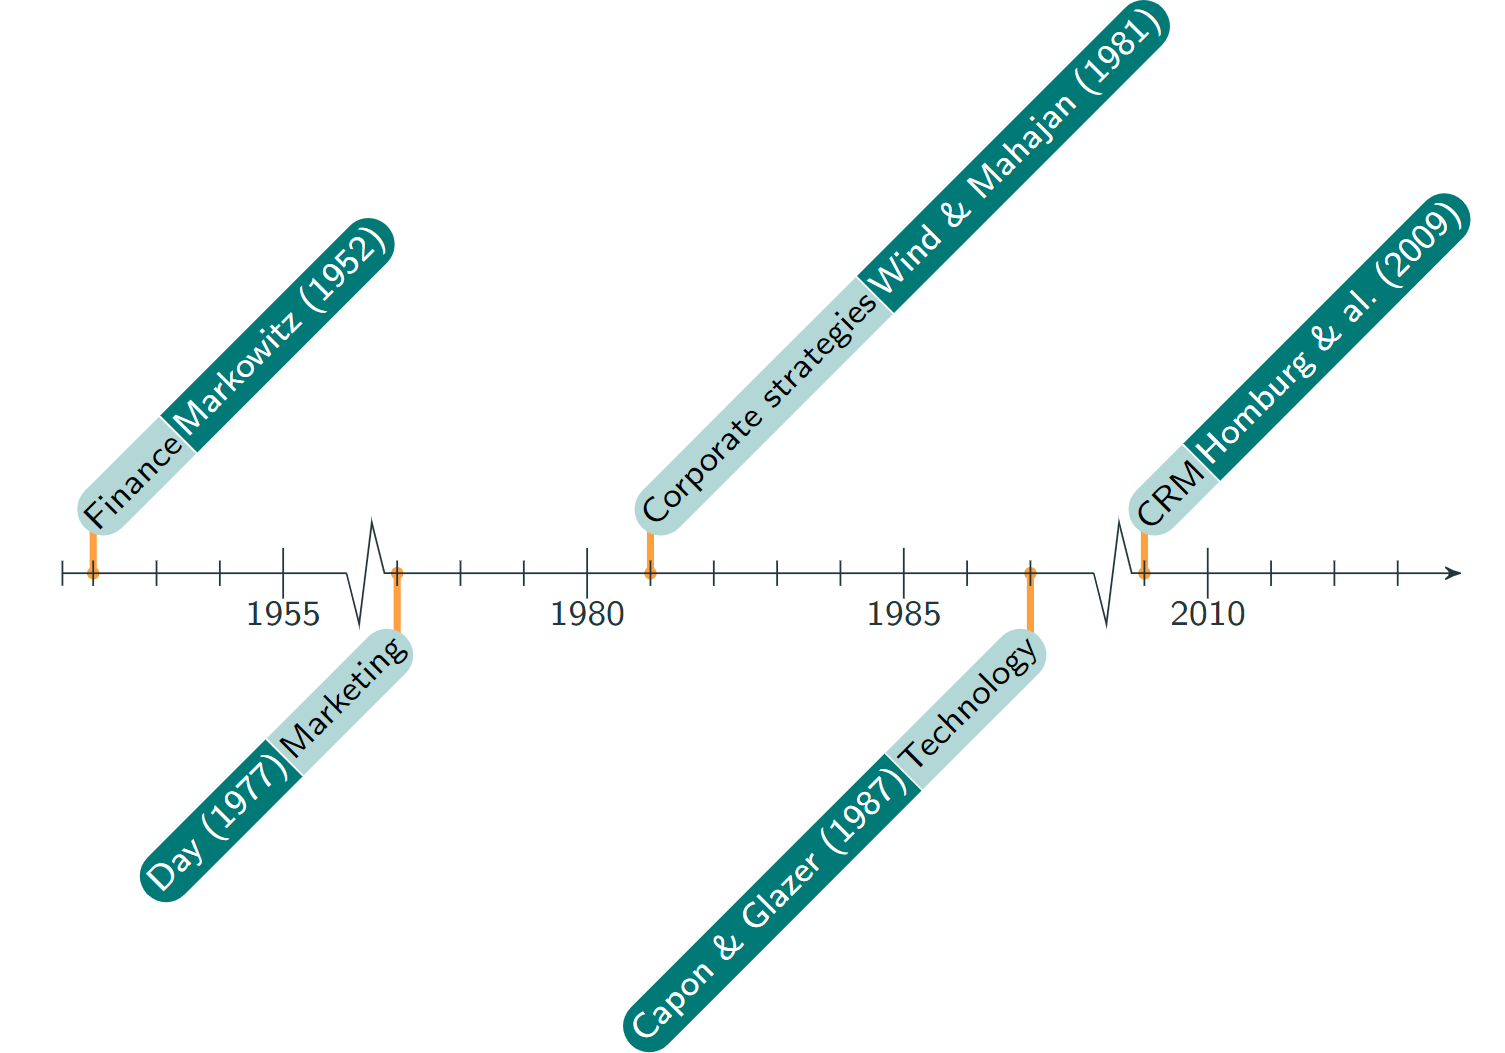
\includegraphics[width=400pt,height=300pt]{./imgs/portfolio_timeline} 

}

\caption{A timeline on the concept of portfolio}\label{fig:timeline}
\end{figure}

In their article \citet{CPM_CRM} examine how a company can define the
value of customers and segment these customers into portfolios. They explain how segmentation leads to better understanding of the relative importance of each customer to the company's total profit. The authors consider a \emph{portfolio} segmented into four groups of clients: \emph{platinum}, \emph{gold}, \emph{silver} and \emph{bronze} customers. The \emph{portfolio} segmentation is based both on the cost to serve a client as well as the latter's value to the firm, as depicted by figure \ref{fig:cpmmat}.

\begin{figure}

{\centering 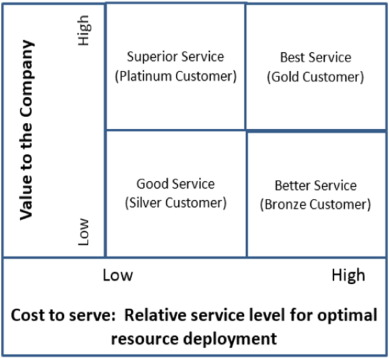
\includegraphics[width=250pt,height=250pt]{./imgs/cpm_matrix} 

}

\caption{CPM Matrix}\label{fig:cpmmat}
\end{figure}

According to this repartition into four main groups, Thakur and Workman highlight three strategies the firm can launch in order to efficiently manage its \emph{portfolio}. \textbf{Retention} aims to induce \emph{platinum} customers into repeating their purchases as they have a large contribution to the firm's revenue. \textbf{Customer relationship development} can be used to encourage customers to advance and upgrade to a higher segment. Such a strategy can be efficient for customers with high preference for a certain product or those with potential to shift to higher margin products. Conversely, \textbf{customer elimination or filtering} strategies are set up by the firm to encourage bottom customers who cost more than they are worth to leave the \textbf{portfolio}.

As said in the introduction, an interesting improvement of portfolio analysis may be to add a temporal dimension to the models. \citet{MANAGING_DYNAMICS_CUSTOMER_PORTFOLIO} show that the dynamic approach minimizes the current bias of underestimating low-value clients and overestimating high-value ones.

\hypertarget{attrition}{%
\section{On attrition}\label{attrition}}

\emph{Attrition} or churn has become a buzzword these last years. Churn analysis can be seen as an economic problem for three main reasons. Firstly, customers are in some way the firm's more precious asset. Secondly, the firm's resources in terms of customer relationship management are limited, so an efficient allocation needs to be deployed. Thirdly churn being a risk the firm has to cope with, it leads to asymmetric information from the firm's side. With the development of advanced Econometrics and Data Science, several methods can be implemented in order to estimate churn.

On the one hand, survival models are helpful in measuring customers' lifetime. In her thesis, \citet{SURV_METHODS_INSURANCE} applies duration analysis to model the behavior of customers from an insurance company with a threefold purpose:

\begin{itemize}
\tightlist
\item
  Identify factors influencing customer loyalty.
\item
  Estimate the remaining lifetime of a client who has purchased multiple policies and cancelled one of them.
\item
  Study the influence of covariates changing over time.
\end{itemize}

Her study is motivated by the importance of the insurer/policyholder relationship in a digitalized environment where the costs of searching for information are increasingly lower and the risk of \emph{attrition} consequently higher. The author develops a two-part methodology to address the study's problematic. She begins by solely selecting insureds with at least two policies. Then, she fits a logit model to predict whether a policyholder will cancel their policies at the same time (type 1) or sequentially (type 2). She finally applies duration models on type 2 clients to determine the remaining time until all their policies are cancelled.

On the other hand, machine learning classification algorithms can be used for churn detection as illustrated by the work of \citet{CHURN_INSURANCE}. Her objective is to develop a predictive model to detect customer churn in an insurance company while highlighting the key drivers of \emph{attrition}. The underlying goals of her research paper are both minimizing revenue loss caused by churn and boosting the firm's competitiveness. Using data on vehicle insurance policies, Bellani incorporates features on the policyholders, the vehicles, the insurance policies as well as marketing data to predict the churn indicator variable. After missing data imputation and dimensionality reduction, the author falls back on under-sampling to overcome the issue of unbalanced classes. There are indeed much more active than cancelled policies in the dataset. Her methodology works as follows:

\begin{itemize}
\tightlist
\item
  The set of active policies is divided into 7 groups equal in size to the number of cancelled policies.
\item
  For each group of active policies, classification models (logistic regression, random forest and neural network) are trained on a subset including all the cancelled policies as well as the concerned group of active ones.
\item
  For each model, the predictions are aggregated across the 7 subsets for the final prediction.
\item
  Model selection is made by the means of the Kappa performance metric.
\end{itemize}

Ultimately when a customer leaves the firm's portfolio, it may worth it to consider all possible outcomes for the reason he churned. For instance, a client might leave their telecom company because of a bad service quality, or because of too high a price. In this context, competing risk analysis can be introduced since its main interest is to determine the reason why the client churned. In their recent article, \citet{COMPETING_RISKS} try to predict both the likelihood of customer churn and the reasons for churn using customer service data from a Dutch TSP. They estimate duration and competing risk models. In the competing risk model, three possible output states are considered: Controllable risk, Uncontrollable risk and Unknown risk. Each type of risk is assumed independent from another which means a client cannot be at high risk for two risks simultaneously. Besides, the authors implement a Latent Dirichlet Allocation model (see \citet{LDA} for more details) to identify the main topics in a set of emails sent by customers to the service center. Six topics are discovered by the algorithm and each of them is then incorporated as explanatory variable into the models. These topic variables increase the performance of both competing risk models for Controllable and Unknown risks and standard duration models. According to Slof, Frasincar, and Matsiiako, \emph{``customers who churn due to the Controllable risk or due to the Unknown risk tend to call the customer service center with a specific problem, while customers who churn due to the Uncontrollable risk do not call the customer service center with a specific problem''}.

\hypertarget{value}{%
\section{On customer value}\label{value}}

In recent years, customer \emph{portfolio} management (CPM) has focused on optimizing clients' \emph{value} to the firm. The company's interest lies in knowing how much net benefit it can expect from a customer today. These expectations are then used to implement efficient marketing strategies to get the highest return on investment. To that end, two key metrics are estimated by firms: customer lifetime value (CLV) and customer equity (CE) (see part \ref{valuedef} in the introduction for definitions).

According to \citet{CLV_DEF}, CLV is atemporal variable defined as the revenue derived from a customer minus the cost to the firm for maintaining the relationship with this very customer. As shown by \citet{CLV_CONTEXT}, CLV modelling depends on the type of relationship a firm has with its clients. In a contractual relationship, customer defections are observed which means that longer lifetime means higher customer value. Conversely, when the relationship is non-contractual, uncertainty arises between the customer's purchase behavior and lifetime.

With the development of data collection tools, companies have lots of customer-level data (or customer transaction data) at their disposal to measure CLV \citep{CLV_NBD}. Consequently, different modelling approaches can be adopted in order to estimate customer \emph{value.}

Recency Frequency Monetary (RFM) models are considered the simplest strategy to measure CLV and customer loyalty \citep{CLV}. It aims at targeting specific marketing campaigns at specific groups of customers to improve response rates. RFM models consists in creating clusters of clients based on three variables:

\begin{itemize}
\tightlist
\item
  \emph{Recency} which is the time that has elapsed since a customer's last activity with the firm.
\item
  \emph{Frequency} that is the number of times a customer transacted with the brand in a particular period of time.
\item
  \emph{Monetary} that is to say the value of customer's prior purchases.
\end{itemize}

However, RFM models have a limited predictive power since they only predict clients' behavior for the next period.

In their article on CLV management, \citet{CLV_MEASUREMENT} draw the review of more advanced modelling techniques that can be implemented to estimate customers' \emph{value.} A popular method to estimate customer lifetime value is the negative binomial distribution (NBD) - Pareto \citep{CLV_NBD} which helps solving the lifetime uncertainty issue. The model takes past customer purchase behavior as input such as the number of purchases in a specific time window and the date of last transaction. Then the model outputs a repurchase probability as well as a transaction forecast for each individual. In Borle and Singh's research paper, a hierarchical bayesian model is implemented with a view to jointly predict customer's churn risk and spending pattern. Here, the main advantage of using a bayesian approach is to give priors on CLV's drivers. The study is based on data coming from a membership-based direct marketing company where firm/client relationships are non-contractual. In other words, the times of each customer joining the membership and terminating it are known once these events happen. Thus the implementation of a sophisticated estimation strategy is justified.

In our study, emphasize is placed on estimating the overall value of a customer portfolio. The methodology we will develop is based on a research paper written by our Econometrics teacher Alain Bousquet, whose goal is to provide tools for an efficient management of patent \emph{portfolios} \citep{BREVETS}. The main idea is to consider each patent as an asset with a related value which can generate income if this very patent is exploited. The author emphasizes the importance to focus on the \emph{portfolio}'s \textbf{variance} on top of its expected value. Specifically, he explains that the variability in the probability of success in the exploitation of patents leads to a decrease in the overall risk to which the \emph{portfolio} is exposed. This modelling approach can be transposed to customer \emph{portfolio} analysis with the customer's \emph{value} corresponding to the CLV and the probability of exploitation being the opposite of the risk of \emph{attrition}. In this context, CLV can be estimated either with techniques mentioned above or regression methods. The customer's risk of churn can be modelled with duration models or machine learning techniques as evoked in \ref{attrition}. With this econometric framework, it is expected that customer heterogeneity be a key factor in the total variance of the portfolio's \emph{value}.

\hypertarget{duration}{%
\chapter{Duration models}\label{duration}}

This chapter presents theoretical basis of the models that are used to model customer \emph{portfolios.} As a customer's lifetime in a \emph{portfolio} is usually represented by the time to churn, duration models are adapted to the data we have at our disposal. Thus, this part focuses on introducing standard survival techniques.

\hypertarget{definition}{%
\section{Definition}\label{definition}}

According to \citet{CAMERON_TRIVEDI}, duration models (also called survival models) aims at measuring the time spent in a certain state before transitioning to another state. In Econometrics,

\begin{itemize}
\tightlist
\item
  a \textbf{state} corresponds to the class in which an individual \(i\) is at time \(t\).
\item
  a \textbf{transition} is movement from one state to another.
\item
  a \textbf{duration} measures the time spent in a certain state and is also called a \textbf{spell} length.
\end{itemize}

Since measuring the time until the event is needed for multiple purposes, duration analysis is used in a variety of economic sectors as depicted by the following table.

\begin{longtable}[]{@{}cc@{}}
\toprule
Economic sector & Purpose \\
\midrule
\endhead
Macroeconomics & Length of unemployment spells \\
Insurance & Risk analysis to offer a segmented pricing \\
Engineering & Time until a device breaks down \\
Epidemiology & Survival time of a virus \\
\textbf{Churn analysis} & \textbf{Time until a customer leaves the portfolio} \\
\bottomrule
\end{longtable}

\hypertarget{censoring-and-truncation}{%
\section{Censoring and Truncation}\label{censoring-and-truncation}}

When dealing with survival data, some observations are usually \textbf{censored} meaning they are related to spells which are not completely observed. Duration data can also suffer from a selection bias which is called \textbf{truncation}.

\hypertarget{censoring-mechanisms}{%
\subsection{Censoring mechanisms}\label{censoring-mechanisms}}

\textbf{Left-censoring} occurs when the event of interest occurs before the beginning of the observation period. For example, an individual is included in a study of duration of unemployment at \(t_0\). At that time he has already been unemployed for a period but he cannot recall exactly the duration of this period. If we observe that he finds a job again at \(t_1\), we can only deduce that the duration of unemployment is bigger than \(t_1-t_0\), this individual is left-censored. Observation 2 on figure \ref{fig:censoring} is associated with a left-censored spell \citep{LIU_SCOR}.

A spell is considered \textbf{right-censored} when it is observed from time \(t_0\) until a censoring time \(t_c\) as illustrated by observation 1 on figure \ref{fig:censoring}. For instance, the lifetime related to a customer who has not churned at the end of the observation period is right-censored. Let us note \(X_i\) the duration of a complete spell and \(C_i\) the duration of a right-censored spell. We also note \(T_i\) the duration actually observed and \(\delta_i\) the censoring indicator such that \(\delta_i = 1\) if the spell is censored. Then \((t_1, \delta_1),\dots,(t_N, \delta_N)\) are the realizations of the following random variables:

\begin{equation}
  \begin{aligned}
  T_i & = \min(X_i, C_i) \\
  \delta_i & = \pmb{1}_{X_i > C_i}
  \end{aligned}
  \label{eq:censoring}
\end{equation}

\hypertarget{selection-bias}{%
\subsection{Selection bias}\label{selection-bias}}

Survival data suffers from a \textbf{selection bias} (or truncation) when only a sub-sample of the population of interest is studied. A customer entering the firm's \emph{portfolio} after the end of the study is said to be \textbf{right-truncated}, whereas a client who has left the \emph{portfolio} before the beginning of the study is considered \textbf{left-truncated}. Mathematically, a random variable \(X\) is truncated by a subset \(A \in \mathbb{R}^+\) if instead of \(\Omega(X)\), we solely observe \(\Omega(X)\bigcap A\). On figure \ref{fig:censoring}, the first and fifth observations suffers from a selection bias.

\begin{figure}

{\centering 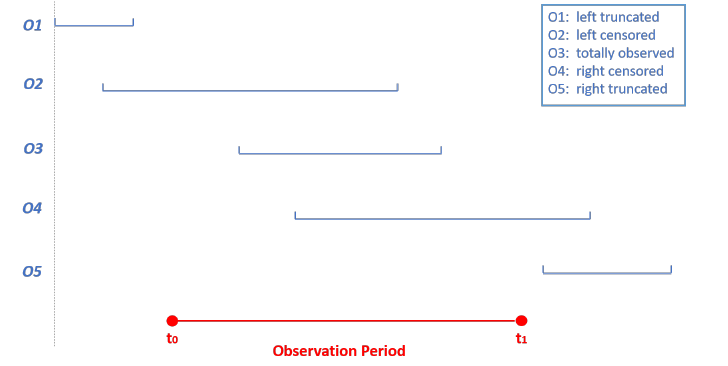
\includegraphics[width=500pt,height=250pt]{./imgs/censoring_and_truncation} 

}

\caption{Censored and truncated data}\label{fig:censoring}
\end{figure}

\hypertarget{probabilistic-concepts}{%
\section{Probabilistic concepts}\label{probabilistic-concepts}}

In survival analysis, the response variable denoted \(T\) is a time-to-event variable. Instead of estimating the expected failure time, survival models estimate the \textbf{survival} and \textbf{hazard rate} functions which depend on the realization of \(T\).

\hypertarget{survival-function}{%
\subsection{Survival function}\label{survival-function}}

The survival function \(S(t)\) represents the probability that the considered event occurs after time \(t\). For instance, \(S(t)\) can measure the probability that a given customer survives in the \emph{portfolio} at least until time \(t\). Mathematically, the survival function is defined as:
\begin{equation}
  S(t) = P(T > t) = 1 - F(t)
  \label{eq:survfun}
\end{equation}

where \(F(t)\) is the cumulative distribution function.

\begin{figure}

{\centering 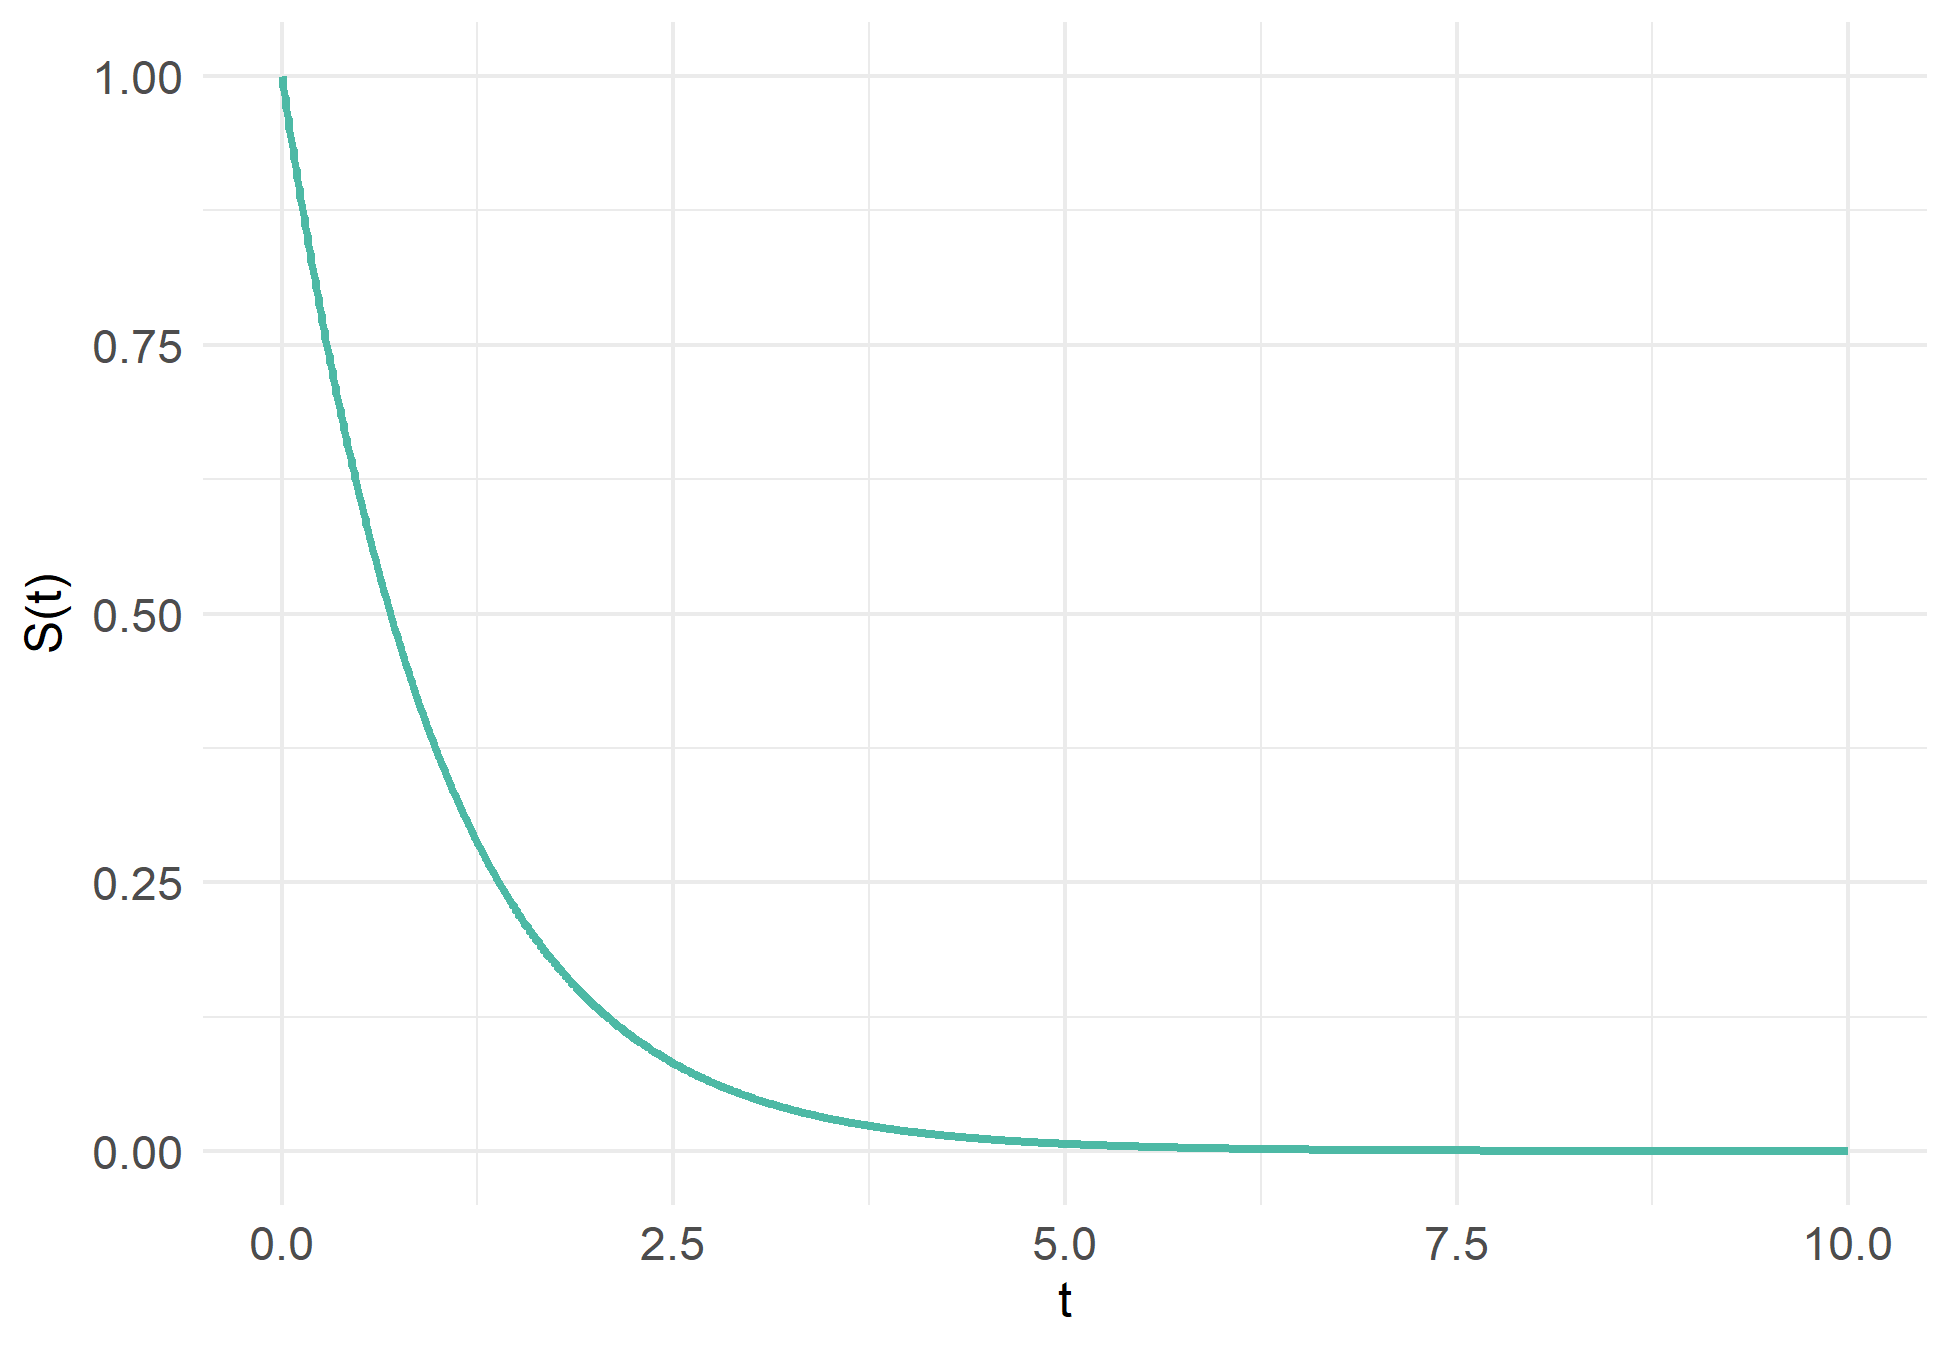
\includegraphics[width=400pt,height=300pt]{./imgs/surv_fun_plot} 

}

\caption{Survival function $S_T(t)$ with $T \sim \mathcal{E} (1)$}\label{fig:survfunplot}
\end{figure}

\hypertarget{hazard-and-cumulative-hazard-functions}{%
\subsection{Hazard and Cumulative Hazard functions}\label{hazard-and-cumulative-hazard-functions}}

Another key concept in duration analysis is the hazard function \(\lambda(t)\) which approximates the probability that the event occurs at time \(t\). For instance, \(\lambda(t)\) can measure the probability that a given individual leaves the firm \emph{portfolio} at time \(t\). Formally, it is expressed as follows:
\begin{equation}
  \lambda(t) = \lim_{\Delta t \to 0} \frac{P\big[t \leq T < t + \Delta t | T \geq t \big]}{\Delta t}
  \label{eq:hazfun}
\end{equation}

Using the Bayes formula, equation \eqref{eq:hazfun} can also be written as (see proof \eqref{eq:hazfunproof} in the appendix):
\begin{equation}
  \lambda(t) = \frac{-\text{d} \ln \big(S(t)\big)}{\text{d} t}
  \label{eq:hazfunbis}
\end{equation}

Finally, integrating the instantaneous hazard function gives the cumulative hazard function which can be more precisely estimated than the hazard function \citep{CAMERON_TRIVEDI} and is defined as:

\begin{equation}
  \Lambda (t) = \int_{0}^{t} \lambda(s) \text{d}s = \ln \big(S(t)\big)
  \label{eq:cumhazfun}
\end{equation}

\begin{figure}

{\centering 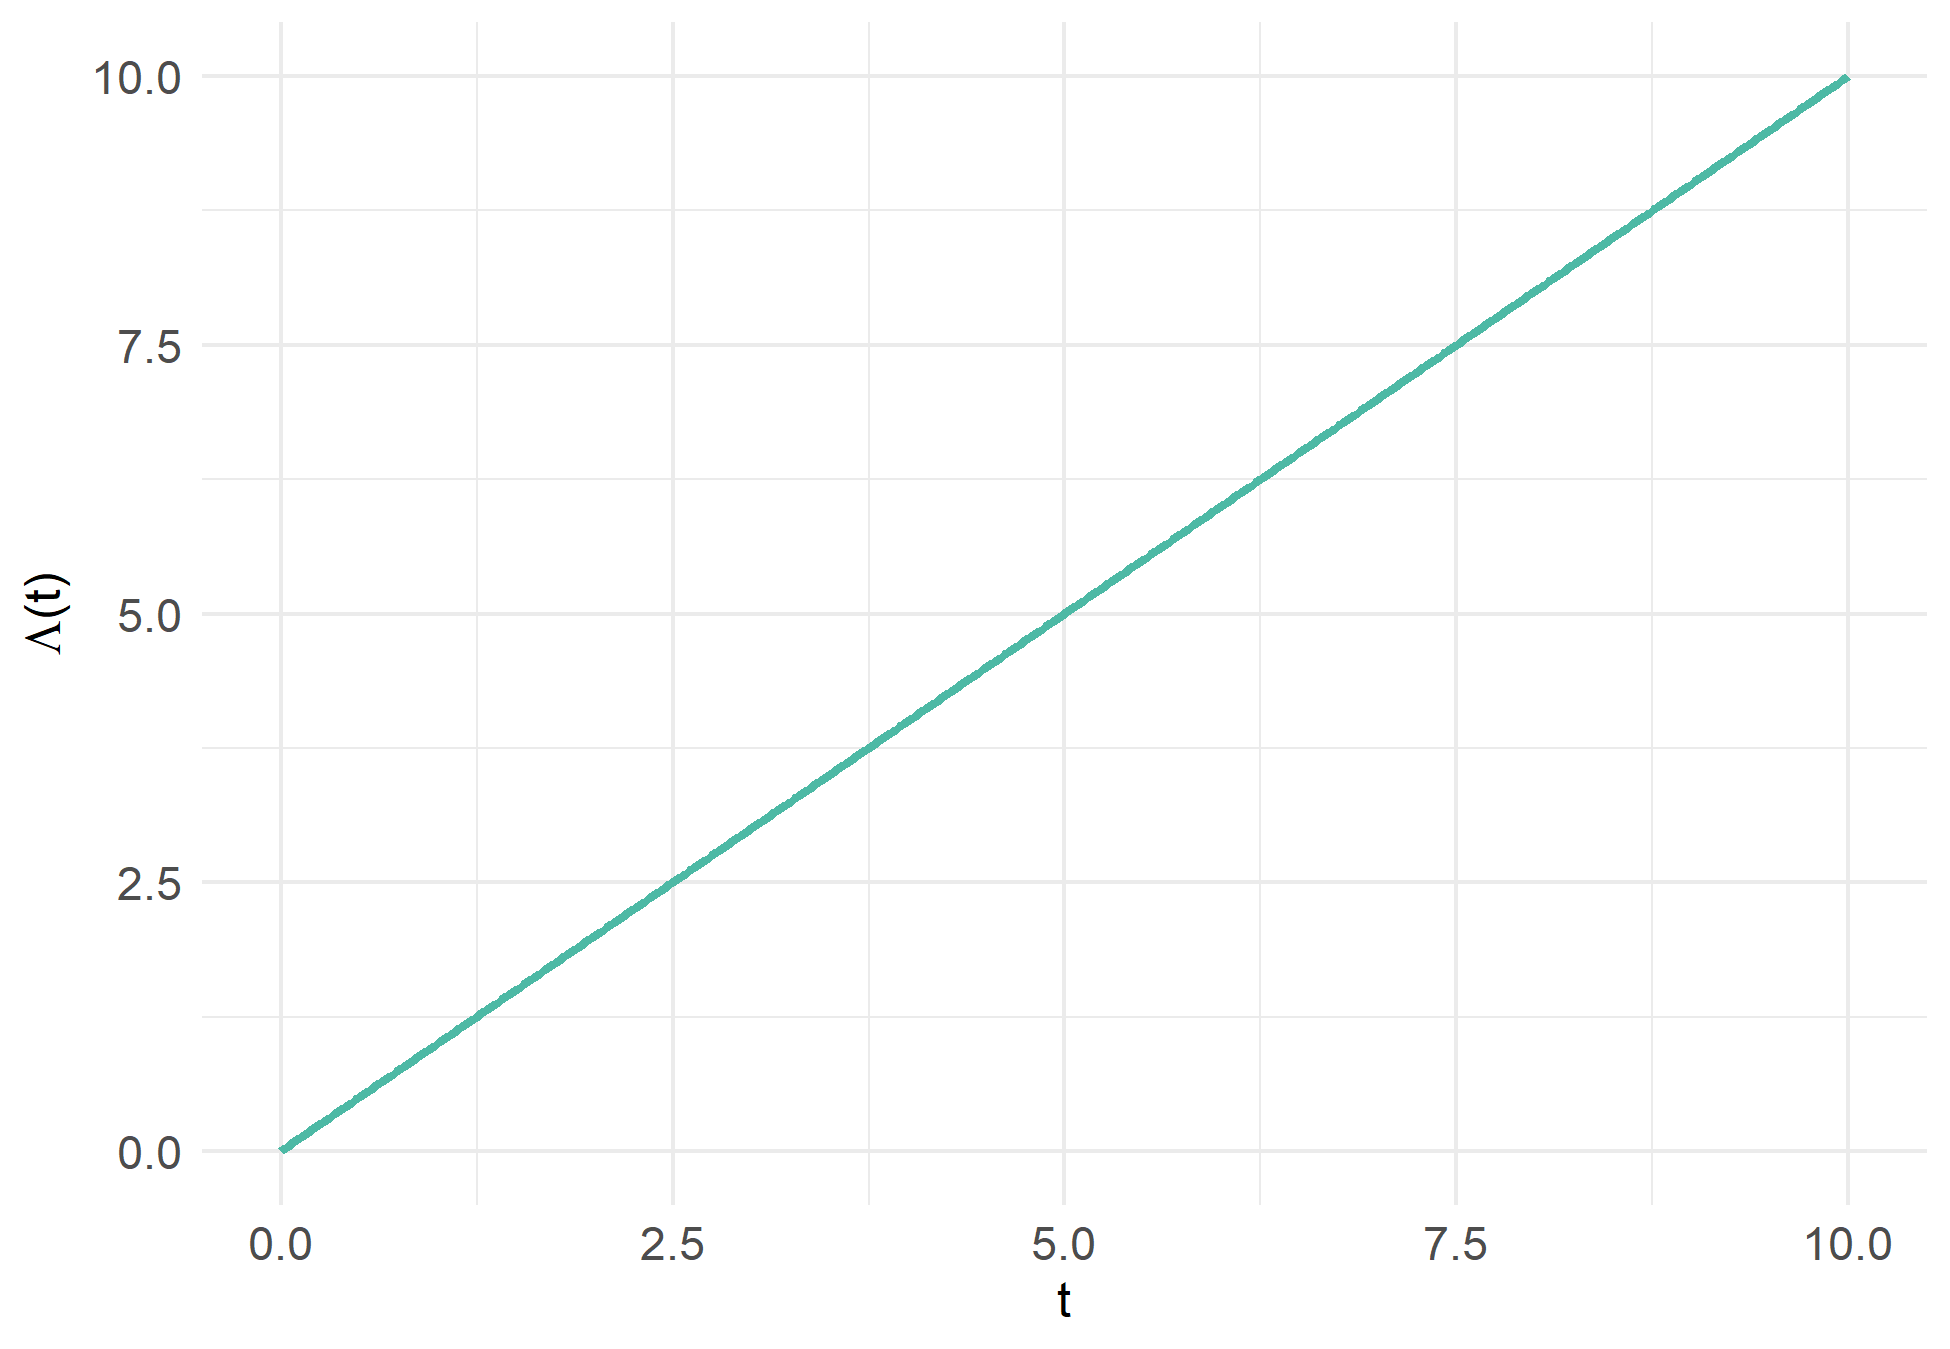
\includegraphics[width=400pt,height=300pt]{./imgs/cum_haz_plot} 

}

\caption{Cumulative Hazard function $\Lambda_T(t)$ with $T \sim \mathcal{E} (1)$}\label{fig:cumhazplot}
\end{figure}

Thus, \textbf{the hazard, survival and cumulative hazard functions} are three mathematical functions which describe the same distribution.

\hypertarget{nonparam}{%
\section{Nonparametric models}\label{nonparam}}

When dealing with duration data, these methods are helpful to have a general overview of the raw (unconditional) hazard. Nonparametric models are rather used for data description rather than prediction. No explanatory variable is included in these models except for treatment variables such as the type of contract a customer has subscribed.

\hypertarget{notations}{%
\subsection{Notations}\label{notations}}

Let us consider a sample with \(N\) observations with \(k\) discrete failure times (e.g.~a failure can be a churn event), such that \(\forall j \in [\![1; k]\!]\) :

\begin{itemize}
\tightlist
\item
  \(t_j\) the \(j^{\text{th}}\) discrete failure time,
\item
  \(d_j\) the number of spells terminating at \(t_j\),
\item
  \(m_j\) the number of right-censored spells in the interval \([t_j, t_{j+1}]\),
\item
  \(r_j\) the number of exposed durations right before time \(t_j\) i.e.~at time \(t_j^{-}\), such that:
  \begin{equation}
  r_j = (d_j + m_j) + \dots + (d_k + m_k) = \sum_{l|l \geq j} (d_l + m_l)
  \label{eq:exposed}
  \end{equation}
\end{itemize}

\hypertarget{hazard-function-estimator}{%
\subsection{Hazard function estimator}\label{hazard-function-estimator}}

As the instantaneous hazard at time \(t_j\) is defined as \(\lambda_j = P[T=t_j|T\geq t_j]\), a trivial estimator of \(\lambda_j\) is obtained by dividing the number of durations for which the event is realized at \(t_j\) by the total number of exposed durations at time \(t_j^{-}\). Formally, it is expressed as:

\begin{equation}
  \hat{\lambda}_j = \frac{d_j}{r_j}
  \label{eq:hazest}
\end{equation}

\hypertarget{kaplan-meier-estimator}{%
\subsection{Kaplan-Meier estimator}\label{kaplan-meier-estimator}}

Once the hazard function estimator computed, the discrete-time survivor function can be estimated using the Kaplan-Meier product-limit estimator. To estimate the survival at time \(t\), this estimator computes the joint probability that a spell stays in the same state until \(t\) (e.g.~remaining loyal to a firm until a certain time). This method is based on conditional probabilities and the survival function estimate is defined as:

\begin{equation}
  \hat{S}(t) = \Pi_{j|t_j \leq t} \big(1-\hat{\lambda}_j\big) = \Pi_{j|t_j \leq t}\frac{r_j - d_j}{r_j}
  \label{eq:kaplanmeier}
\end{equation}

When plotting the survival curve after having performed the Kaplan-Meier estimation, confidence bands are also added to the plot in order to reflect sampling variability \citep{CAMERON_TRIVEDI}. The confidence interval of the survival function \(S(t)\) is derived from the estimate of the variance of \(S(t)\) which is obtained by the Grenwood estimate as in equation \eqref{eq:greenwood}.

\begin{equation}
  \hat{\mathrm{V}}[\hat{S}(t)] = \hat{S}(t)^2 \sum_{j|t_j \leq t} \frac{d_j}{r_j(r_j-d_j)}
  \label{eq:greenwood}
\end{equation}

\hypertarget{nelson-aalen-estimator}{%
\subsection{Nelson-Aalen estimator}\label{nelson-aalen-estimator}}

The cumulative hazard function estimate is given by the Nelson-Aalen estimator which consists in summing up the hazard estimates for each failure time.

\begin{equation}
  \hat{\Lambda}(t) = \sum_{j | t_j \leq t} \hat{\lambda}_{j} = \sum_{j | t_j \leq t} \frac{d_j}{r_j}
  \label{eq:nelsonaalen}
\end{equation}

Exponentiating \(\hat{\Lambda}(t)\), one can obtain a second estimate of the survival function (see proof \eqref{eq:linksurvcumhaz} in the appendix):

\begin{equation}
    \tilde{S}(t) = \exp \big( -\hat{\Lambda}(t) \big)
    \label{eq:survest}
\end{equation}

\hypertarget{parametric-models}{%
\section{Parametric models}\label{parametric-models}}

The nonparametric estimation is undoubtedly useful when it comes to have a general overview on the survival data. However, one may want to model the hazard and survivor functions with a functional form in which unknown parameters need to be optimized.

When implementing parametric models, \(\lambda\), \(S\) and \(\Lambda\) are expressed based on the chosen parametric form. The instantaneous hazard function can either be constant or monotone.

In our study we assume that the explanatory variables are time-constant as we do not have dynamic data at our disposal. Thus, solely time-invariant duration models are presented.

Parametric estimation has a twofold purpose that is to implement a robust model to estimate the risk that a specific event occurs while identifying the variables (or covariates) which best explain this risk.

\hypertarget{constant-hazard-exponential-model}{%
\subsection{Constant hazard (exponential model)}\label{constant-hazard-exponential-model}}

The exponential distribution models the time between events in a Poisson process and has the key property of being \emph{memoryless}. Let us note \(T\) a time-to-event variable such that \(T \sim \mathcal{E}(\theta)\) where \(\theta\) is the rate parameter. In this context, \emph{memorylessness} can be defined as follows:

\begin{equation}
  \mathbb{P}(T>t+s | T > t) = \mathbb{P}(T>s)
  \label{eq:memorylessness}
\end{equation}

\(\forall t \geq 0\ ,\ \theta > 0\) the density, hazard and survival functions can be expressed as:

\begin{equation}
  \begin{aligned}
    f_{\theta}(t) & = \theta e^{-\theta t} \\\\
    \lambda_{\theta}(t) & = \theta \\\\
    S_{\theta}(t) & = e^{-\theta t} \\\\
  \end{aligned}
  \label{eq:exponential}
\end{equation}

Thus, the exponential distribution is characterized by a \textbf{constant} hazard function which is a consequence of the \emph{memorylessness} property.

\hypertarget{monotone-hazard}{%
\subsection{Monotone hazard}\label{monotone-hazard}}

\hypertarget{weibull-model}{%
\subsubsection*{Weibull model}\label{weibull-model}}
\addcontentsline{toc}{subsubsection}{Weibull model}

The Weibull distribution is a less restrictive generalization of the exponential distribution defined by a shape parameter \(\nu\) and a scale parameter \(\theta\).

\(\forall t \geq 0\) and \(\nu,\ \theta > 0\) the density, hazard and survival functions can be expressed as:

\begin{equation}
  \begin{aligned}
      \lambda_{\nu,\theta}(t) & = \nu \bigg(\frac{1}{\theta}\bigg)^{\nu} t^{\nu - 1} \\\\
      S_{\nu, \theta}(t) & = \exp \Bigg( -\bigg(\frac{1}{\theta}\bigg)^{\nu} t\Bigg) 
  \end{aligned}
  \label{eq:weibull}
\end{equation}

The instantaneous hazard function \(\lambda_{\nu,\theta}\) is monotonic \textbf{decreasing} if \(\nu \in [0, 1]\). For instance, the \emph{attrition} risk may decrease as the customer's duration in the \emph{portfolio} increases. In this context, the client gets more and more loyal to the firm. If \(\nu=1\), the hazard rate is constant and \(T \sim \mathcal{E}(\theta)\). Converlsely, the hazard function is monotonic \textbf{increasing} if \(\nu > 1\). This can be the case when customers tend to continuously search for information on the firm's competitors, thus becoming more likely to churn as time goes by.

Figure \ref{fig:weibullplots} illustrates the hazard and survivor functions associated to a Weibull-distributed variable \(T\). The two curves' shape depend both on the shape (\(\nu\)) and scale (\(\theta\)) parameters. Some remarks can be made looking at the two plots. When \(\nu < 1\) the hazard function is decreasing meaning that the risk of the event occurring decreases as time goes by. When \(\nu > 1\) the hazard function is convex which indicates that a marginal increase in time leads to an increase (decrease) of over one unit in the the hazard (survivor) function. The higher the shape parameter, the more increasing the hazard function. When \(\nu = \theta = 1\), it can be noted that the Weibull distribution corresponds to the exponential distribution (see figures \ref{fig:survfunplot} and \ref{fig:cumhazplot}).

\begin{figure}

{\centering 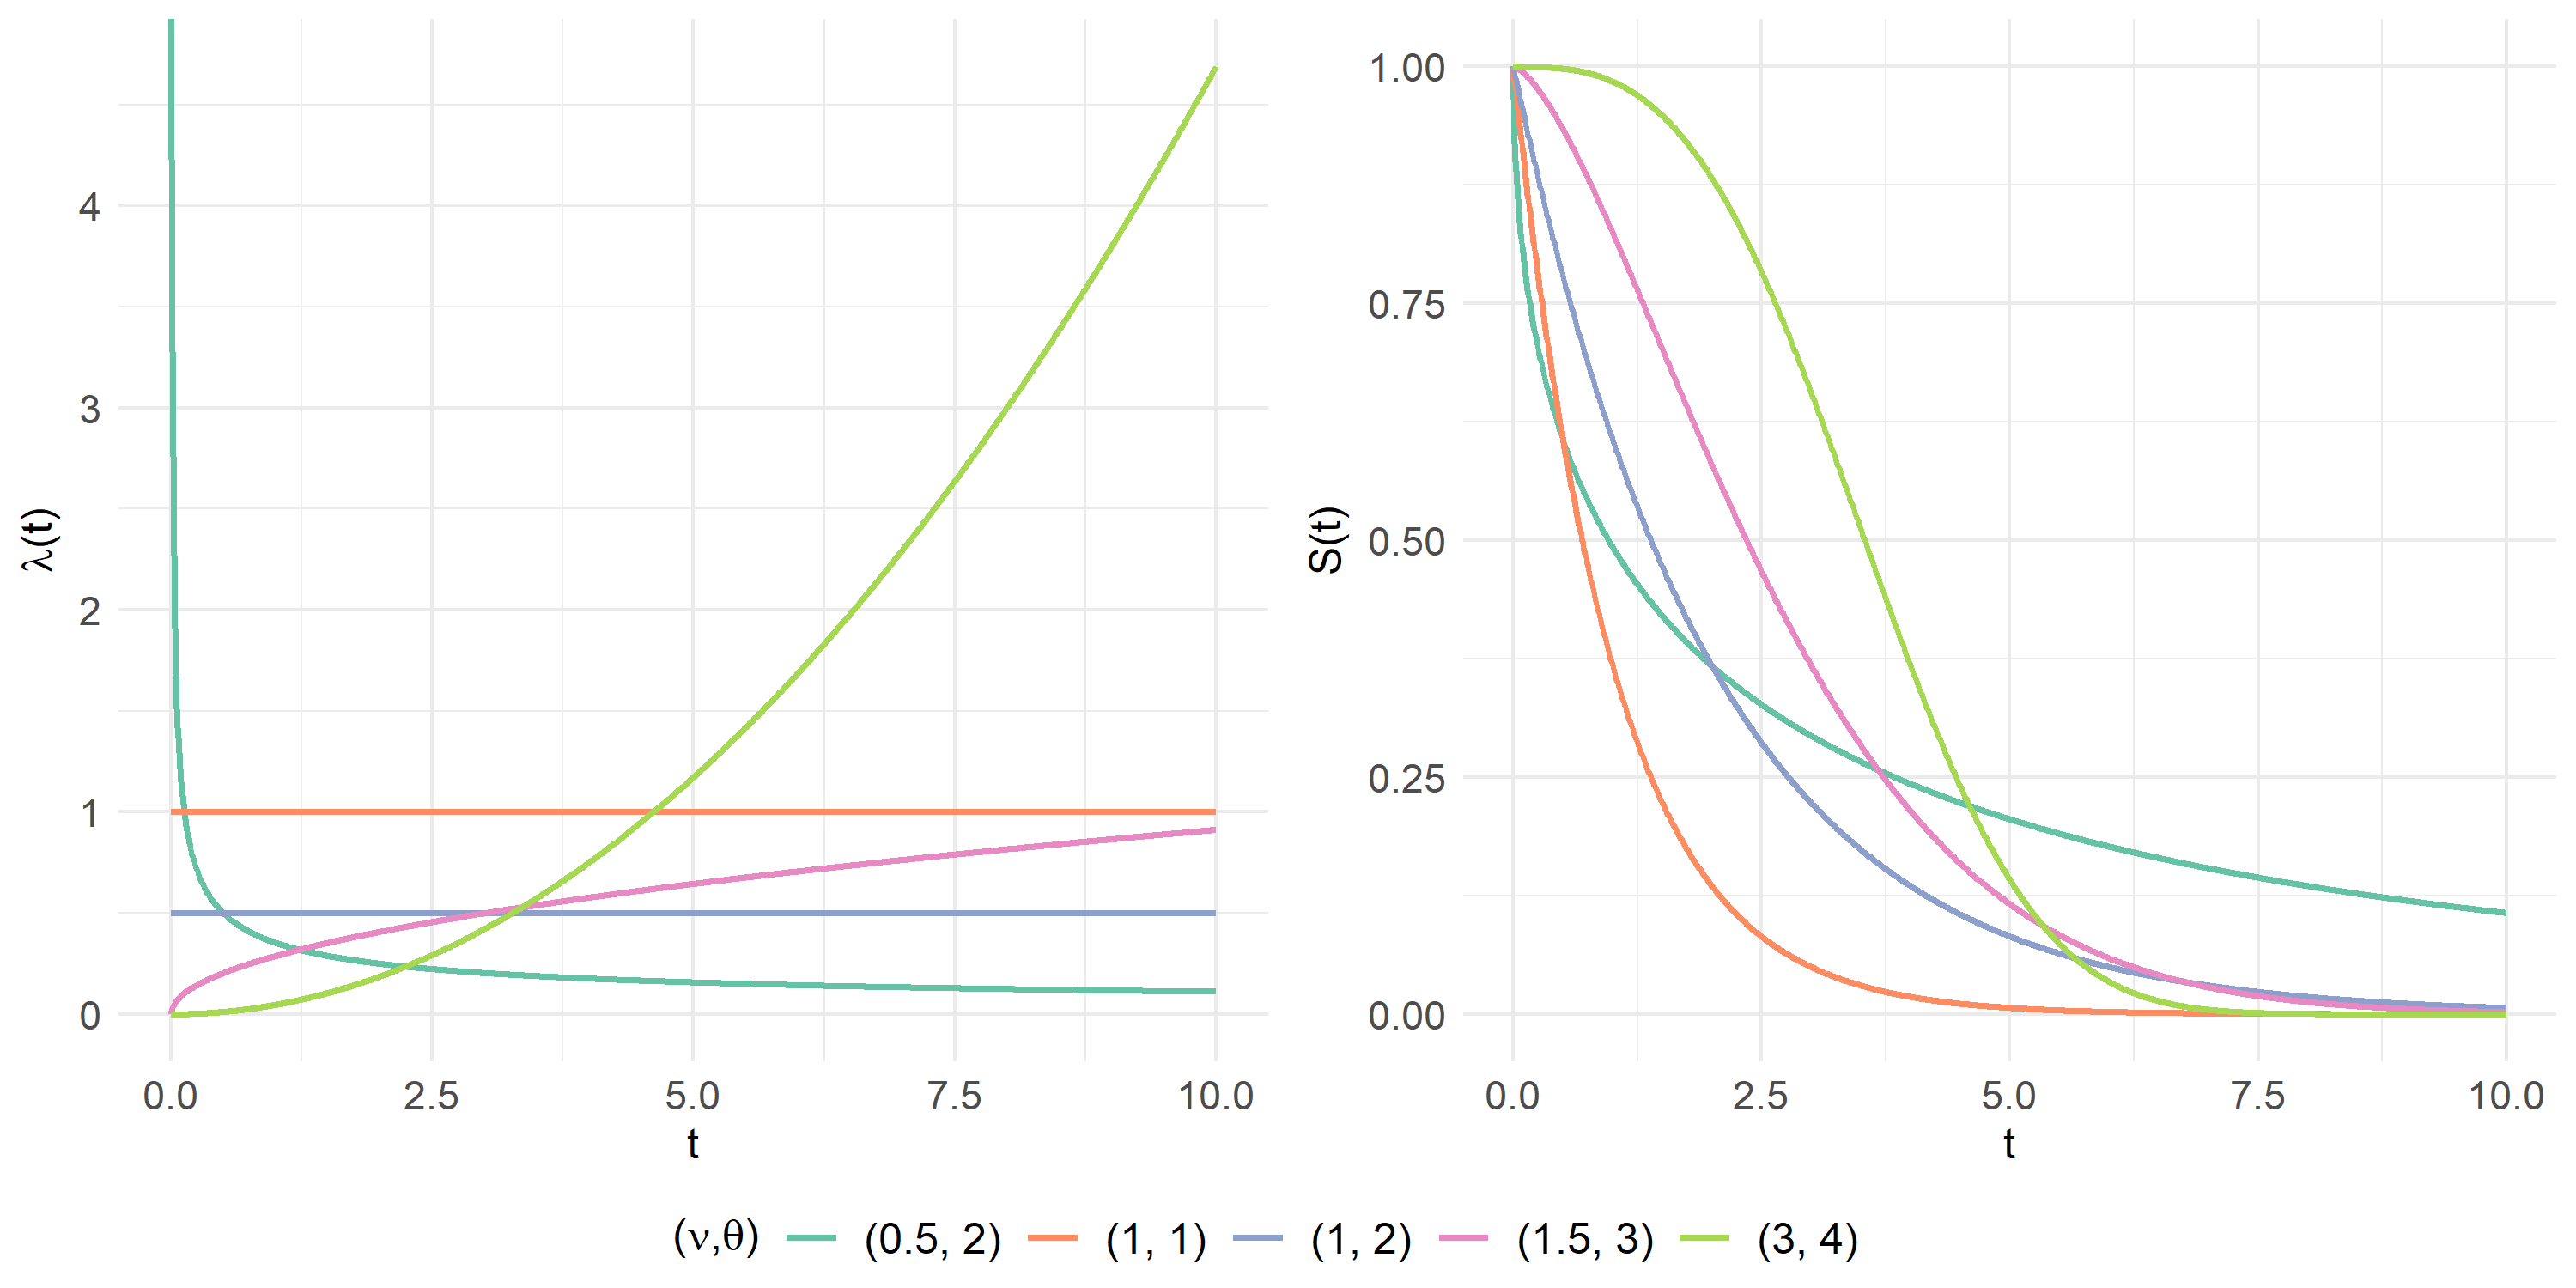
\includegraphics[width=700pt,height=350pt]{./imgs/weibull_plots} 

}

\caption{Hazard and Survival functions with $T \sim \mathcal{W} (\nu, \theta)$}\label{fig:weibullplots}
\end{figure}

\hypertarget{other-models}{%
\subsubsection*{Other models}\label{other-models}}
\addcontentsline{toc}{subsubsection}{Other models}

Different probabilistic distributions can be chosen to model the hazard and survival functions related to a time-to-event variable. The Gompertz model is usually used for mortality data in biostatistics. The gamma model depends both on the gamma and inverse-gamma distributions and is also based on shape and scale parameters.

\hypertarget{concave-and-convex-hazard}{%
\subsection{Concave and convex hazard}\label{concave-and-convex-hazard}}

When the hazard function does not evolve in a monotonic fashion, the distributions introduced above are limited. The generalized Weibull model appears to be a good choice to estimate phenomena with concave or convex hazards. It is based on three parameters: \(\nu\) (shape), \(\theta\) (scale) and \(\gamma\). When \(\gamma = 1\), the generalized Weibull becomes the Weibull distribution \(\mathcal{W}(\nu, \theta)\).

\hypertarget{semi-parametric-estimation}{%
\section{Semi-parametric estimation}\label{semi-parametric-estimation}}

\hypertarget{proportional-hazards-models}{%
\subsection{Proportional Hazards models}\label{proportional-hazards-models}}

Parametric models assume that the baseline (or raw) hazard follows a specific distribution. This assumption can be sometimes too restrictive and semi-parametric models can be more adapted to describe the duration data.

In \emph{proportional hazards} (PH) models, the instantaneous risk function is \textbf{proportional} to the baseline hazard \(\lambda_0 (t,\alpha)\) modulo a \textbf{scaling factor} depending on the covariates \(\phi(\pmb{\mathrm{x}}, \beta)\). These models allow to generalize the basic survival models to a survival regression model which permits to take individuals' heterogeneity into consideration \citep{RMS}. The general mathematical formulation is expressed as follows:

\begin{equation}
    \lambda(t|\pmb{\mathrm{x}}) = \lambda_0 (t,\alpha)  \phi(\pmb{\mathrm{x}}, \beta) 
    \label{eq:ph}
\end{equation}

Note that when the function form of \(\lambda_0 (t,\alpha)\) is known, we are in the case of parametric estimation. For instance, the exponential, Weibull and Gompertz models are PH models since their respective hazards are function of some covariates.

\hypertarget{what-does-proportional-hazards-mean}{%
\subsubsection*{\texorpdfstring{What does \emph{proportional hazards} mean?}{What does proportional hazards mean?}}\label{what-does-proportional-hazards-mean}}
\addcontentsline{toc}{subsubsection}{What does \emph{proportional hazards} mean?}

PH models are said to be proportional as the relative hazard ratio between two individuals \(i\) and \(k\) does not vary over time, such that:

\begin{equation}
  \frac{\lambda(t|\mathrm{x_i})}{\lambda(t|\mathrm{x_k})} = \frac{\phi(\mathrm{x_i}, \beta) }{\phi(\mathrm{x_k}, \beta)}
  \label{eq:prophazratio}
\end{equation}

The formulation stated in equation \eqref{eq:prophazratio} needs to be verified when one wants to fit a PH model to real-life data.

\hypertarget{marginal-effects}{%
\subsubsection*{Marginal effects}\label{marginal-effects}}
\addcontentsline{toc}{subsubsection}{Marginal effects}

In \emph{proportional hazards} models, the marginal effect of covariate \(x_p\) on the hazard function can be easily derived since this computation only requires knowledge on \(\beta\). As shown in \citet{CAMERON_TRIVEDI}, a one-unit increase in the \(p^{\text{th}}\) covariate leads to the following variation in the hazard function \emph{ceteris paribus}:

\begin{equation}
    \frac{\partial \lambda(t|\pmb{\mathrm{x}}, \beta)}{\partial x_p} = \lambda(t|\pmb{\mathrm{x}}, \beta) \frac{\partial \phi(\pmb{\mathrm{x}}, \beta) / \partial x_p}{\phi(\pmb{\mathrm{x}}, \beta) }
    \label{eq:meph}
\end{equation}

\hypertarget{partial-likelihood-estimation}{%
\subsubsection*{Partial likelihood estimation}\label{partial-likelihood-estimation}}
\addcontentsline{toc}{subsubsection}{Partial likelihood estimation}

The vector of parameters \(\beta\) related to the regression part of the PH model is estimated by partial likelihood maximization. The method's principle consists in only estimating the regression's parameters \(\beta\) by considering the baseline hazard \(\lambda_0\) as noise. If desired an estimate of the baseline hazard can be recovered after estimation of \(\beta\) using, for instance, the Nelson-Aalen estimator (see part \ref{nonparam}). Cox's intuition is that no information can be retrieved from the intervals during which no event has occurred and that it is conceivable that \(\lambda_0\) is null in these intervals. Thus, solely the set of moments when an event occurs are considered in the estimation method.

In order to derive the partial likelihood function, let us note \(t_j\) the \(j^{\text{th}}\) discrete failure time in an \(N\)-sample with \(j \in [\![1; k]\!]\), such that:

\begin{itemize}
\tightlist
\item
  \(t_1 < t_2 < \dots < t_k\),
\item
  \(D(t_j) = \{l: t_l = t_j\}\) is the set of spells completed at \(t_j\) with \(\#D(t_j) = d_j\),
\item
  \(R(t_j) = \{l: t_l \geq t_i\}\) is the set of spells at risk at \(t_j\).
\end{itemize}

The contribution of a spell in \(D(t_j)\) to the likelihood function equals the conditional probability that the spell ends at \(t_j\) given it is exposed at that specific time and can be written as (see \citet{CAMERON_TRIVEDI} and proof \eqref{eq:contribpartiallikproof} for more details):

\begin{equation}
  \mathbb{P}\big[T_j = t_j | R(t_j) \big] = \frac{\phi(\mathrm{x_j}, \beta)}{\sum_{l \in R(t_j)} \phi(\mathrm{x_l}, \beta)}
  \label{eq:contribpartiallik}
\end{equation}

Given \(k\) discrete failure times are considered and that for each of those there is a set \(D(t_j)\) of completed spells, Cox defines the partial likelihood function as the joint product of the probability expressed in \eqref{eq:contribpartiallik}, such that:

\begin{equation}
  \mathcal{L}_p = \Pi_{j=1}^{k} \ \frac{\Pi_{m \in D(tj)} \ \phi(\mathrm{x_j}, \beta)}{\Big[\sum_{l \in R(t_j)} \phi(\mathrm{x_l}, \beta)\Big]^{d_j}}
  \label{eq:partlik}
\end{equation}

The latter formulation of the partial likelihood function is explained in more details in equations \eqref{eq:partlikproof} and \eqref{eq:partlikproofbis} in the appendix.

\hypertarget{cox-ph-model}{%
\subsection{Cox PH model}\label{cox-ph-model}}

The Cox \emph{proportional hazards} model is the most popular for the analysis of duration data. This model is said to be semi-parametric as it makes no assumption regarding the nature of the baseline hazard function \(\lambda_0(t)\). The parametric part only relies in the modelling of the effect of some covariates on the hazard function \(\lambda(t)\). The relationship between the vector of covariates and the log hazard is linear and the parameters can be estimated by maximizing the partial likelihood function. The Cox PH model solely assumes that predictors act multiplicatively on the hazard function. The model is formulated as in equation \eqref{eq:ph} with the exponential function as link between the hazard and the covariates i.e.~\(\lambda(t|\pmb{\mathrm{x}}) = \lambda_0 (t,\alpha) \text{e}^{\pmb{\mathrm{x'}} \beta}\).

\hypertarget{ml}{%
\chapter{Machine Learning}\label{ml}}

\emph{A computer program is said to learn from experience \(E\) with respect to some class of tasks \(T\) and performance measure \(P\) if its performance at tasks in \(T\), as measured by \(P\), improves with experience \(E\).}

\emph{-- Tom M. Mitchell --}

This chapter introduces machine learning algorithms used to model customer \emph{portfolio}. We firstly explain the techniques which aim to enrich the standard survival tools defined in the previous chapter. A second part depicts some regression models that are robust to predict customer lifetime value. Finally, the prediction performance associated to predictive methods are described.

\hypertarget{machine-learning-for-survival-data}{%
\section{Machine Learning for Survival Data}\label{machine-learning-for-survival-data}}

In chapter \ref{duration}, some important models for duration data have been introduced. Here, emphasize is placed on machine learning algorithms that can also be implemented to predict a time-to-event variable such as the time to churn.

\hypertarget{survival-trees}{%
\subsection{Survival Trees}\label{survival-trees}}

Traditional decision trees, also called CART (Classification And Regression Trees), segment the feature space into multiple rectangles and then fit a simple model to each of these subsets as shown by figure \ref{fig:tree} \citep{ML_TREE}. The algorithm is a recursive partitioning which requires a criterion for choosing the \emph{best} split, another criterion for deciding when to stop the splits and a rule for predicting the class of an observation.

\begin{figure}

{\centering 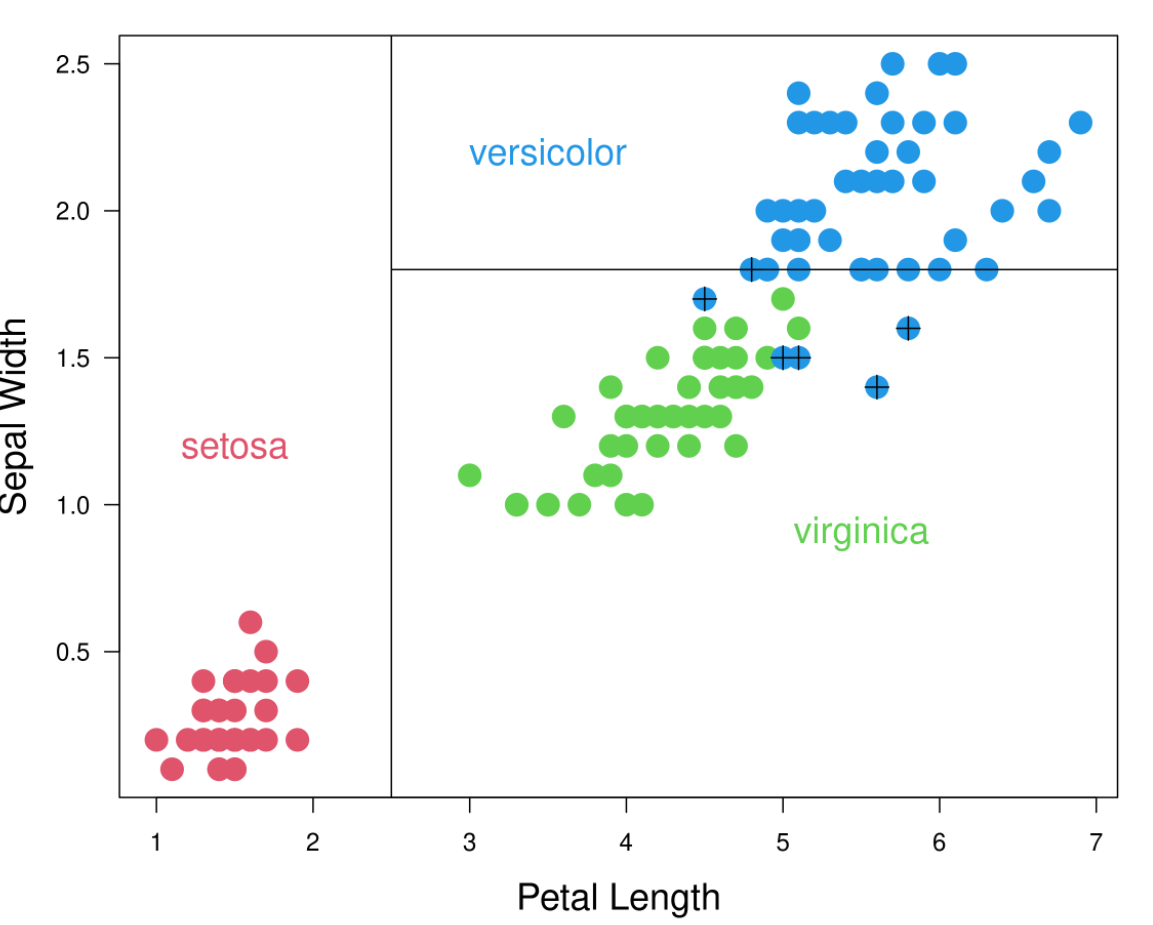
\includegraphics[width=0.45\linewidth,height=260pt]{./imgs/tree1} 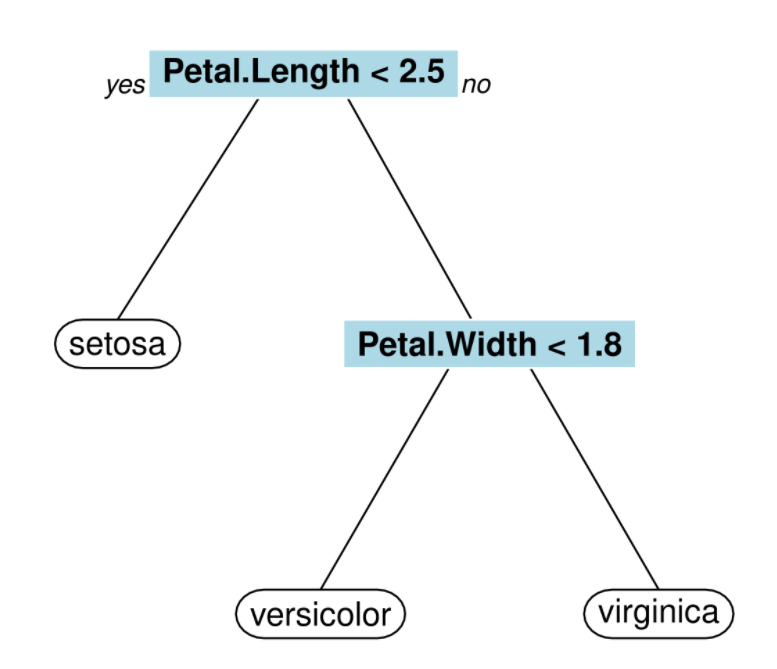
\includegraphics[width=0.45\linewidth,height=260pt]{./imgs/tree2} 

}

\caption{Clasification decision tree}\label{fig:tree}
\end{figure}

Survival tree \citep{SURV_TREE} is the adapted version of CART for duration data. The objective is to use tree based binary splitting algorithm in order to predict hazard rates. To that end, survival time and censoring status are introduced as response variables. The splitting criteria used for survival trees have the same purpose than the criteria used for CART that is to say maximizing between-node heterogeneity or minimizing within-node homogeneity. Nonetheless, node purity is different in the case of survival trees as a node is considered pure if all spells in that node have similar survival duration. The most common criterion is to use the \textbf{logrank test} statistic to compare the two groups formed by the children nodes. For each node, every possible split on each feature is being examined. The best split is the one maximizing the survival difference
between two children nodes. The test statistic is \(\chi^2\) distributed which means the higher its value, the higher between-node variability so the better the split.

\hypertarget{random-survival-forests-rsf}{%
\subsection{Random Survival Forests (RSF)}\label{random-survival-forests-rsf}}

This algorithm is proposed by \citet{RSF} and is an ensemble of decision trees for the analysis of right-censored survival data. As random forests used for regression and classification, RSF are based on \textbf{bagging} which implies that \(B\) bootstrap samples are drawn from the original data with 63\(\%\) of them are in the bag data and the remaining part is in the out-of-bag (OOB) data. For each bootstrap sample, a survival tree is grown based on \(p\) randomly selected features. Then, the parent node is split using the feature among the selected ones that maximizes survival difference between children nodes. Each tree is grown to full size and each terminal node needs to have no less than \(d_0\) unique events. The cumulative hazard function (CHF) is computed for each tree using the Nelson-Aalen estimator such as:

\begin{equation}
  \widehat{H_l}(t) = \sum_{t_{j, l} < t} \frac{d_{j,l}}{r_{j,l}}
  \label{eq:chf}
\end{equation}

where \(t_{j,l}\) is the \(j^{\text{th}}\) distinct event time in leaf \(l\), \(d_{j,l}\) the number of events completed at \(t_{j,l}\) and \(r_{j,l}\) the number of spells at risk at \(t_{j,l}\).

All the CHFs are then averaged to obtain the bootstrap ensemble CHF and prediction error is finally computed on the OOB ensemble CHF.

\hypertarget{cox-boosting}{%
\subsection{Cox Boosting}\label{cox-boosting}}

\textbf{Boosting} is an ensemble method which combines several weak predictors into a strong predictor. The idea of most boosting methods is to train predictors sequentially, each trying to correct its predecessor. Cox boosting \citep{COX_BOOSTING} is designed for high dimension survival data and has the purpose of feature selection while improving the performance of the standard Cox model. The key difference with gradient boosting is that Cox boosting does not update all coefficients at each boosting step, but only updates the coefficient that improves the overall fit the most. The loss function is a penalized version of the Cox model's log-likelihood (see equation \eqref{eq:partlik} for the likelihood function of the Cox model). Cox boosting helps measuring variable importance as the coefficients associated to more representative variables will be updated in early steps.

\hypertarget{regression-methods}{%
\section{Regression methods}\label{regression-methods}}

Customer Lifetime Value being a quantitative variable, machine learning regression models are adapted to predict this quantity. Regression analysis is a fundamental concept in the field of machine learning. It falls under supervised learning wherein the algorithm is trained with both input features and output labels. It helps in establishing a relationship among the variables by estimating how one variable affects the other. In this context, we present some famous machine learning algorithms that can be implemented to estimate the relationship between several features and a continuous target variable.

\hypertarget{linear-models}{%
\subsection{Linear models}\label{linear-models}}

\hypertarget{model-formulation}{%
\subsubsection*{Model formulation}\label{model-formulation}}
\addcontentsline{toc}{subsubsection}{Model formulation}

Linear models are called that way as the target value is expected to be a linear combination of the features. Let \(\hat{\mathrm{y}}\) be the vector of predicted values, \(\beta\) the set of parameters to optimise and \(\pmb{\mathrm{x}}\) the feature vector with \(\pmb{\mathrm{x}} = [\pmb{1}, \mathrm{x}_1, \dots, \mathrm{x}_P]\). The linear relationship between \(\hat{\mathrm{y}}\) and \(\pmb{\mathrm{x}}\) can be written as follows:

\begin{equation}
  \hat{\mathrm{y}} = \beta_0 + \beta_1 \mathrm{x}_1 + \dots + \beta_P \mathrm{x}_P
  \label{eq:linearmodel}
\end{equation}

with \(P\) the number of explanatory variables.

Equation \eqref{eq:linearmodel} can be rewritten in a vectorized way such that \(\hat{\mathrm{y}} = \pmb{\mathrm{x}}\beta\).

\hypertarget{ordinary-least-squares}{%
\subsubsection*{Ordinary Least Squares}\label{ordinary-least-squares}}
\addcontentsline{toc}{subsubsection}{Ordinary Least Squares}

The most standard regression algorithm is linear regression in which the loss function is the residual sum of squares between the observed targets in the dataset \(\mathrm{y}\) and the targets predicted by the linear formulation \(\hat{\mathrm{y}}\). This method is called ordinary least squares (OLS). Mathematically, the set of parameters \(\beta\) is chosen with a view of minimizing:
\begin{equation}
  \mathcal{l}_{OLS} = ||\mathrm{y} - \pmb{\mathrm{x}}\beta||_2 = (\mathrm{y} - \pmb{\mathrm{x}}\beta)^{'}(\mathrm{y} - \pmb{\mathrm{x}}\beta)
  \label{eq:ols}
\end{equation}

\hypertarget{regularization}{%
\subsubsection*{Regularization}\label{regularization}}
\addcontentsline{toc}{subsubsection}{Regularization}

In order to address some of the problems encountered with the OLS method, regularization can be used. Regularization techniques can be employed when the explanatory variables are highly correlated.

Ridge regression is a linear regression with a quadratic constraint on the coefficients. Here, the coefficients minimize a penalized residual sum of squares: the higher the penalty term, the more large coefficients are discouraged and the less risk of overfitting. Formally, the ridge loss function is based on \(l_2\)-norm and is expressed as:

\begin{equation}
  \mathcal{l}_{Ridge} = ||\mathrm{y} - \pmb{\mathrm{x}}\beta||_2 + \alpha ||\beta||_2
  \label{eq:ridge}
\end{equation}

where \(\alpha\) is the shrinkage parameter which controls the penalization on the value of the model's coefficients.

Lasso regression is another example of penalized estimation technique with this time a linear constraint on the \(\beta\) vector. It is helpful in reducing the number of features upon which the target variable is dependent. The loss function is based on \(l_1\)-norm and can be written as follows:

\begin{equation}
  \mathcal{l}_{Lasso} = ||\mathrm{y} - \pmb{\mathrm{x}}\beta||_2 + \alpha ||\beta||_1
  \label{eq:lasso}
\end{equation}

Finally, ElasticNet is a linear regression model trained with both \(l_1\) and \(l_2\)-norm regularization of the coefficients and is useful when there are multiple features that are correlated with one another. In this context, the loss function is derived as follows:

\begin{equation}
  \mathcal{l}_{EN} = ||\mathrm{y} - \pmb{\mathrm{x}}\beta||_2 + \alpha \rho ||\beta||_1 + \alpha \frac{1-\rho}{2} ||\beta||_2
  \label{eq:elasticnet}
\end{equation}

\hypertarget{gradient-descent}{%
\subsubsection*{Gradient Descent}\label{gradient-descent}}
\addcontentsline{toc}{subsubsection}{Gradient Descent}

The loss functions presented above need to be optimized to obtain the optimal set of parameters that best represents the linear relationship between \(\mathrm{y}\) and \(\pmb{\mathrm{x}}\). In other words, a minimization problem needs to be solved. Gradient descent is an algorithm whose goal is to find the maximum (or minimum) of a given function \(f\). The gradient of \(f\) is defined as the vector of partial derivatives and gives the input direction in which \(f\) most quickly increases. The gradient descent approach consists in picking a random starting point, computing the gradient, taking a small step in the opposite direction of the gradient and repeating with the new starting point until some criterion is met.

\hypertarget{more-advanced-regression-models}{%
\subsection{More advanced regression models}\label{more-advanced-regression-models}}

Linear models are considered the most common and easy-to-understand models when it comes to predict a quantitative variable such as customer \emph{value.} Nonetheless, more advanced techniques can sometimes be implemented in order to obtain more accurate predictions.

\hypertarget{generalized-additive-model-gam}{%
\subsubsection*{Generalized Additive Model (GAM)}\label{generalized-additive-model-gam}}
\addcontentsline{toc}{subsubsection}{Generalized Additive Model (GAM)}

GAM is a statistical model in which the response variable \(\mathrm{y}\) depends linearly on unknown smooth functions of some feature vector \(\pmb{\mathrm{x}}\), and interest focuses on inference about these smooth functions called \(f_p\). The \(f_p\) functions may be either parametric (polynomial), semi-parametric or nonparametric (smoothing splines) leading to more flexibility in the model's assumptions on the actual relationship between \(\mathrm{y}\) and \(\pmb{\mathrm{x}}\). A link function \(g\) can also be introduced to specify this relationship and the model's general formulation is as follows:

\begin{equation}
  g\big(\mathrm{E} [\mathrm{y}] \big) = \sum_{p=1}^P \ f_p(\mathrm{x}_p)
  \label{eq:gam}
\end{equation}

\hypertarget{other-models-1}{%
\subsubsection*{Other models}\label{other-models-1}}
\addcontentsline{toc}{subsubsection}{Other models}

State-of-the-art algorithms can also be employed to describe the relationship between the continuous variable and the feature vector. Among them, one can find random forest of regression trees, gradient boosting as well as multi-layer perceptron(MLP) regressor.

\hypertarget{performance-metrics}{%
\section{Performance Metrics}\label{performance-metrics}}

Once several models have been trained, comparing their performance is an essential step to choose the right model. Statistical metrics helps in the model selection stage by providing an indication of goodness of fit. In other words, they are a measure of how well unseen samples are likely to be predicted by a given model. As two families of algorithms have been introduced, two types of statistical metrics are required.

\hypertarget{metrics-for-regression-models}{%
\subsection{Metrics for Regression models}\label{metrics-for-regression-models}}

\hypertarget{notations-1}{%
\subsubsection*{Notations}\label{notations-1}}
\addcontentsline{toc}{subsubsection}{Notations}

Let us consider a set of \(n\) samples where \(y_i\) is the true value and \(\hat{y}_i\) the predicted value related to the \(i^\text{th}\) sample.

\hypertarget{coefficient-of-determination}{%
\subsubsection*{Coefficient of determination}\label{coefficient-of-determination}}
\addcontentsline{toc}{subsubsection}{Coefficient of determination}

Historically, the \(R^2\) score or coefficient of determination is the most common tool to compare the performance of two regression models. It computes the proportion of variance in the target variable that has been explained by the independent variables in the model. Mathematically, we have:

\begin{equation}
  R^2 = 1 - \frac{\sum_{i=1}^n \ (y_i - \hat{y}_i)^2}{(y_i - \overline{y})^2}
  \label{eq:R2}
\end{equation}

From equation \eqref{eq:R2} it can be derived that \(R^2 \in [0, 1]\). A perfect model would obtain an \(R^2\) score of 1. Conversely, a constant model that always predicts the expected value of the target, disregarding the input features, would get a score of 0. The \(R^2\) value remains to be carefully analysed as a large value does not necessarily mean a high quality model. Indeed, the \(R^2\) score being the square of the correlation coefficient, if the latter is close to 1 (or -1), the coefficient of determination will be close to 1. But if the correlation is spurious, the \(R^2\) value will be meaningless as well as the trained model (see \citet{BOUSQUET_ECONOMETRICS} for more details).

\hypertarget{mean-squared-error-mse}{%
\subsubsection*{Mean Squared Error (MSE)}\label{mean-squared-error-mse}}
\addcontentsline{toc}{subsubsection}{Mean Squared Error (MSE)}

MSE can be regarded as a risk metric corresponding to the expected value of the squared error or loss. Formally, MSE is expressed as:

\begin{equation}
  MSE = \frac{1}{n} \ \sum_{i=1}^{n} (y_i - \hat{y}_i)^2
  \label{eq:MSE}
\end{equation}

\hypertarget{metrics-for-survival-models}{%
\subsection{Metrics for Survival models}\label{metrics-for-survival-models}}

\hypertarget{concordance-index-c-index}{%
\subsubsection*{Concordance index (C-index)}\label{concordance-index-c-index}}
\addcontentsline{toc}{subsubsection}{Concordance index (C-index)}

C-index is a goodness of fit measure for models which produce risk scores. It is commonly used to evaluate risk models in survival analysis, where data may be censored.

Consider both the observations and prediction values of two instances \((y_1; \hat{y}_1)\) and \((y_2; \hat{y}_2)\). \(y_i\) and \(\hat{y}_i\) represent respectively the actual observation time and the predicted time. Mathematically, the C-index is defined as the probability to well predict the order of event occurring time for any pair of instances.

\begin{equation}
  c = \mathbb{P}\big(\hat{y}_1 > \hat{y}_2 | y_1 > y_2\big)
  \label{eq:cindex}
\end{equation}

Another way to write the C-index metric is to compute the ratio between concordant pairs and the total number of pairs. Consider individual \(i\) and let \(T\) be the time-to-event variable and \(\eta_i\) the risk score assigned to \(i\) by the model. We say that the pair \((i, j)\) is a concordant pair if \(\eta_i > \eta_j\) and \(T_i < T_j\), and it is a discordant pair if \(\eta_i > \eta_j\) and \(T_i > T_j\). If both \(T_i\) and \(T_j\) are censored, then this pair is not taken into account in the computation. If \(T_j\) is censored, then:

\begin{itemize}
\tightlist
\item
  If \(T_j < T_i\) the pair \((i, j)\) is not considered in the computation since the order cannot be determined.
\item
  If \(T_j > T_i\), the order can be determined and \((i, j)\) is concordant if \(\eta_i > \eta_j\), discordant otherwise.
\end{itemize}

Equation \eqref{eq:cindex} can then be rewritten as follows:

\begin{equation}
\begin{aligned}
c & = \frac{\# \text{concordant pairs}}{\# \text{concordant pairs} + \ \text{discordant pairs}} \\\\
c & = \frac{\sum_{i \neq j} \pmb{1}_{\eta_i < \eta_j} \pmb{1}_{T_i > T_j}d_j}{\sum_{i \neq j} \pmb{1}_{T_i > T_j}d_j}
\end{aligned}
\label{eq:cindex2}
\end{equation}

with \(d_j\) the event indicator variable.

The concordance index ranges between 0 and 1. A C-index below 0.5 indicates a very poor model. A C-index of 0.5 means that the model is rather a non-informative model making random predictions. A model with C-index 1 makes perfect prediction. Generally, a C-index higher than 0.7 indicates a good performance.

\hypertarget{brier-score}{%
\subsubsection*{Brier score}\label{brier-score}}
\addcontentsline{toc}{subsubsection}{Brier score}

The Brier score is another statistical metric for evaluating duration models' performance and is defined as the mean squared error between the estimated survival probability and the observed survival at time \(t\):

\begin{equation}
  BS(t) = \frac{1}{N} \sum_{i=1}^{N} \Big(\pmb{1}_{\{t_i>t\}} - \hat{S}(t|\mathrm{x}_i) \Big)^2
  \label{eq:brier}
\end{equation}

\hypertarget{data}{%
\chapter{Data}\label{data}}

In this chapter, we introduce the \href{https://www.kaggle.com/yeanzc/telco-customer-churn-ibm-dataset}{kaggle} dataset related to customers of a fictional telecommunications service provider (TSP). In this duration dataset, the \texttt{Churn} status variable indicates whether the customer left the firm's \emph{portfolio} within the last month while the \texttt{Tenure\_Months} variable stands for the duration actually observed. Besides customer \emph{value} can approximated by the \texttt{CLTV} variable.

\hypertarget{general-overview}{%
\section{General Overview}\label{general-overview}}

The data set used in this study contains 29 variables and 7032 customers from a telecom firm. For each client, the data includes:

\begin{itemize}
\item
  \textbf{Demographic} information: \texttt{CustomerID}, \texttt{City}, \texttt{Zip\_Code}, \texttt{Latitude}, \texttt{Longitude}, \texttt{Gender}, \texttt{Senior\_Citizen}, \texttt{Partner} and \texttt{Dependents}.
\item
  \textbf{Customer account} information: \texttt{Tenure\_Months}, \texttt{Contract}, \texttt{Paperless\_Billing}, \texttt{Payment\_Method}, \texttt{Monthly\_Charges}, \texttt{Total\_Charges}, \texttt{Churn\_Label}, \texttt{Churn\_Value}, \texttt{Churn\_Score}, \texttt{CLTV}, \texttt{Churn\_Reason}.
\item
  \textbf{Services} information: \texttt{Phone\_Service}, \texttt{Multiple\_Lines}, \texttt{Internet\_Service}, \texttt{Online\_Security}, \texttt{Online\_Backup}, \texttt{Device\_Protection}, \texttt{Tech\_Support}, \texttt{Streaming\_TV}, \texttt{Streaming\_Movies}.
\end{itemize}

\begin{table}[H]

\caption{\label{tab:dataoverview}Interesting variables for the 5 first customers in the data set}
\centering
\begin{tabular}[t]{lrlrrr}
\toprule
CustomerID & Monthly\_Charges & Internet\_Service & Tenure\_Months & Churn\_Value & CLTV\\
\midrule
\cellcolor{gray!6}{3668-QPYBK} & \cellcolor{gray!6}{53.85} & \cellcolor{gray!6}{DSL} & \cellcolor{gray!6}{2} & \cellcolor{gray!6}{1} & \cellcolor{gray!6}{3239}\\
9237-HQITU & 70.70 & Fiber optic & 2 & 1 & 2701\\
\cellcolor{gray!6}{9305-CDSKC} & \cellcolor{gray!6}{99.65} & \cellcolor{gray!6}{Fiber optic} & \cellcolor{gray!6}{8} & \cellcolor{gray!6}{1} & \cellcolor{gray!6}{5372}\\
7892-POOKP & 104.80 & Fiber optic & 28 & 1 & 5003\\
\cellcolor{gray!6}{0280-XJGEX} & \cellcolor{gray!6}{103.70} & \cellcolor{gray!6}{Fiber optic} & \cellcolor{gray!6}{49} & \cellcolor{gray!6}{1} & \cellcolor{gray!6}{5340}\\
\addlinespace
4190-MFLUW & 55.20 & DSL & 10 & 1 & 5925\\
\bottomrule
\end{tabular}
\end{table}

As shown by table \ref{tab:dataoverview}, the \texttt{Churn\_Value} status variable indicates whether the customer left the firm's \emph{portfolio} within the last month and \texttt{Tenure\_Months} is the duration variable.

Since the purpose of our study relies in estimating the overall value of this fictional firm's \emph{portfolio}, two groups of target variables can be considered. On the one hand \texttt{Churn\_Value} and \texttt{Tenure\_Months} permit to determine whether a customer is active in the \emph{portfolio}. They are used as response variables in the survival models. On the other hand, the \texttt{CLTV} variable represents each customer's \emph{value} through measurement of customer lifetime value and is used as target variable in regression models.

\hypertarget{churn_value-and-tenure_months}{%
\section{\texorpdfstring{\texttt{Churn\_Value} and \texttt{Tenure\_Months}}{Churn\_Value and Tenure\_Months}}\label{churn_value-and-tenure_months}}

As the combination of these two features form the response variable in the duration models, a relevant approach to have an overall description of the risk of \emph{attrition} may be to draw the raw survival curves depending on treatment variables. Pearson's \(\chi^2\) tests are also performed so as to test the statistical relationships between the churn indicator variable and explanatory features. Pearson's \(\chi^2\) test is used to determine whether there is a statistically significant difference between the expected frequencies and the observed frequencies in one or more categories of a contingency table. It is thus adapted to test whether two categorical variables are statistically independent. In this context, it appears interesting to use demographic, customer account and services variables as treatment when fitting the Kaplan-Meier estimator and implementing the tests.

\hypertarget{demographic-data}{%
\subsection*{Demographic data}\label{demographic-data}}
\addcontentsline{toc}{subsection}{Demographic data}

Table \ref{tab:chi2demographics} depicts the \(\chi^2\) tests' results performed on demographic variables. Given the \emph{p-values} are ranked in ascending order and given the lower the \emph{p value} the stronger link between two categorical variables, \texttt{Dependents} appears to be the most correlated feature with \texttt{Churn\_Label}. When comparing this result with the corresponding survival plot in figure \ref{fig:kmdemographics}, it can be noted that customers with dependants have a longer lifetime in the \emph{portfolio}. Conversely, \texttt{Gender} and \texttt{Churn\_Label} are statistically independent as stated by the high test's \emph{p value} (\(\approx .49\)).

\begin{table}[H]

\caption{\label{tab:chi2demographics}Independence $\chi^2$ test between churn and demographic variables}
\centering
\begin{tabular}[t]{lrrrl}
\toprule
  & Statistic & Df & Critical Value & p-value\\
\midrule
\cellcolor{gray!6}{Dependents} & \cellcolor{gray!6}{431.65} & \cellcolor{gray!6}{1} & \cellcolor{gray!6}{3.84} & \cellcolor{gray!6}{7.1e-96}\\
Senior\_Citizen & 158.44 & 1 & 3.84 & 2.5e-36\\
\cellcolor{gray!6}{Partner} & \cellcolor{gray!6}{157.50} & \cellcolor{gray!6}{1} & \cellcolor{gray!6}{3.84} & \cellcolor{gray!6}{4e-36}\\
Gender & 0.48 & 1 & 3.84 & 4.9e-01\\
\bottomrule
\end{tabular}
\end{table}

In section \ref{nonparam}, nonparametric estimation has been introduced focusing on two major estimators: Kaplan-Meier for survival function estimation and Nelson-Aalen for estimating the cumulative hazard function. In this part, it is decided to draw survival curves related to customer lifetime in the portfolio depending on different types of treatment variables. In the figure below, four main results can be highlighted \emph{ceteris paribus}:

\begin{itemize}
\tightlist
\item
  There seems to be no difference in terms of lifetime duration between men and women.
\item
  Customers with a partner appear to stay longer in the TSP's \emph{portfolio}.
\item
  Not being a senior citizen tends to shorten customer lifetime.
\item
  As said before, customer with children or other dependents seem to be more loyal.
\end{itemize}

\begin{figure}

{\centering 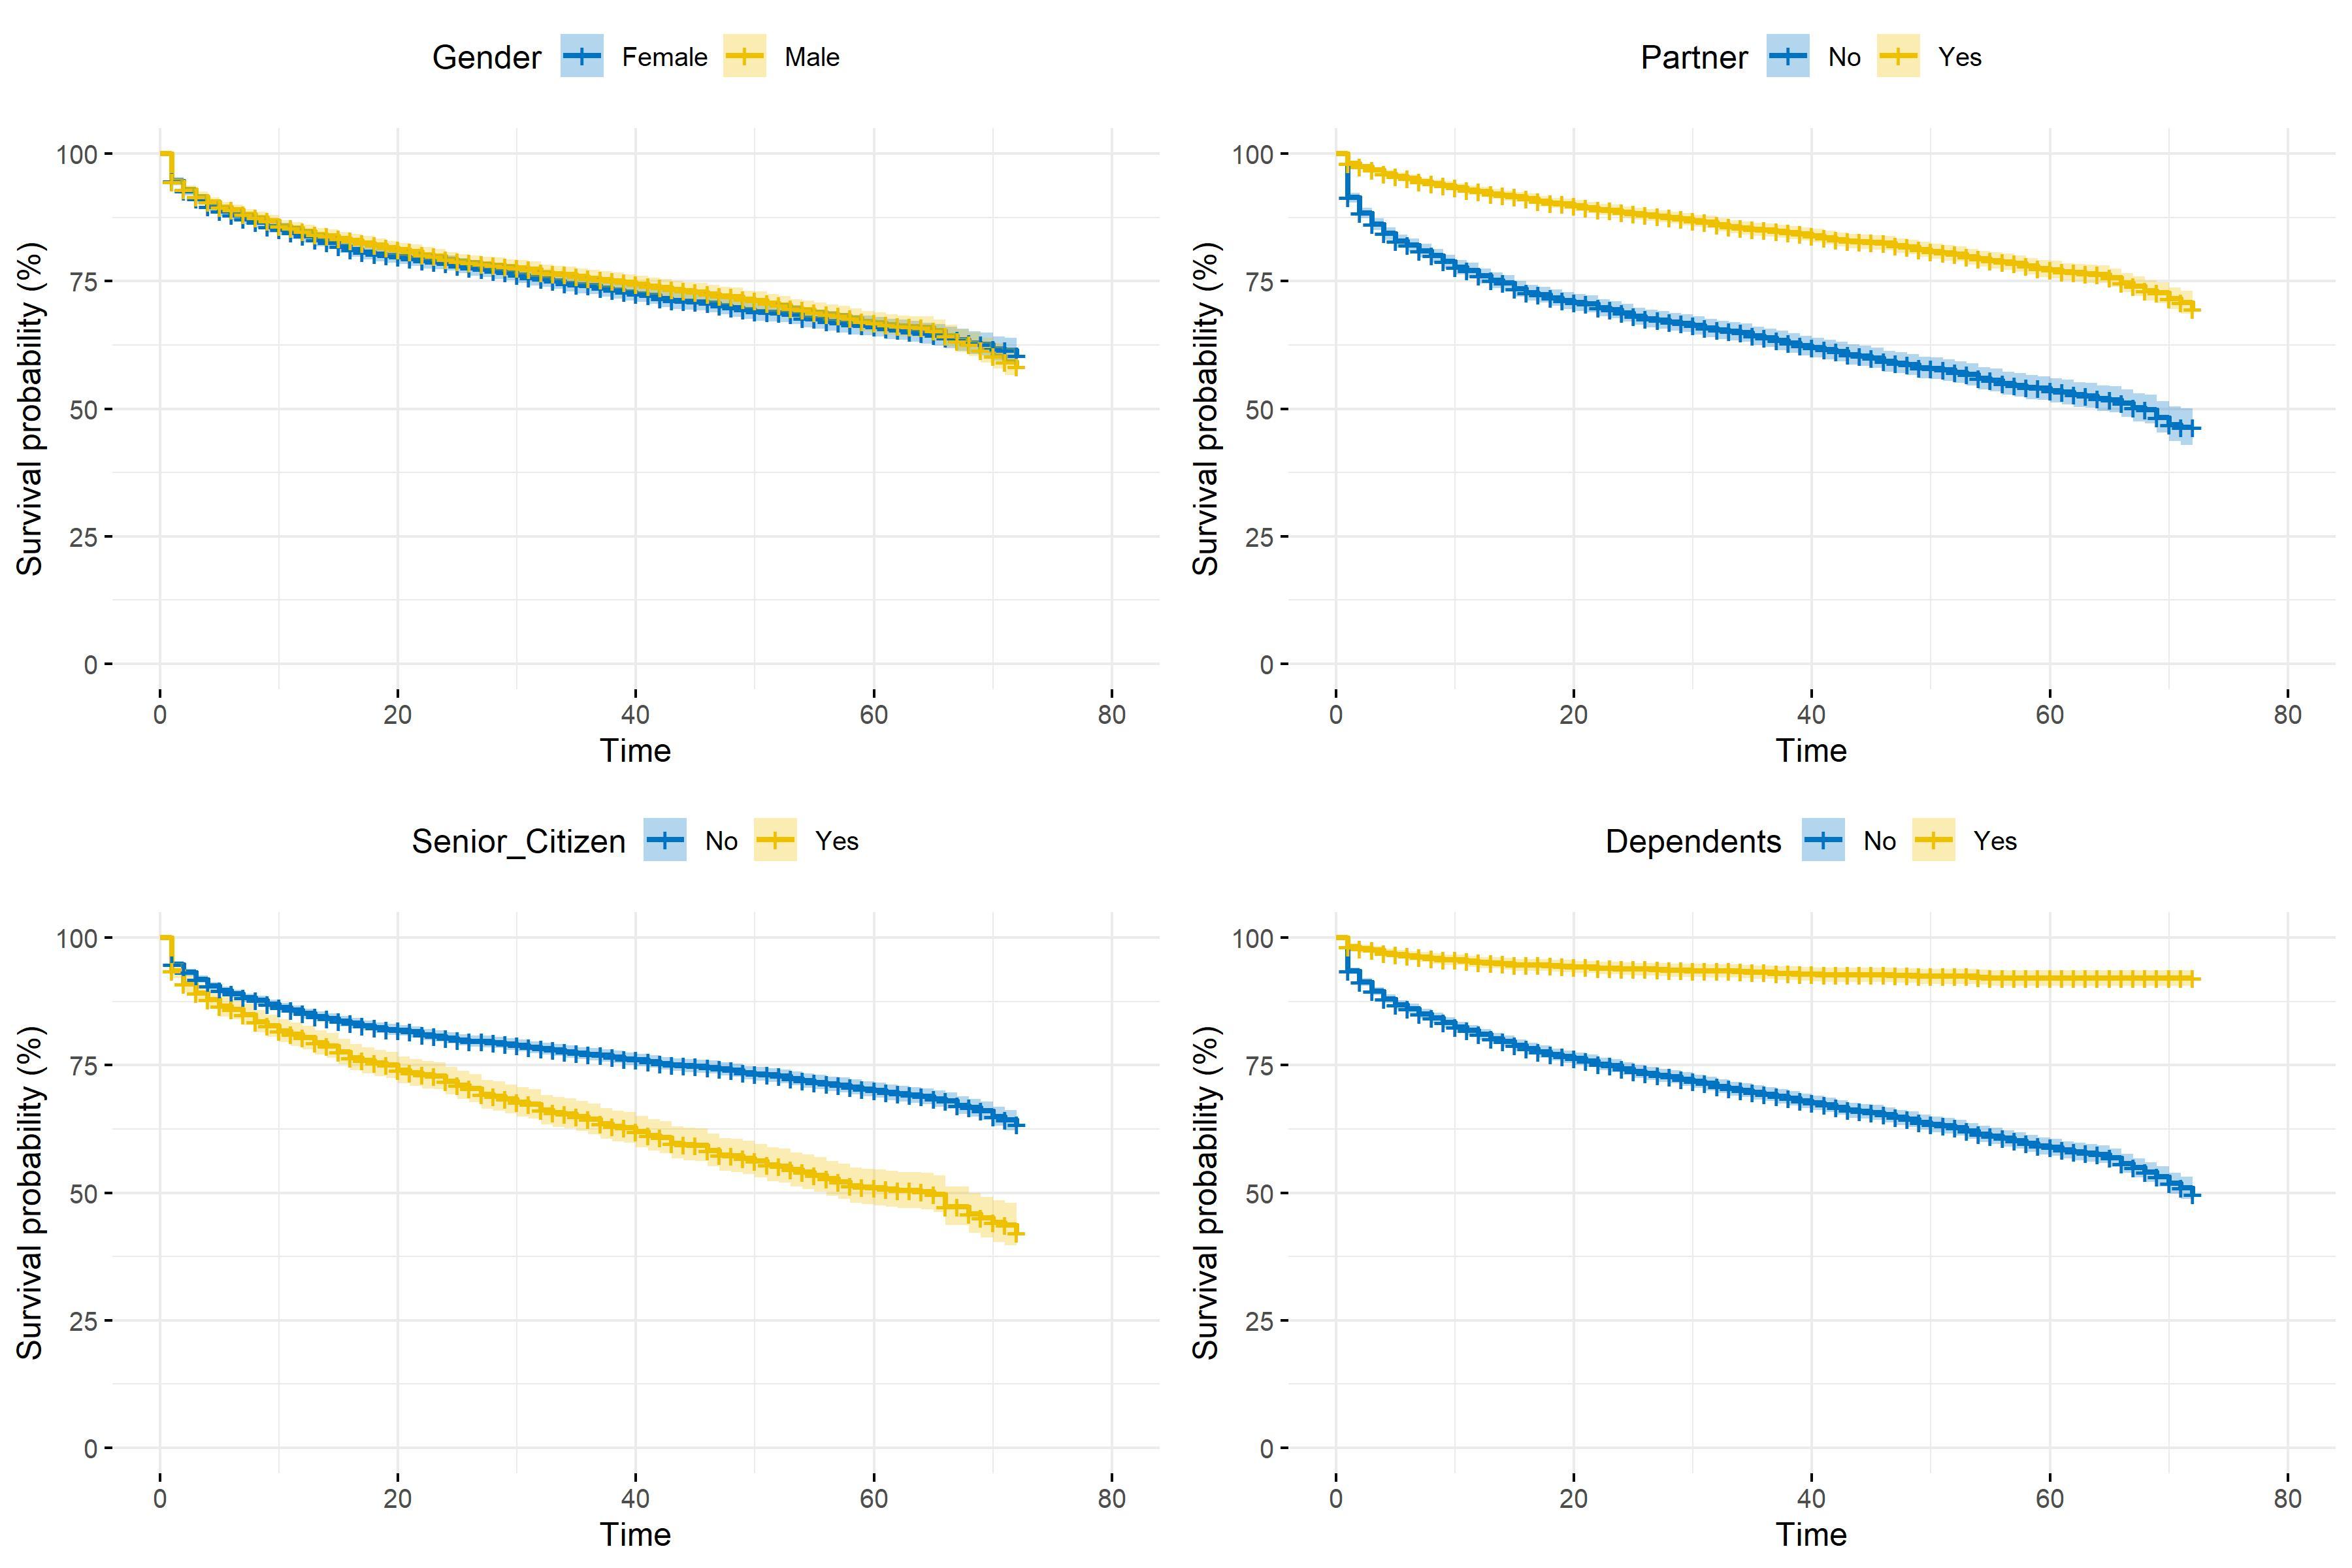
\includegraphics[width=50in]{./imgs/demographics_plot} 

}

\caption{Kaplan-Meier survival function depending on demographic information}\label{fig:kmdemographics}
\end{figure}

\hypertarget{data-on-services-subscribed}{%
\subsection*{Data on services subscribed}\label{data-on-services-subscribed}}
\addcontentsline{toc}{subsection}{Data on services subscribed}

When dealing with data on customers of a TSP, features related to services subscribed may be relevant to explain the estimated survival of these customers in the \emph{portfolio}.

Table \ref{tab:chi2services} presents results of \(\chi^2\) tests performed between \texttt{Churn\_Label} and each services information variable. As in the previous table, \emph{p-values} are ranked in ascending order. One can note that \texttt{Online\_Security} and \texttt{Tech\_Support} are the most linked to the churn indicator variable. However, variable carrying information on phone services are less correlated to \texttt{Churn\_Label}.

\begin{table}[H]

\caption{\label{tab:chi2services}Independence $\chi^2$ test between churn and services information variables}
\centering
\begin{tabular}[t]{lrrrl}
\toprule
  & Statistic & Df & Critical Value & p-value\\
\midrule
\cellcolor{gray!6}{Online\_Security} & \cellcolor{gray!6}{846.68} & \cellcolor{gray!6}{2} & \cellcolor{gray!6}{5.99} & \cellcolor{gray!6}{1.4e-184}\\
Tech\_Support & 824.93 & 2 & 5.99 & 7.4e-180\\
\cellcolor{gray!6}{Internet\_Service} & \cellcolor{gray!6}{728.70} & \cellcolor{gray!6}{2} & \cellcolor{gray!6}{5.99} & \cellcolor{gray!6}{5.8e-159}\\
Online\_Backup & 599.18 & 2 & 5.99 & 7.8e-131\\
\cellcolor{gray!6}{Device\_Protection} & \cellcolor{gray!6}{555.88} & \cellcolor{gray!6}{2} & \cellcolor{gray!6}{5.99} & \cellcolor{gray!6}{2e-121}\\
\addlinespace
Streaming\_Movies & 374.27 & 2 & 5.99 & 5.4e-82\\
\cellcolor{gray!6}{Streaming\_TV} & \cellcolor{gray!6}{372.46} & \cellcolor{gray!6}{2} & \cellcolor{gray!6}{5.99} & \cellcolor{gray!6}{1.3e-81}\\
Multiple\_Lines & 11.27 & 2 & 5.99 & 3.6e-03\\
\cellcolor{gray!6}{Phone\_Service} & \cellcolor{gray!6}{0.87} & \cellcolor{gray!6}{1} & \cellcolor{gray!6}{3.84} & \cellcolor{gray!6}{3.5e-01}\\
\bottomrule
\end{tabular}
\end{table}

Figure \ref{fig:kmservices} illustrates the \(\chi^2\) tests' results by representing the Kaplan-Meier estimated survivor function related to customer lifetime according to treatment variables on services subscribed. On the one hand, there seems to be no significant difference in terms of survival whether the customer uses phone service. The same remark can be pointed out based on whether the client has multiples lines as \texttt{Phone\_Service} and \texttt{Multiple\_Lines} might be quite correlated. In contrast, huge survival time difference can be noticed between customers with online security and those without, as well as between those having subscribed to technical support and those who have not. Finally, not using Internet service appears to have a positive influence on customer lifetime.

\begin{figure}

{\centering 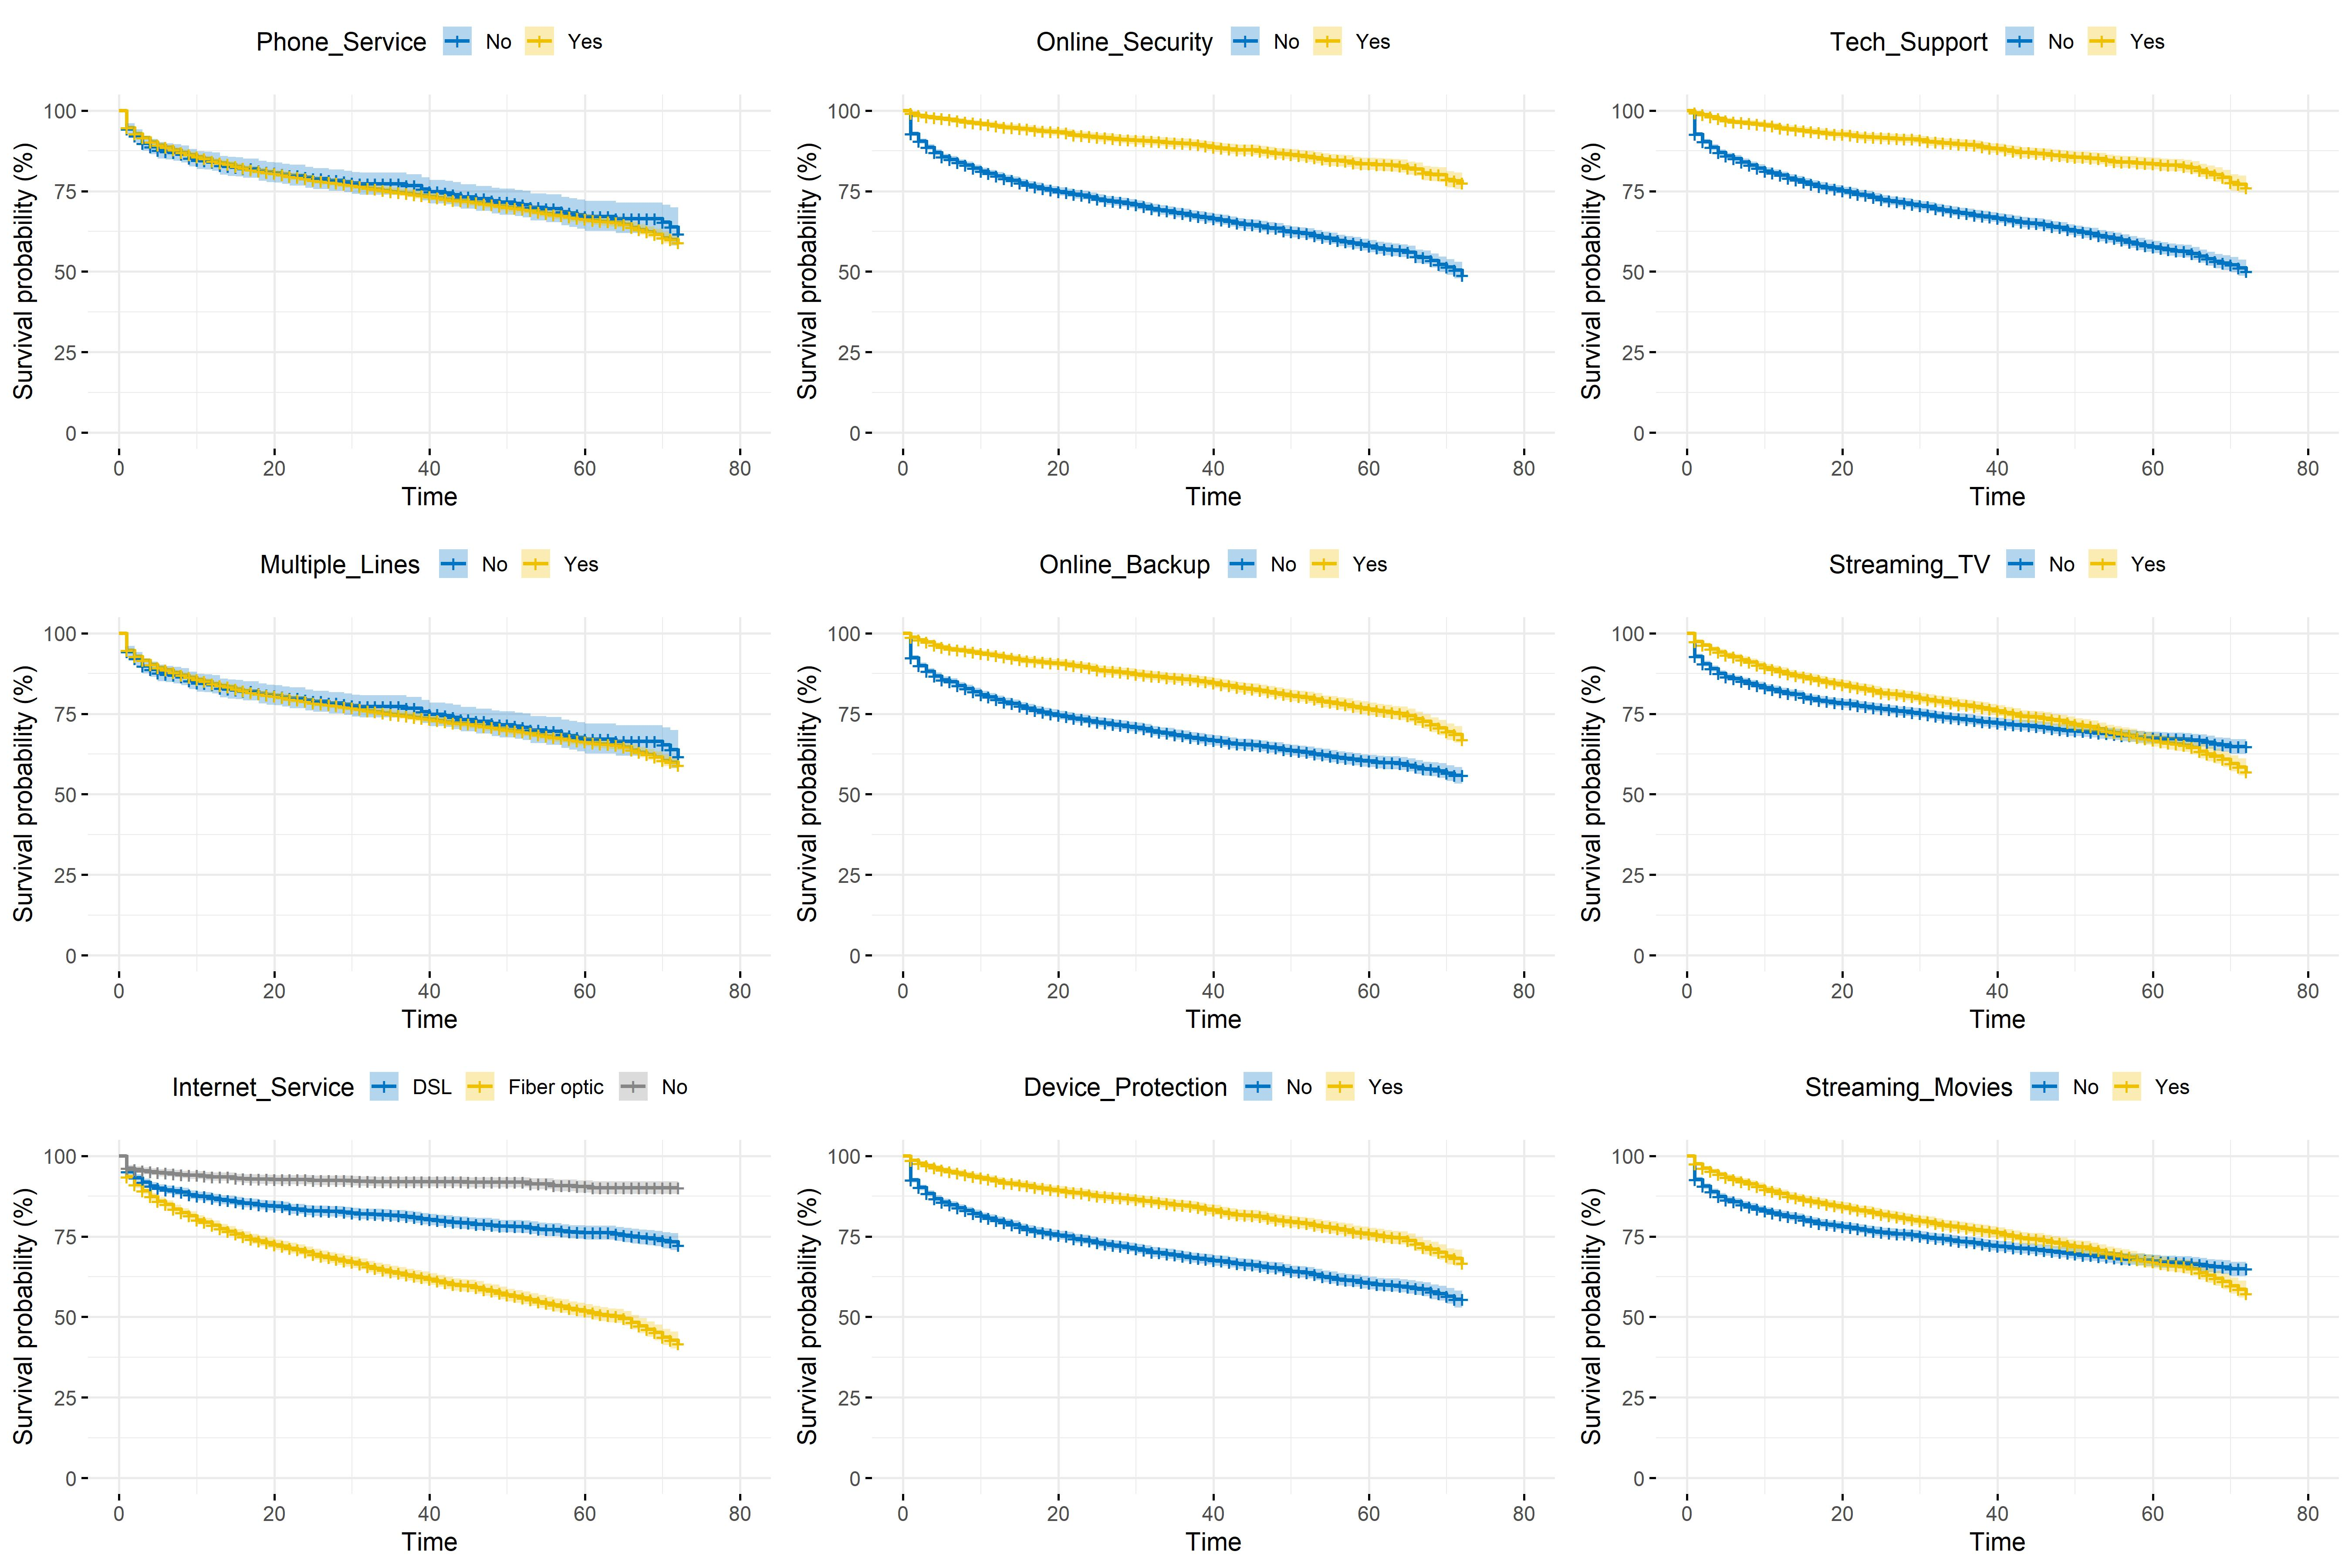
\includegraphics[width=75in]{./imgs/services_plot} 

}

\caption{Kaplan-Meier survival function depending on services subscribed}\label{fig:kmservices}
\end{figure}

\hypertarget{customer-account-data}{%
\subsection*{Customer account data}\label{customer-account-data}}
\addcontentsline{toc}{subsection}{Customer account data}

Variables on customer account such as the payment method used and the type of contract between the TSP and the client can be rich in information in the estimation of customer lifetime. Indeed, table \ref{tab:chi2custaccount} shows that churn status strongly depends on the three variables, \texttt{Contract} being the most linked.

\begin{table}[H]

\caption{\label{tab:chi2custaccount}Independence $\chi^2$ test between churn and customer account data}
\centering
\begin{tabular}[t]{lrrrl}
\toprule
  & Statistic & Df & Critical Value & p-value\\
\midrule
\cellcolor{gray!6}{Contract} & \cellcolor{gray!6}{1179.55} & \cellcolor{gray!6}{2} & \cellcolor{gray!6}{5.99} & \cellcolor{gray!6}{7.3e-257}\\
Payment\_Method & 645.43 & 3 & 7.81 & 1.4e-139\\
\cellcolor{gray!6}{Paperless\_Billing} & \cellcolor{gray!6}{256.87} & \cellcolor{gray!6}{1} & \cellcolor{gray!6}{3.84} & \cellcolor{gray!6}{8.2e-58}\\
\bottomrule
\end{tabular}
\end{table}

Figure \ref{fig:kmcustaccount} enriches the \(\chi^2\) tests' results as it draws survival curves for each treatment variable's categories. When the firm/client contract is type month-to-month, the estimated survivor function decreases far more than for one-year or two-year contracts. In other words, the churn hazard is higher when the contract is renewed each month. This result makes sense as the customer may decide to leave the \emph{portfolio} each month and their are not committed for one or two years. Furthermore, clients with paperless billing contracts are more prone to churn, just like those paying by electronic check. It can be deduce that the \emph{attrition} risk is higher when the payment method is simplified.

\begin{figure}

{\centering 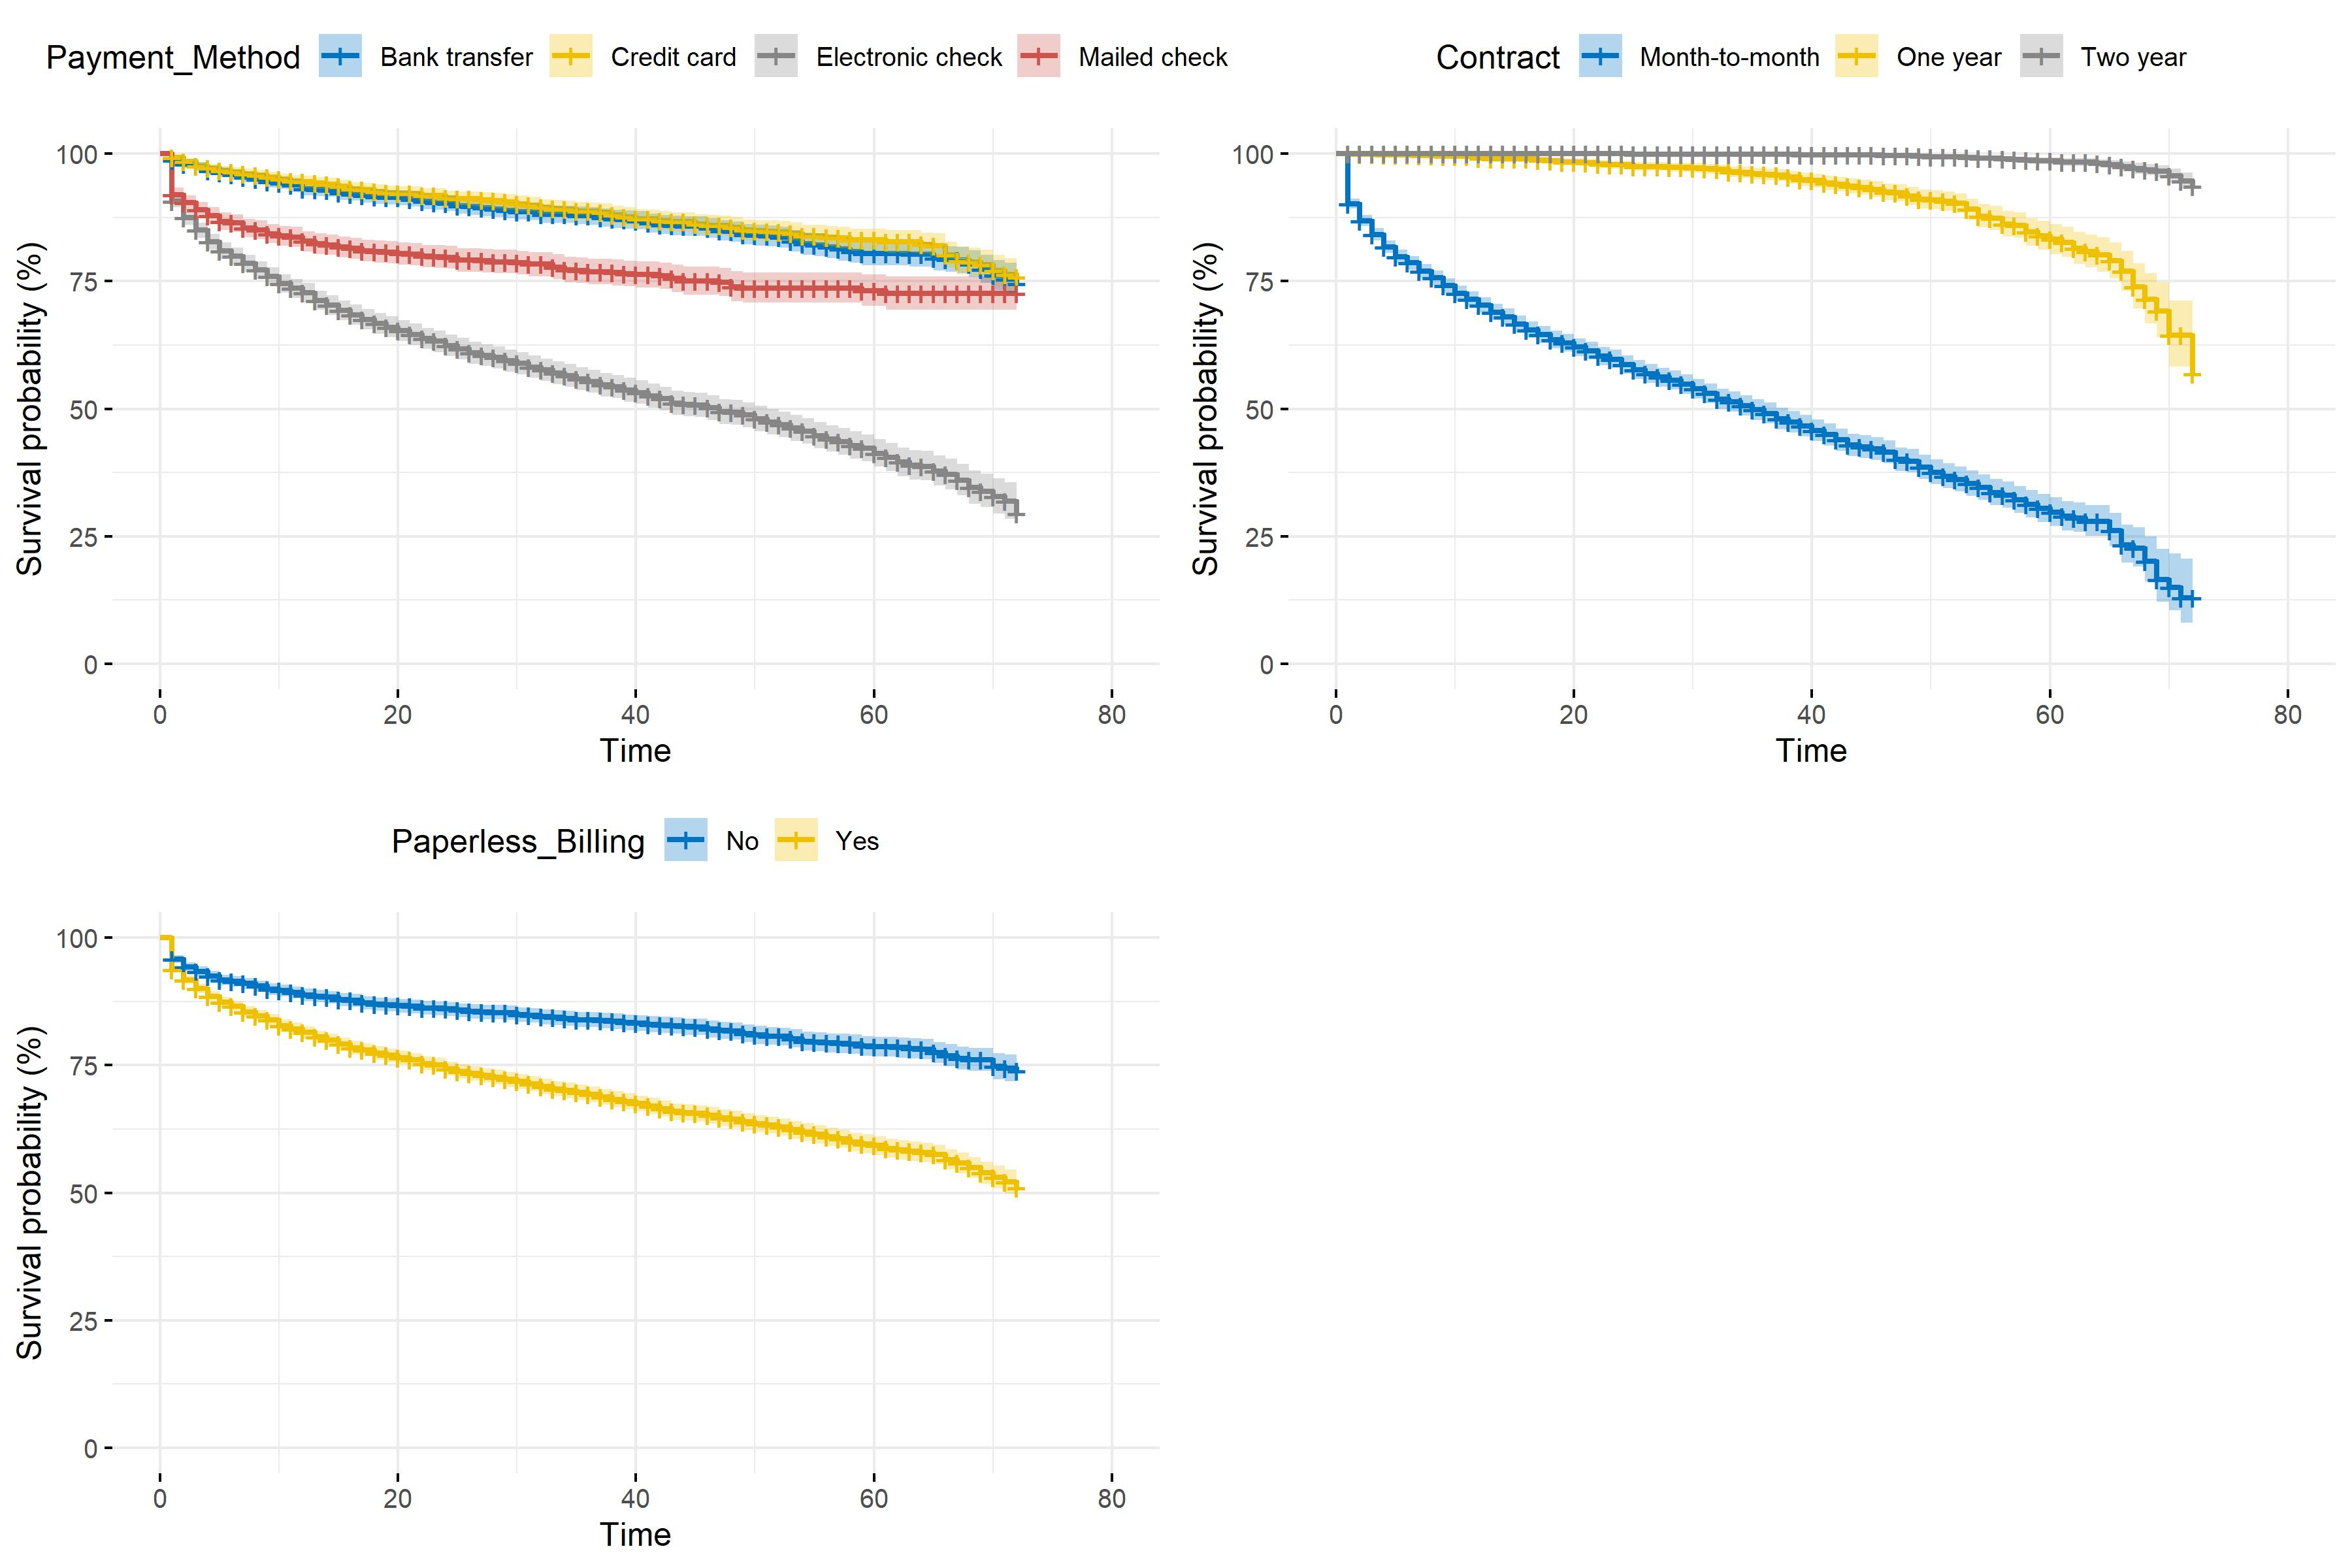
\includegraphics[width=50in]{./imgs/account_info_plot} 

}

\caption{Kaplan-Meier survival function depending on customer account information}\label{fig:kmcustaccount}
\end{figure}

\hypertarget{cltv-customer-lifetime-value}{%
\section{\texorpdfstring{\texttt{CLTV}: Customer Lifetime Value}{CLTV: Customer Lifetime Value}}\label{cltv-customer-lifetime-value}}

In the dataset, the \emph{value} of the fictional TSP's customers is measured by the discrete quantitative variable called \texttt{CLTV}. In this context, it is decided to draw histogram and density plots related to \texttt{CLTV} depending on the three types of explanatory variables. Anova tests are also implemented to verify whether \texttt{CLTV} has different values in the categorical features' different groups. Anova is a generalization of the Student's t test allowing to compare more than two groups. The test's statistic computes the ratio between variance between sample and variance within samples and is Fisher distributed. A low ratio indicates that there is no significant difference between the means of the samples being compared.

\hypertarget{demographic-data-1}{%
\subsection*{Demographic data}\label{demographic-data-1}}
\addcontentsline{toc}{subsection}{Demographic data}

Based on the Anova tests' results, \texttt{Partner} and \texttt{Dependents} seem to be statistically discriminant in terms of customer lifetime value which is not the case for \texttt{Gender} and \texttt{Senior\_Citizen}.

\begin{table}[H]

\caption{\label{tab:aovdemographics}Anova test between CLTV and demographic variables}
\centering
\begin{tabular}[t]{lrrrl}
\toprule
  & F statistic & Df1 & Df2 & p-value\\
\midrule
\cellcolor{gray!6}{Partner} & \cellcolor{gray!6}{139.76} & \cellcolor{gray!6}{1} & \cellcolor{gray!6}{7030} & \cellcolor{gray!6}{6e-32}\\
Dependents & 24.89 & 1 & 7030 & 6.2e-07\\
\cellcolor{gray!6}{Gender} & \cellcolor{gray!6}{0.39} & \cellcolor{gray!6}{1} & \cellcolor{gray!6}{7030} & \cellcolor{gray!6}{5.3e-01}\\
Senior\_Citizen & 0.09 & 1 & 7030 & 7.6e-01\\
\bottomrule
\end{tabular}
\end{table}

The figure below illustrates how different CLV is between customers with a partner and those without, as well as between those with children o other dependants and those without. To put it another way, having a partner in life of dependants tends to increase customer lifetime value as shown by the two last histograms.

\begin{figure}

{\centering 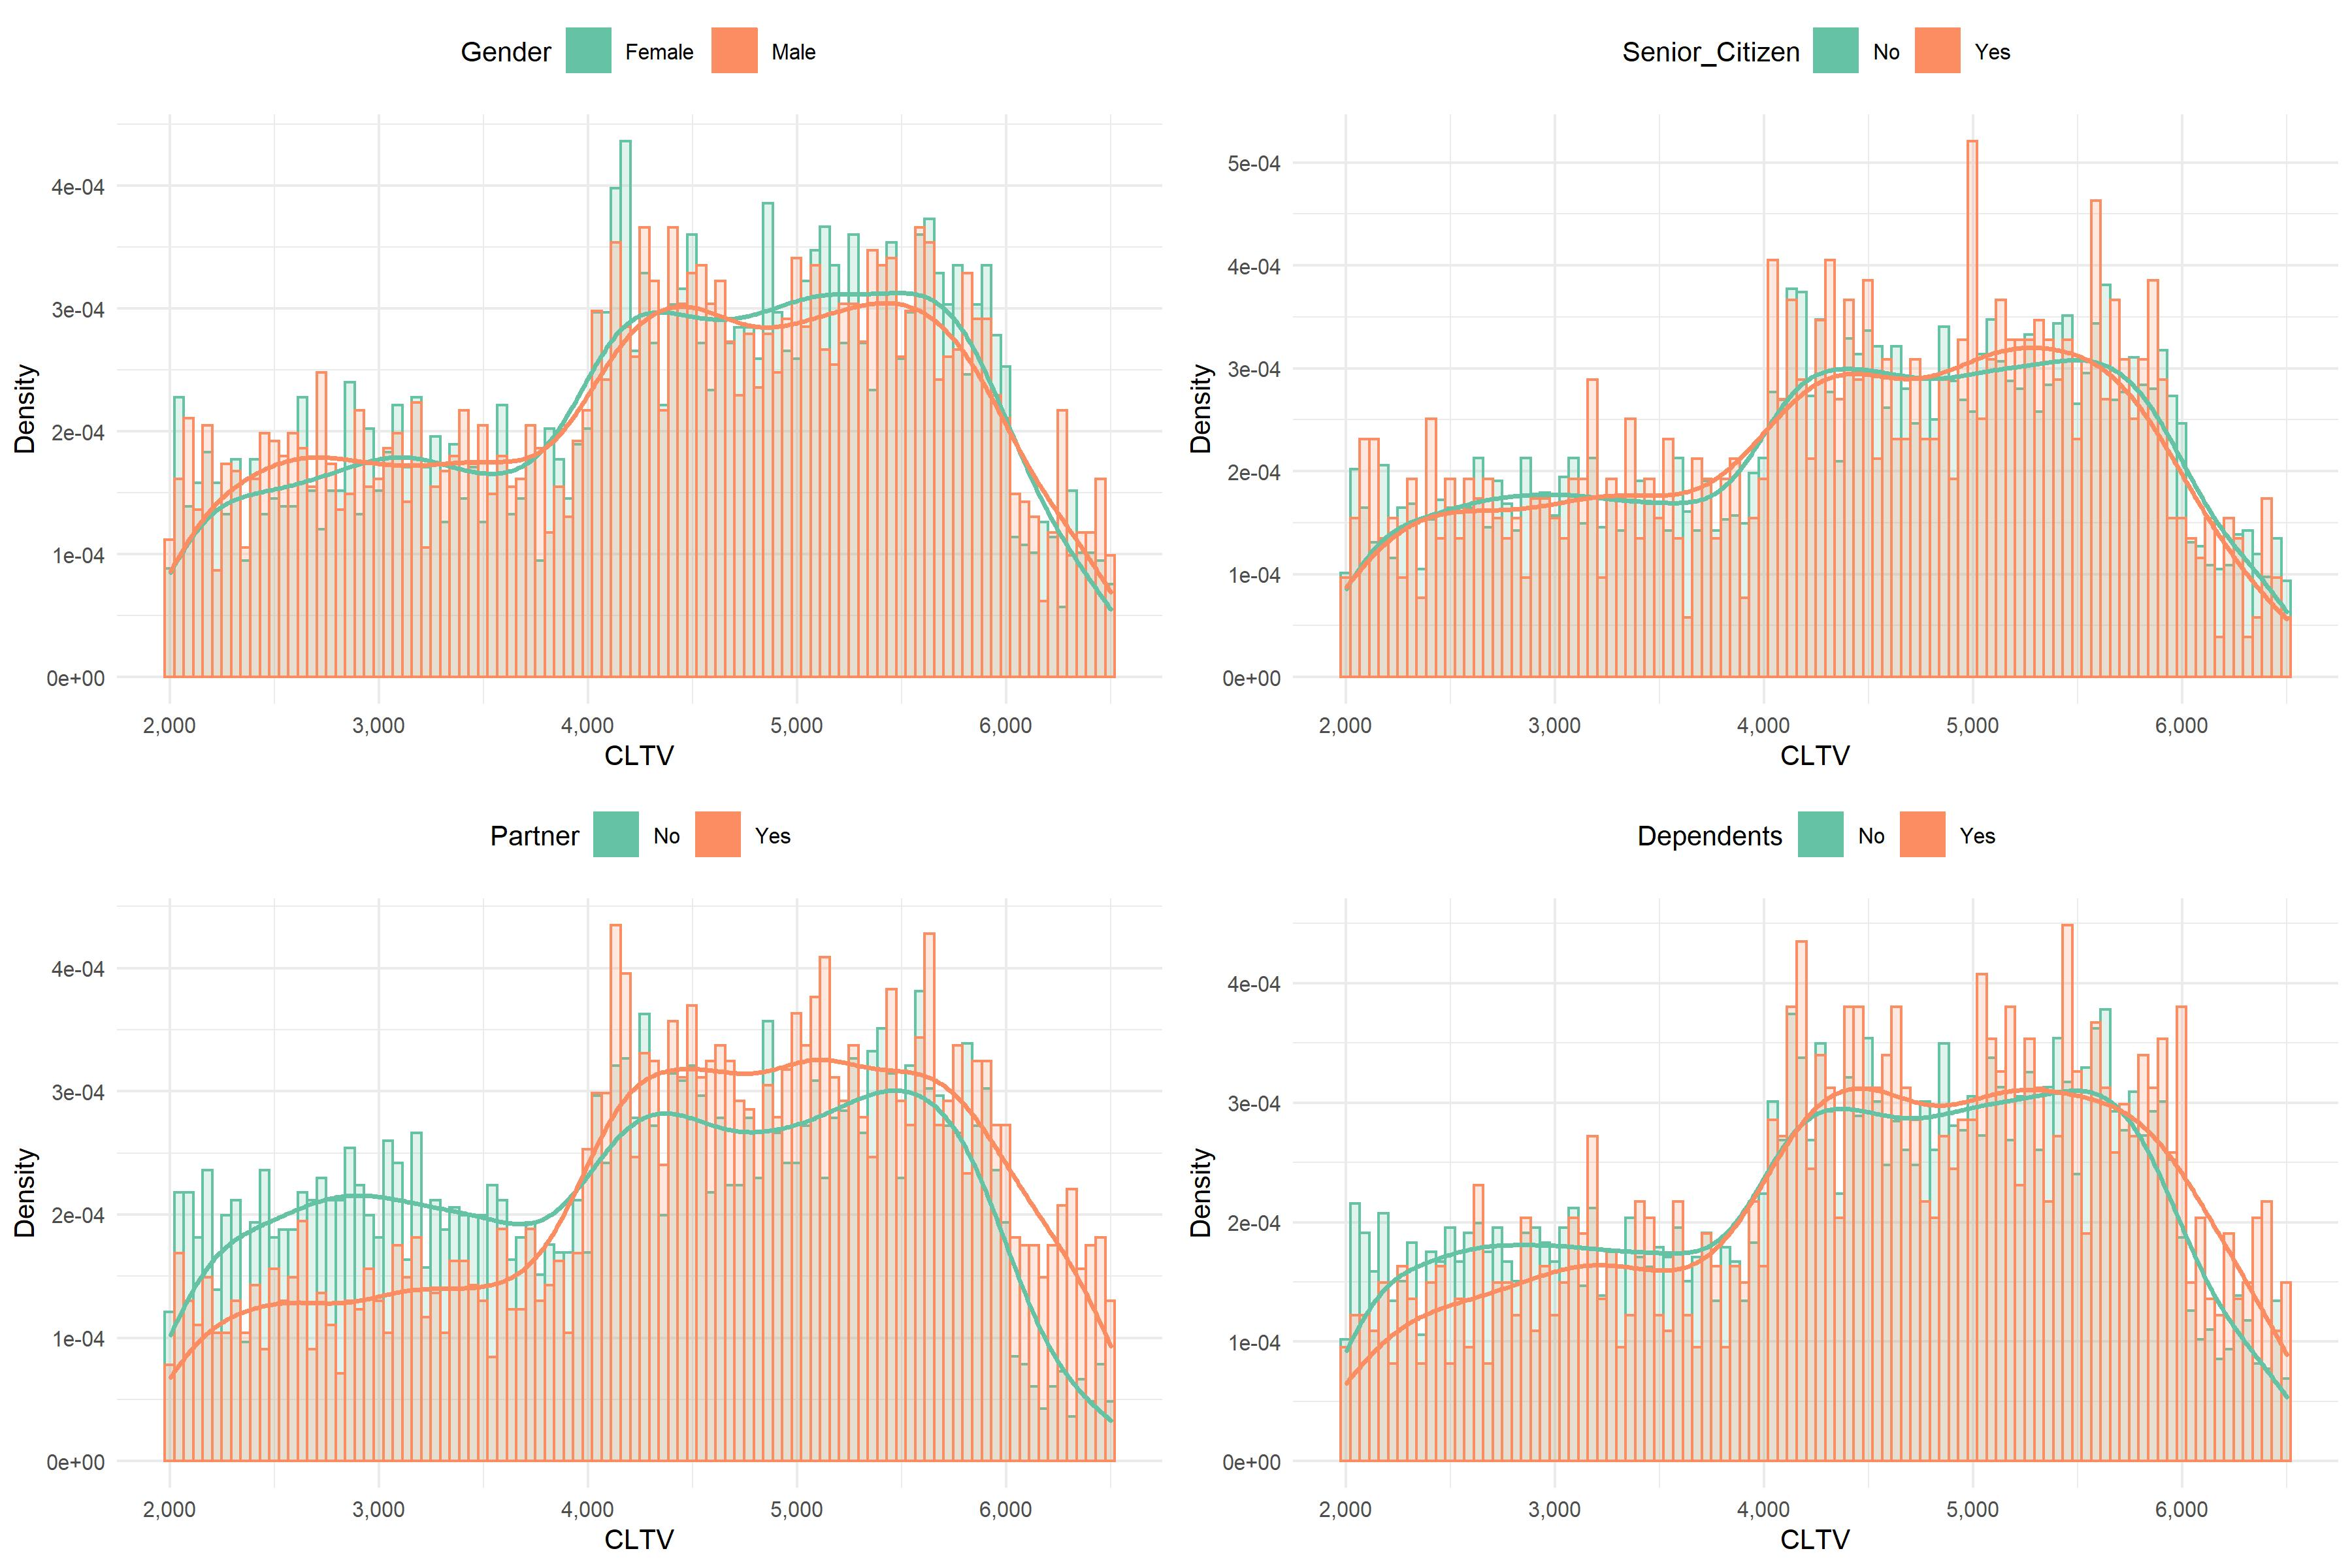
\includegraphics[width=50in]{./imgs/cltv_demographics_plots} 

}

\caption{Histogram and density plots of customer lifetime value depending on demographic information}\label{fig:cltvdemographics}
\end{figure}

\hypertarget{data-on-services-subscribed-1}{%
\subsection*{Data on services subscribed}\label{data-on-services-subscribed-1}}
\addcontentsline{toc}{subsection}{Data on services subscribed}

When on wants to identify factors influencing customer lifetime value, it is relevant to consider variables related to services subscribed by customers. The Anova tests' results indicate that \texttt{CLTV} has significant different values in each group of all services related variables, except for \texttt{Internet\_Service}. The most important different can be noted for \texttt{Online\_Backup} and \texttt{Online\_Security} variables, whereas there is more homogeneity in the \texttt{Phone\_Service} groups.

\begin{table}[H]

\caption{\label{tab:aovservices}Anova test between CLTV and services information variables}
\centering
\begin{tabular}[t]{lrrrl}
\toprule
  & F statistic & Df1 & Df2 & p-value\\
\midrule
\cellcolor{gray!6}{Online\_Backup} & \cellcolor{gray!6}{76.75} & \cellcolor{gray!6}{2} & \cellcolor{gray!6}{7029} & \cellcolor{gray!6}{1.1e-33}\\
Online\_Security & 74.14 & 2 & 7029 & 1.4e-32\\
\cellcolor{gray!6}{Multiple\_Lines} & \cellcolor{gray!6}{64.81} & \cellcolor{gray!6}{2} & \cellcolor{gray!6}{7029} & \cellcolor{gray!6}{1.3e-28}\\
Device\_Protection & 57.79 & 2 & 7029 & 1.3e-25\\
\cellcolor{gray!6}{Tech\_Support} & \cellcolor{gray!6}{54.33} & \cellcolor{gray!6}{2} & \cellcolor{gray!6}{7029} & \cellcolor{gray!6}{3.8e-24}\\
\addlinespace
Streaming\_Movies & 51.18 & 2 & 7029 & 8.6e-23\\
\cellcolor{gray!6}{Streaming\_TV} & \cellcolor{gray!6}{44.43} & \cellcolor{gray!6}{2} & \cellcolor{gray!6}{7029} & \cellcolor{gray!6}{6.7e-20}\\
Phone\_Service & 3.65 & 1 & 7030 & 5.6e-02\\
\cellcolor{gray!6}{Internet\_Service} & \cellcolor{gray!6}{0.56} & \cellcolor{gray!6}{2} & \cellcolor{gray!6}{7029} & \cellcolor{gray!6}{5.7e-01}\\
\bottomrule
\end{tabular}
\end{table}

From figure \ref{fig:cltvservices} one can note that subscribing to additional services like having multiple lines, online security and backup, device protection or using the streaming movie service significantly enhance customer lifetime value. These variables may be interesting predictor of the \texttt{CLTV} in regression models.

\begin{figure}

{\centering 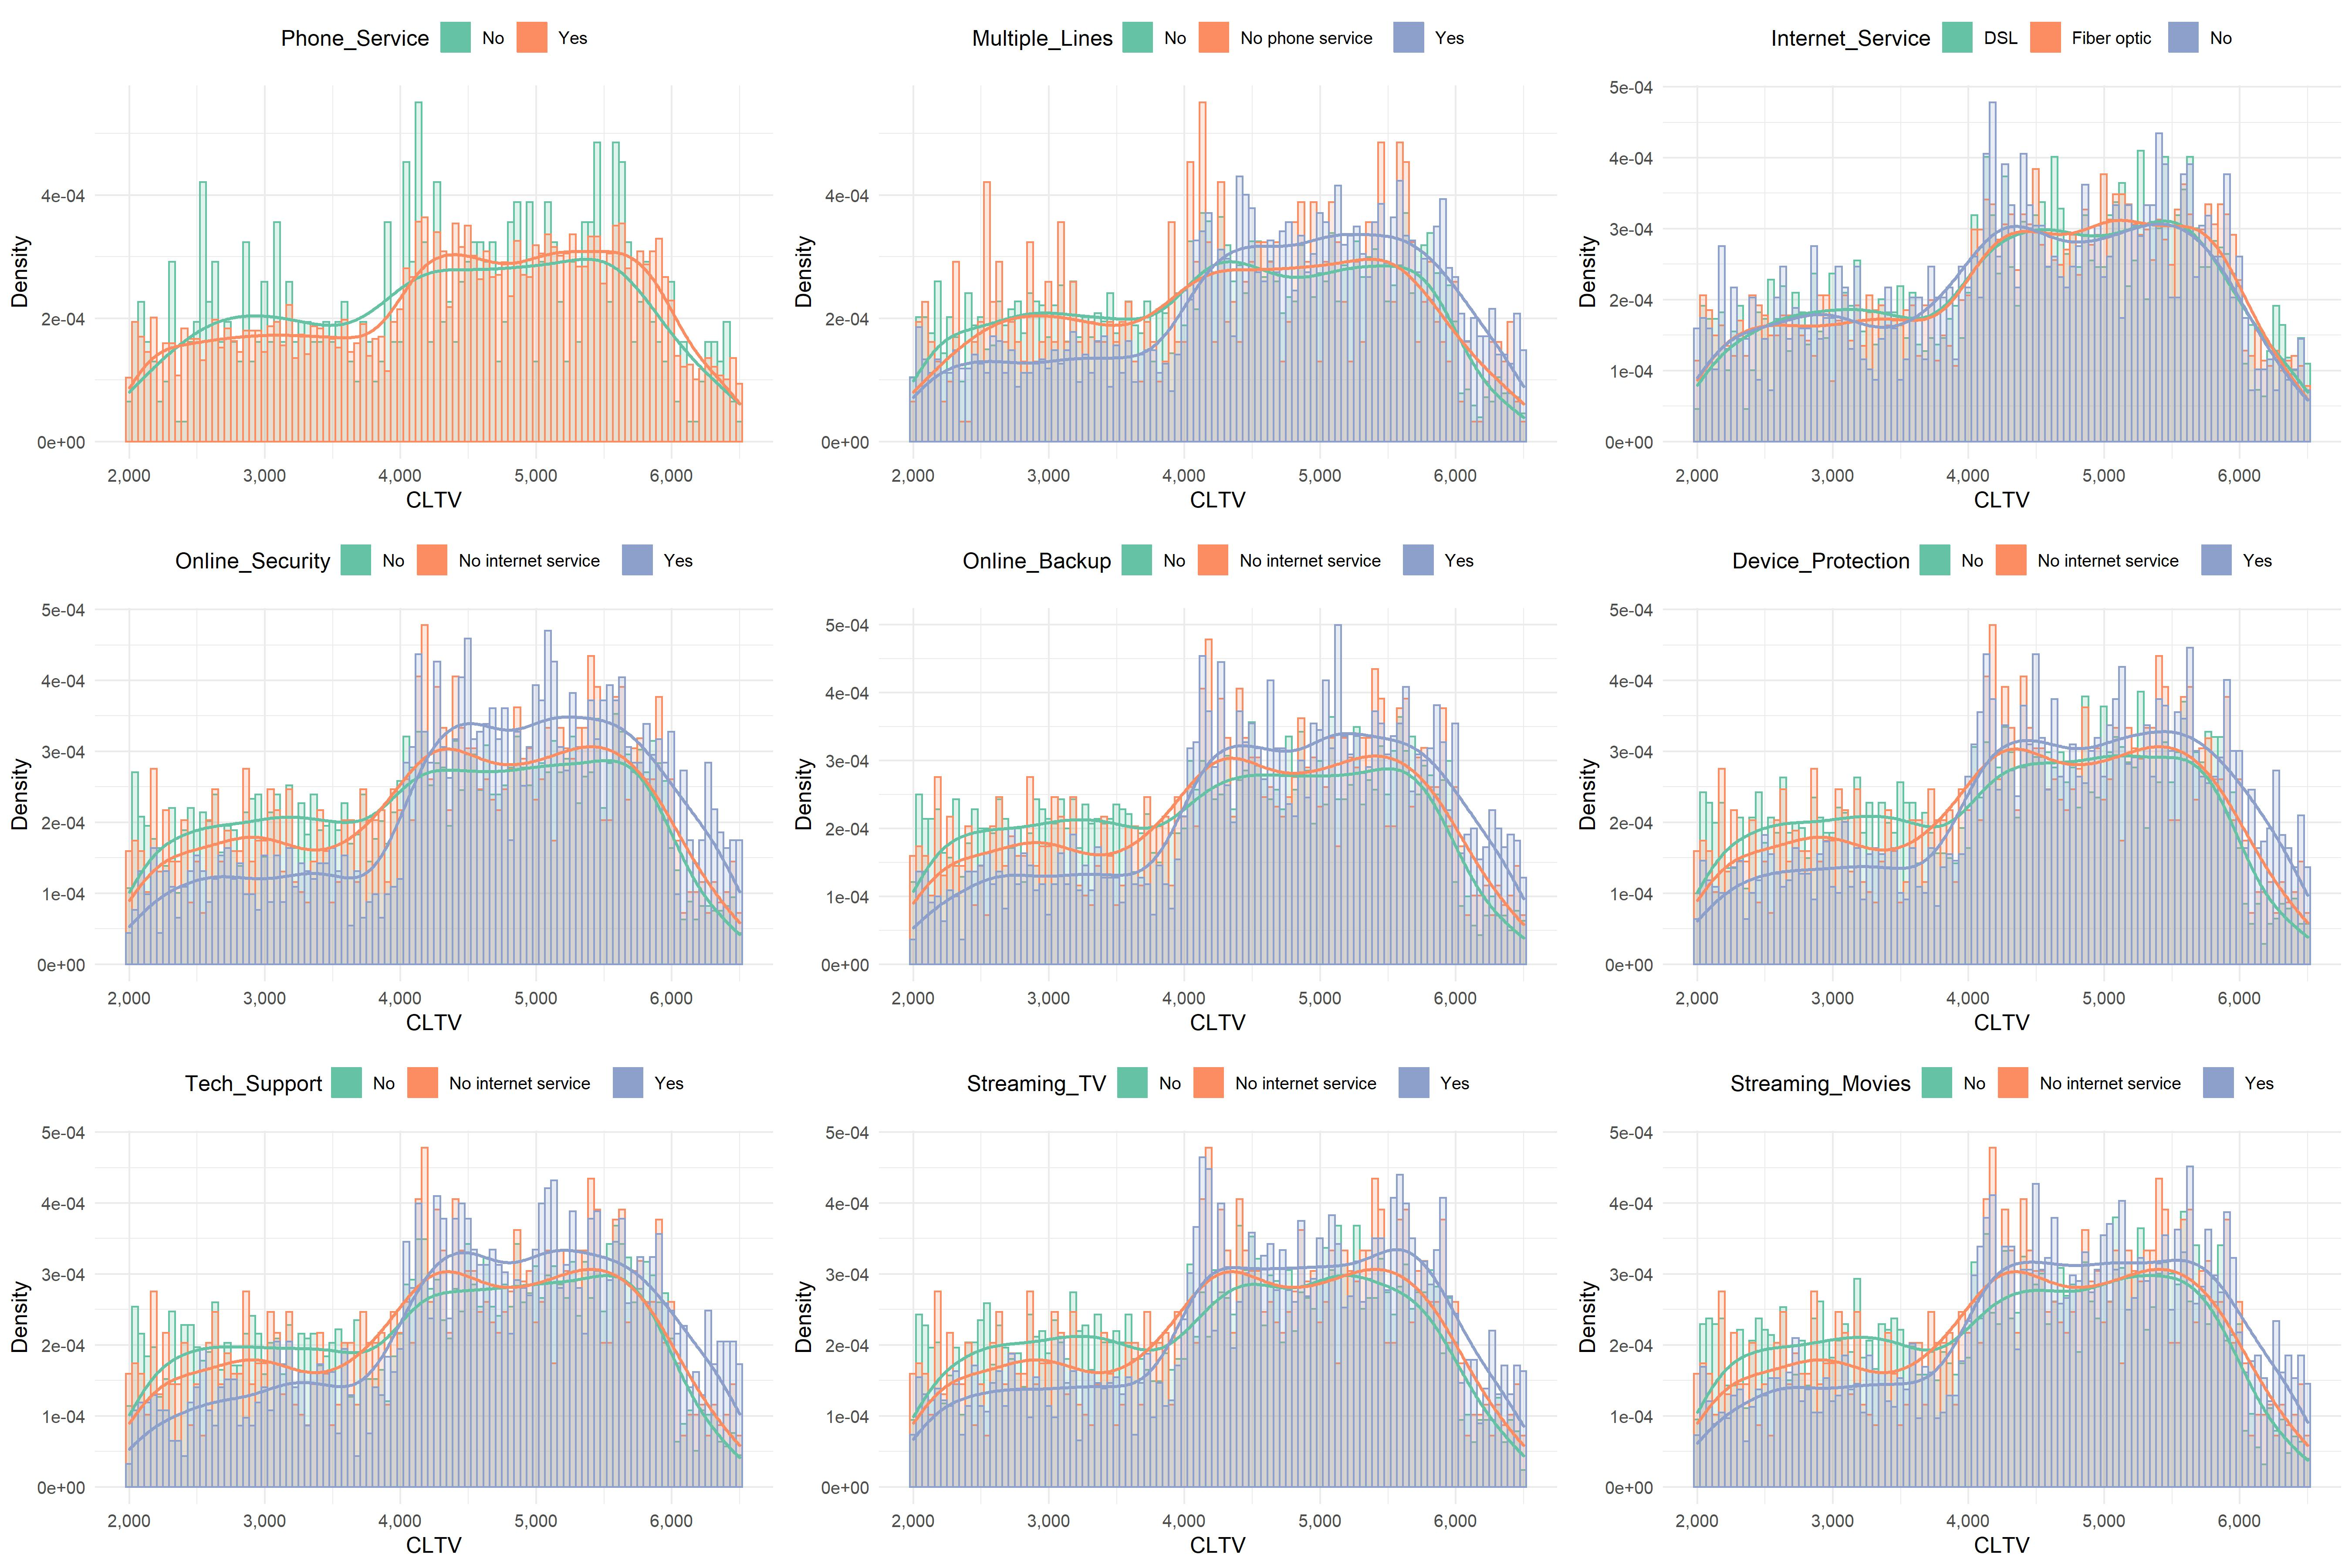
\includegraphics[width=75in]{./imgs/cltv_services_plots} 

}

\caption{Histogram and density plots of customer lifetime value depending on services subscribed}\label{fig:cltvservices}
\end{figure}

\hypertarget{customer-account-data-1}{%
\subsection*{Customer account data}\label{customer-account-data-1}}
\addcontentsline{toc}{subsection}{Customer account data}

Table \ref{tab:aovaccountinfo} depicts that \texttt{CLTV} is statistically different according to the type of contract and the payment method. However, paperless billing does not seem to influence customer lifetime value.

\begin{table}[H]

\caption{\label{tab:aovaccountinfo}Anova test between CLTV and customer account data}
\centering
\begin{tabular}[t]{lrrrl}
\toprule
  & F statistic & Df1 & Df2 & p-value\\
\midrule
\cellcolor{gray!6}{Contract} & \cellcolor{gray!6}{274.28} & \cellcolor{gray!6}{2} & \cellcolor{gray!6}{7029} & \cellcolor{gray!6}{2e-115}\\
Payment\_Method & 52.66 & 3 & 7028 & 1.2e-33\\
\cellcolor{gray!6}{Paperless\_Billing} & \cellcolor{gray!6}{0.77} & \cellcolor{gray!6}{1} & \cellcolor{gray!6}{7030} & \cellcolor{gray!6}{3.8e-01}\\
\bottomrule
\end{tabular}
\end{table}

The three plots below provide details to previous results as it can be noticed that customers paying by credit card of bank transfer have higher CLV than those paying by e-check of mailed check. Besides, clients enrolled in one-year or two-year contracts have greater \emph{value} to thefirm than those who pay on a monthly basis.

\begin{figure}

{\centering 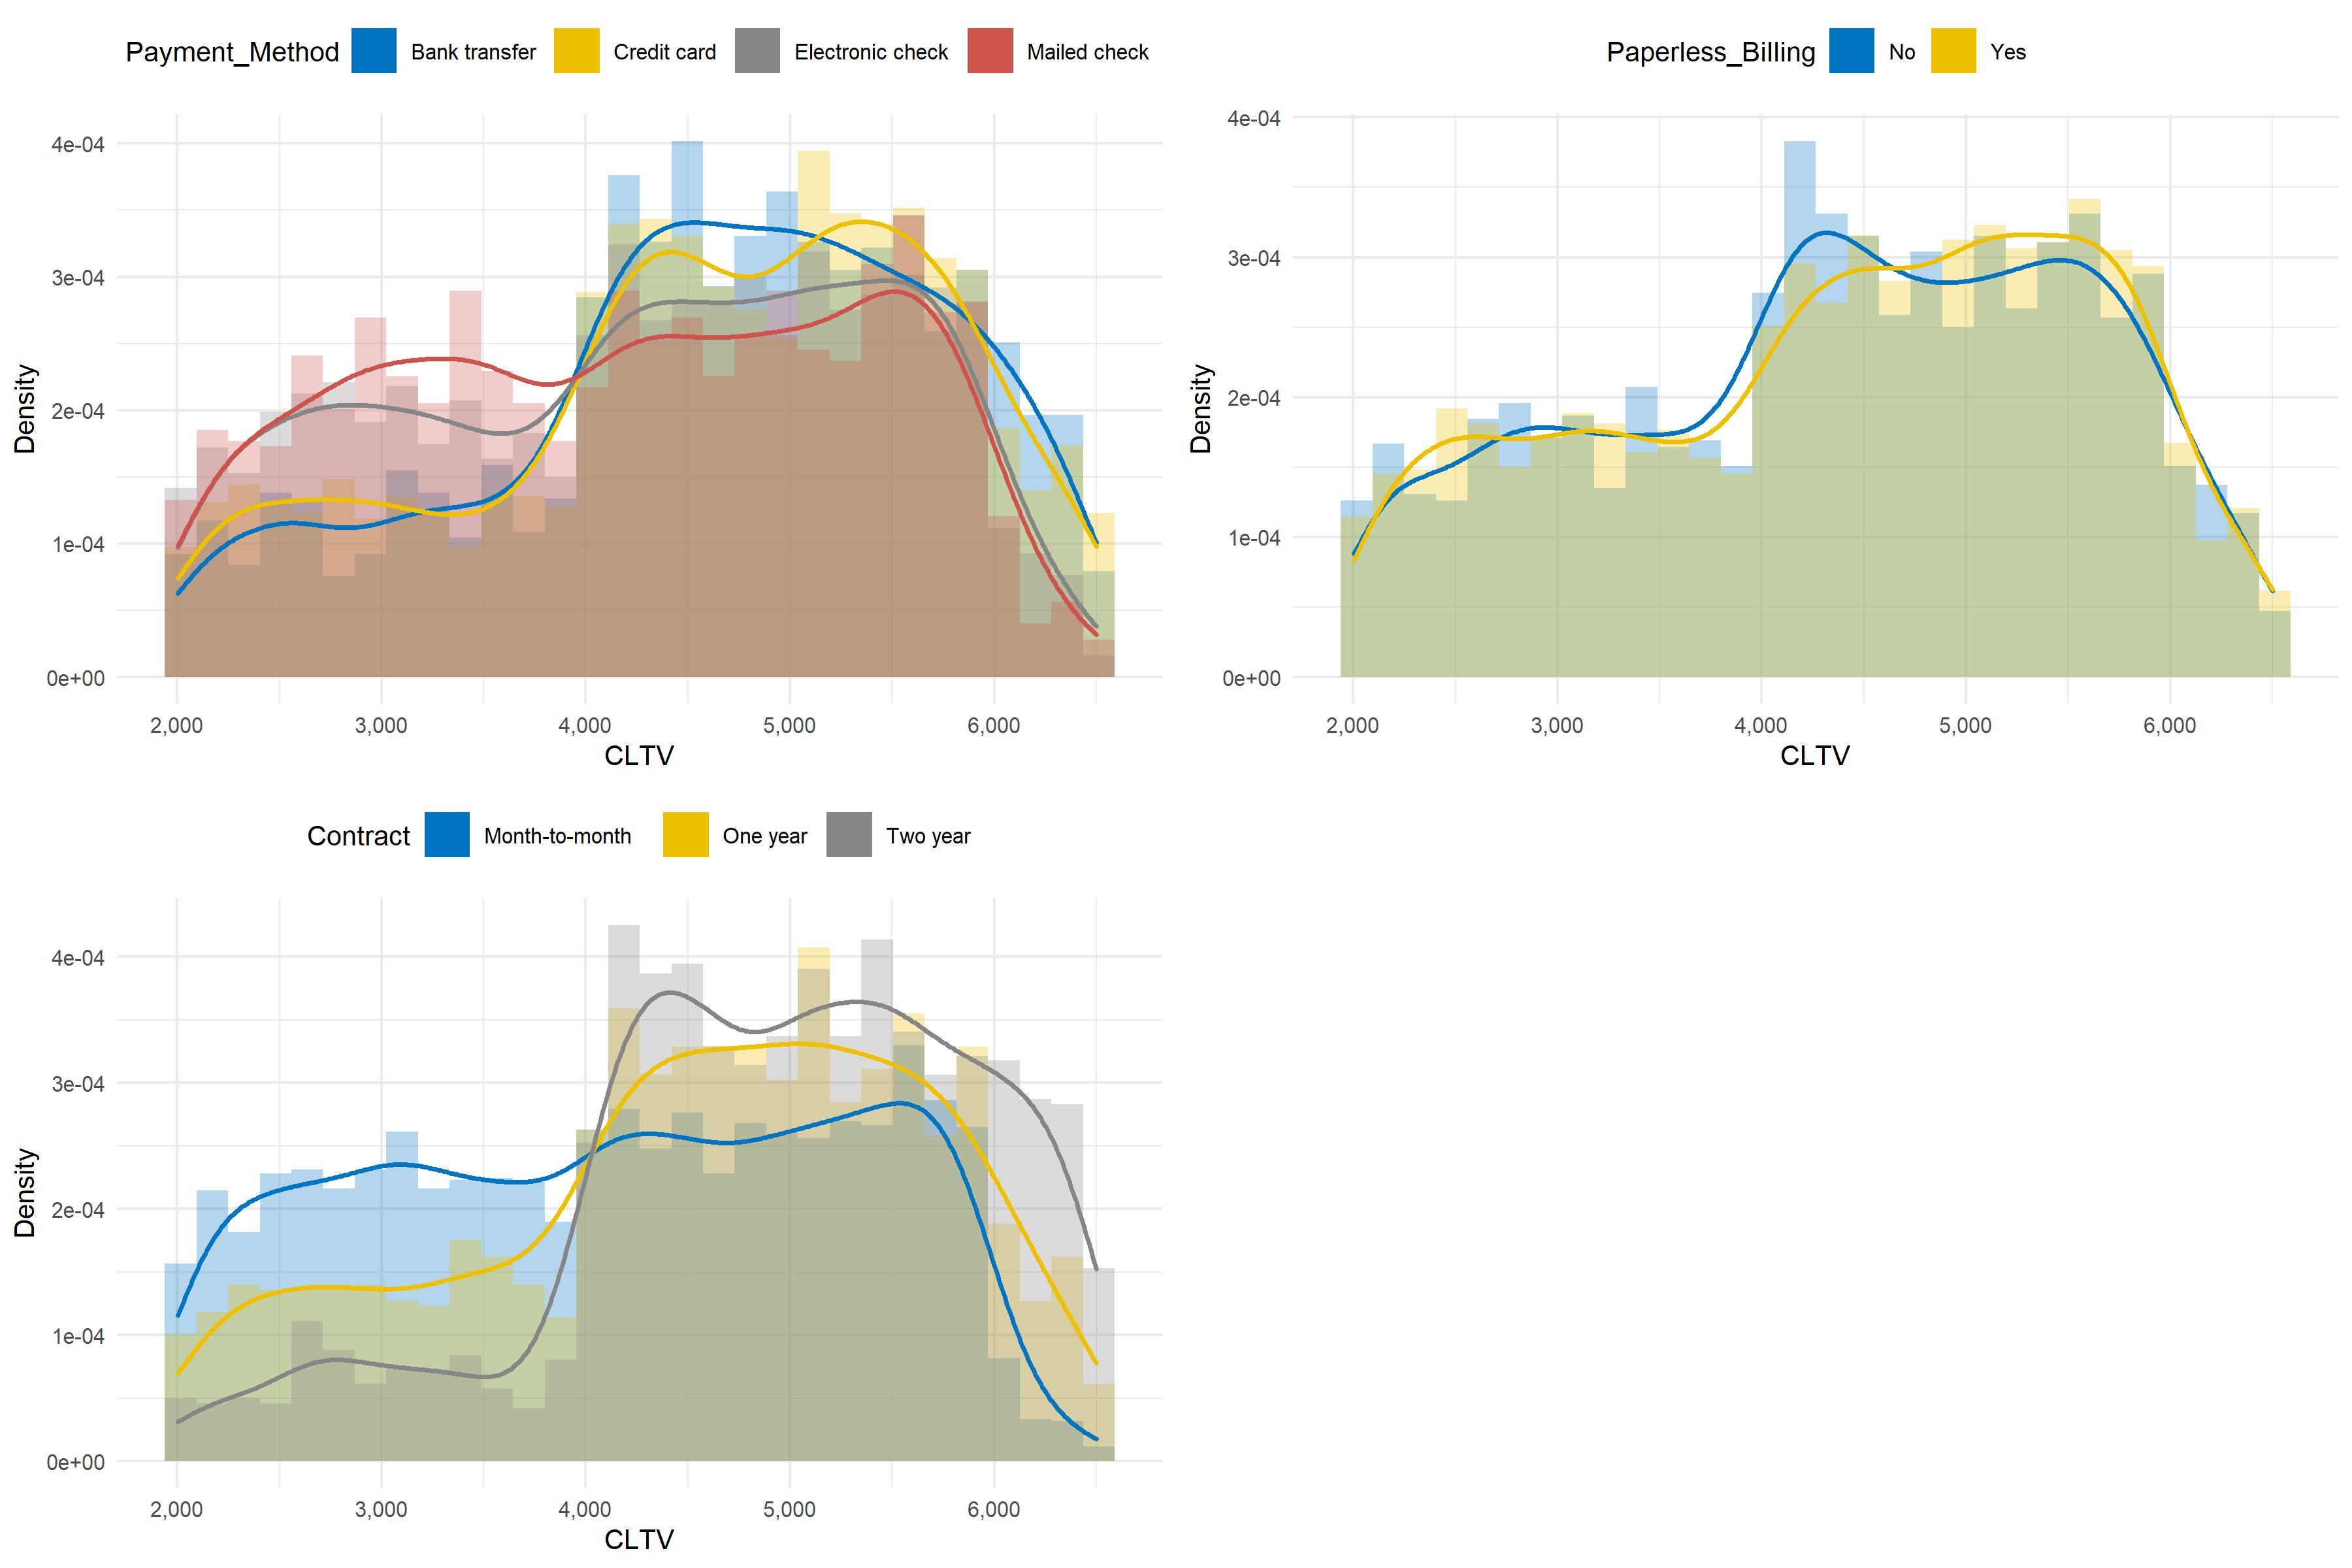
\includegraphics[width=50in]{./imgs/cltv_account_info_plots} 

}

\caption{Histogram and density plots of customer lifetime value depending on customer account data}\label{fig:cltvaccountinfo}
\end{figure}

\hypertarget{correlation-between-cltv-and-explanatory-quantitative-variables}{%
\subsection*{\texorpdfstring{Correlation between \texttt{CLTV} and explanatory quantitative variables}{Correlation between CLTV and explanatory quantitative variables}}\label{correlation-between-cltv-and-explanatory-quantitative-variables}}
\addcontentsline{toc}{subsection}{Correlation between \texttt{CLTV} and explanatory quantitative variables}

Plotting the correlation matrix allows to have an overview on the links between the dataset's quantitative variables. The method used is the Pearson correlation coefficient which is defined as follows:

\begin{equation}
  \rho_{XY} = \frac{\text{cov}(X, Y)}{\sigma_X \sigma_Y}
  \label{eq:pearson}
\end{equation}

where \(X\) and \(Y\) are two quantitative random variables, \(\text{cov}\) the covariance function and \(\sigma\) the standard deviation.

On figure \ref{fig:corrplot}, non-significant correlations are crossed-out. It can be noticed that \texttt{CLTV} has the strongest correlation with \texttt{Tenure\_Months} (\(40\%\)), followed by \texttt{Total\_Charges} (\(34\%\)) then \texttt{Monthly\_Charges} (\(10\%\)).

\begin{figure}

{\centering 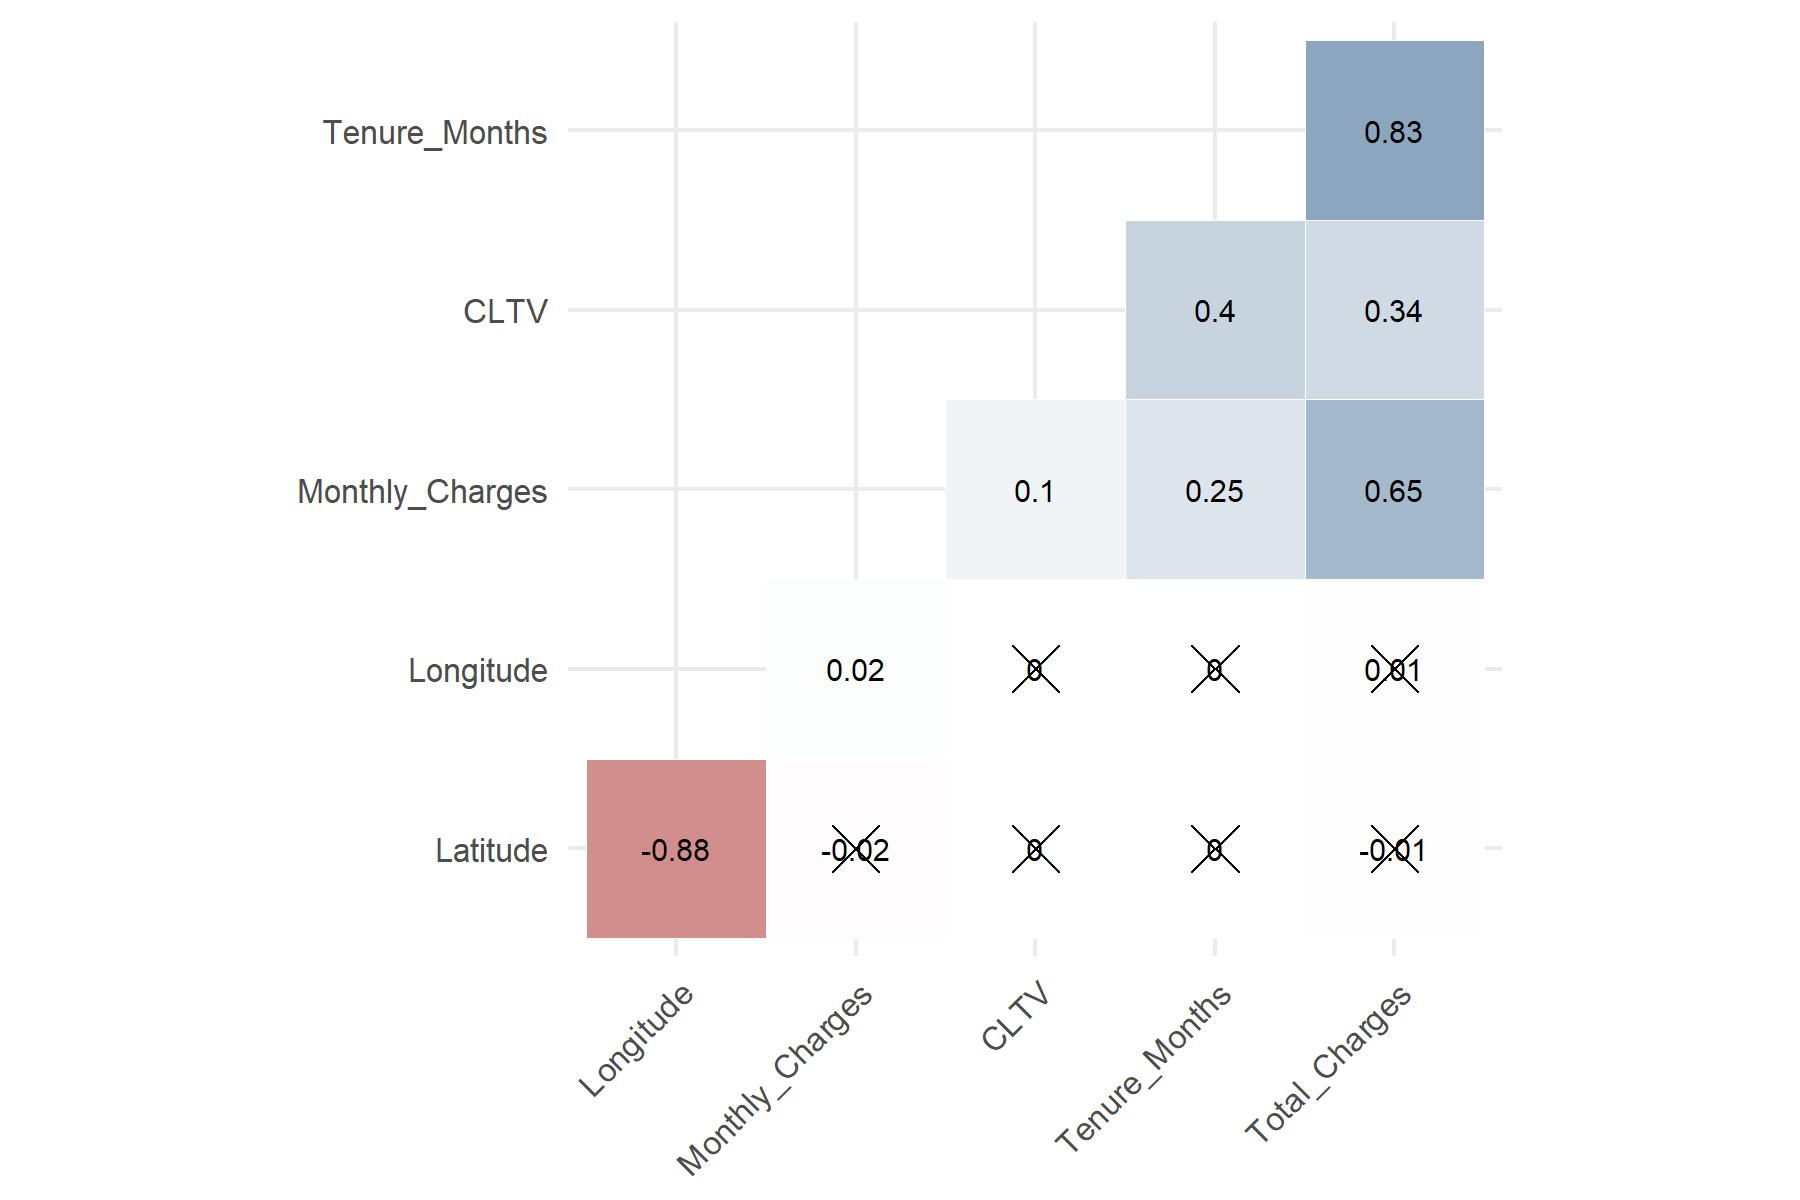
\includegraphics[width=25in]{./imgs/corr_plot} 

}

\caption{Correlation plot}\label{fig:corrplot}
\end{figure}

\hypertarget{churn-duration-and-customer-value}{%
\section{\texorpdfstring{Churn, duration and customer \emph{value}}{Churn, duration and customer value}}\label{churn-duration-and-customer-value}}

The final step in the data exploration consists in analyzing the relationship between the three target variables: \texttt{CLTV}, \texttt{Churn\_Label} and \texttt{Tenure\_Months}.

Looking at figure \ref{fig:cltvchurn}, customer lifetime value seems to have higher values for retained customers than for churners as the density is more right-oriented. This result makes sense as retained customers may have longer lifetime leading to higgher CLV.

\begin{figure}

{\centering 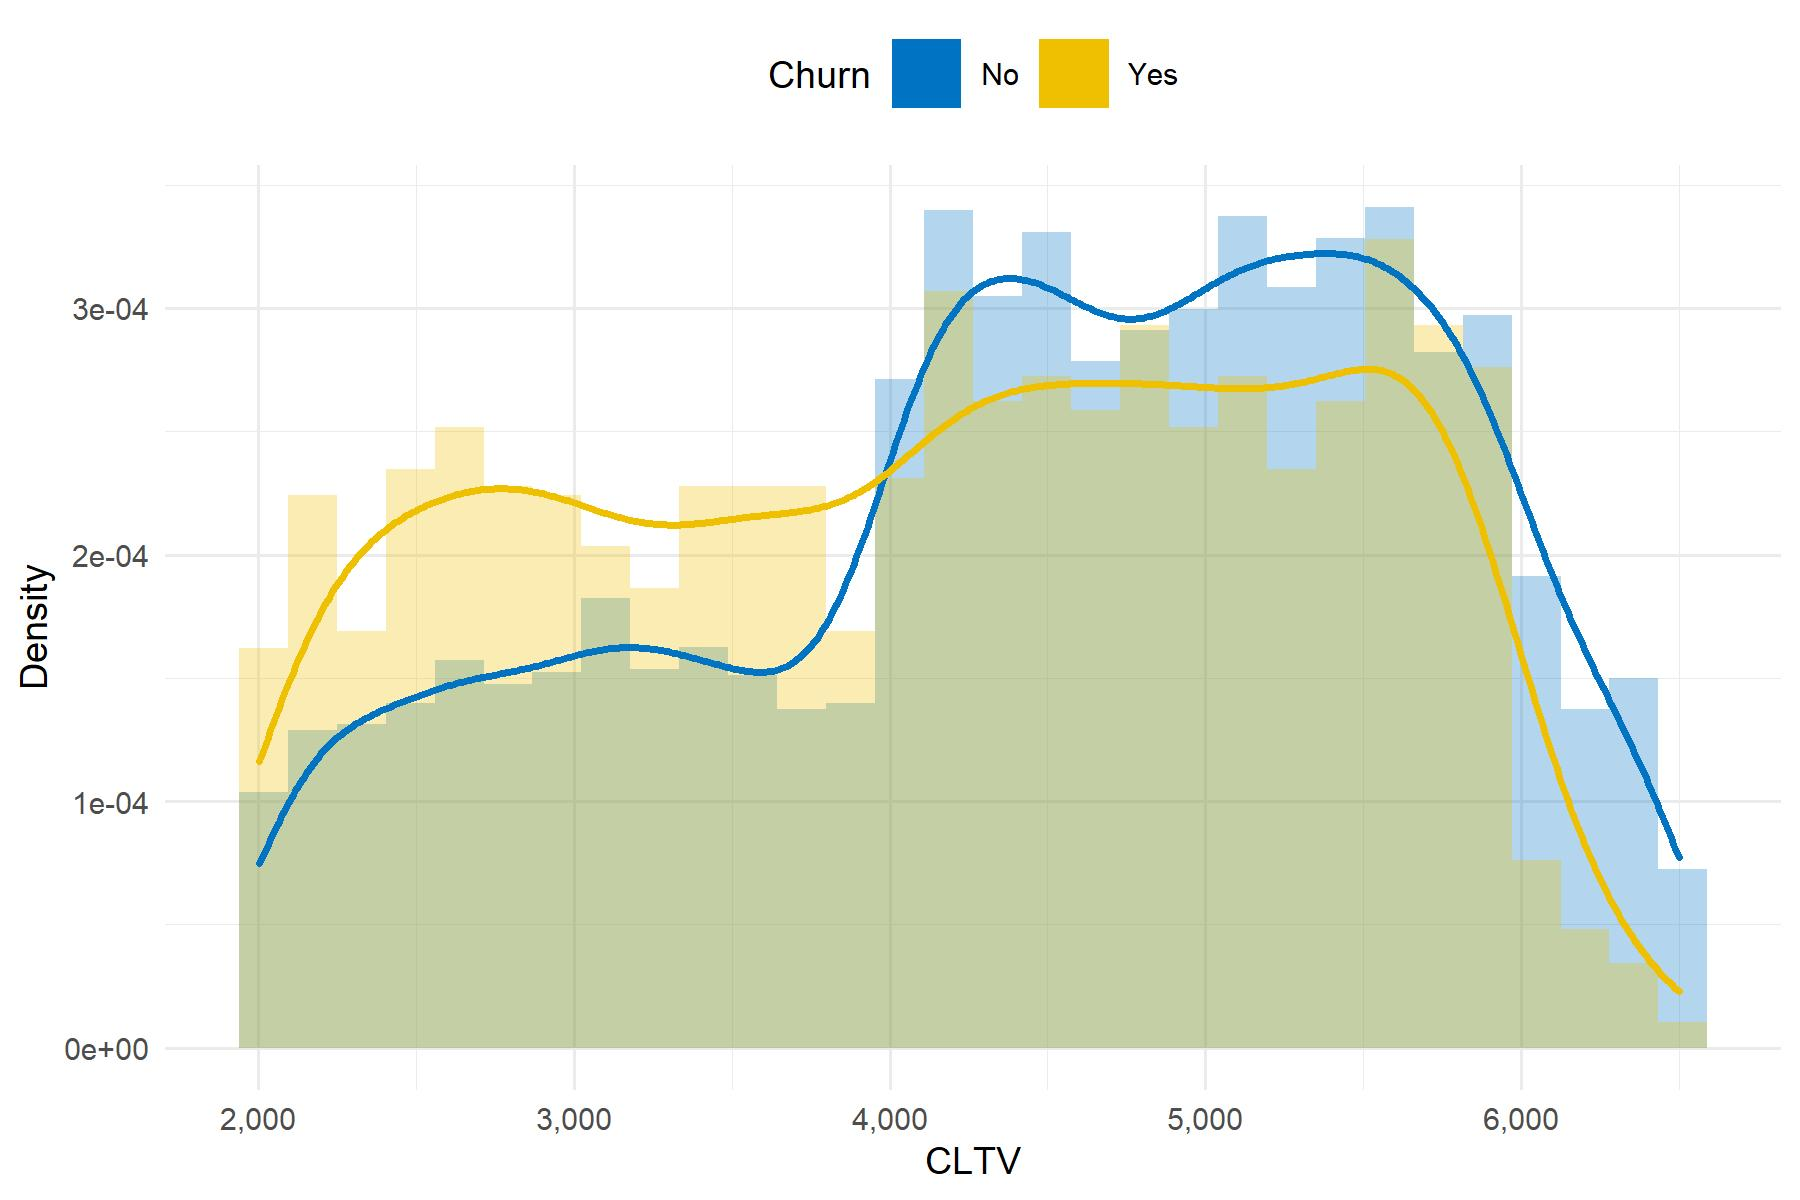
\includegraphics[width=450pt,height=350pt]{./imgs/cltv_churn_plot} 

}

\caption{Customer lifetime value depending on churn status}\label{fig:cltvchurn}
\end{figure}

The following histograms are interesting to the extent that the distribution of \texttt{Tenure\_Months} depends on the churn status. From figure \ref{fig:churndur}, one can note an inflation of low and high values for retained customers. The distribution appears to be more homogeneous for retained clients than for churners. These last's tenure months distribution is decreasing and looks like a Poisson distribution with an inflation of low values.

\begin{figure}

{\centering 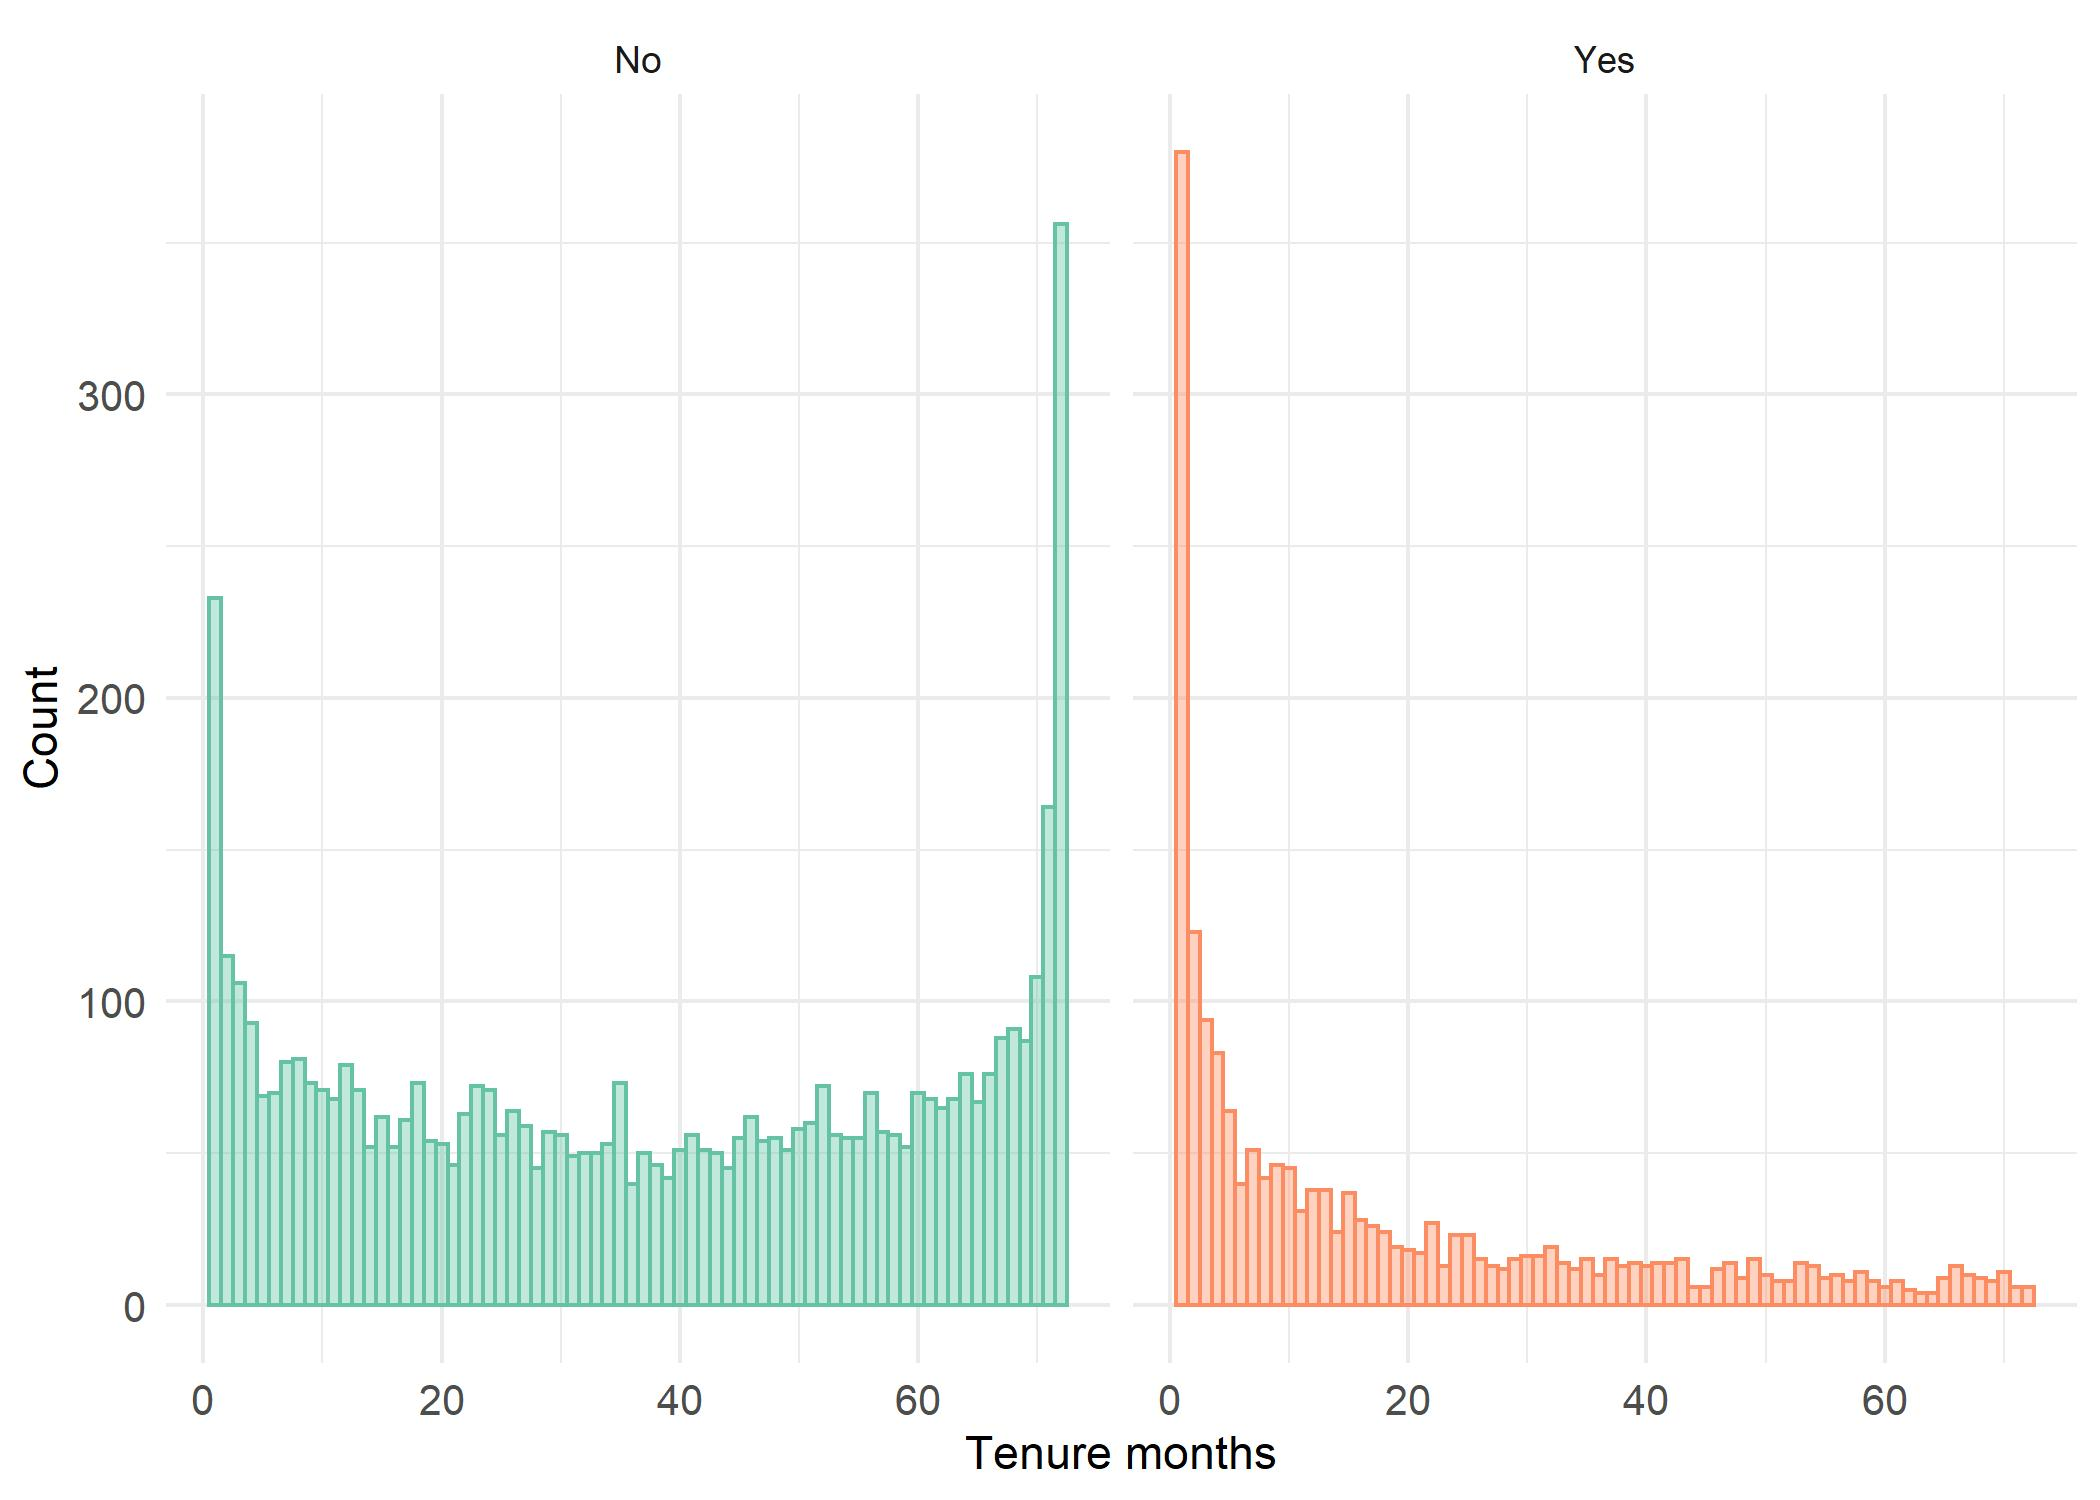
\includegraphics[width=500pt,height=350pt]{./imgs/duration_churn_plot} 

}

\caption{Tenure months depending on churn status}\label{fig:churndur}
\end{figure}

Eventually, the low \emph{p value} related to the Anova test between \texttt{CLTV} and \texttt{Churn\_Label} indicates that customer lifetime value is statistically different between churner and retained clients.

\begin{table}[H]

\caption{\label{tab:aovcltvchurn}Anova test between CLTV and churn status}
\centering
\begin{tabular}[t]{lrrrl}
\toprule
  & F statistic & Df1 & Df2 & p-value\\
\midrule
\cellcolor{gray!6}{Churn\_Label} & \cellcolor{gray!6}{117.57} & \cellcolor{gray!6}{1} & \cellcolor{gray!6}{7030} & \cellcolor{gray!6}{3.5e-27}\\
\bottomrule
\end{tabular}
\end{table}

\hypertarget{appendix}{%
\chapter*{Appendix}\label{appendix}}
\addcontentsline{toc}{chapter}{Appendix}

Some proofs of the mathematical concepts used in the study are derived, specifically related to duration analysis.

\hypertarget{hazard-function}{%
\section*{Hazard function}\label{hazard-function}}
\addcontentsline{toc}{section}{Hazard function}

\begin{equation}    
  \begin{aligned}
  \lambda(t) & = \lim_{\Delta t \to 0} \frac{P\big[t \leq T < t + \Delta t | T \geq t \big]}{\Delta t} \\\\
  & = \lim_{\Delta t \to 0} \frac{P\big[t \leq T < t + \Delta t \big] / P\big[T \geq t  \big]}{\Delta t} \\\\
  & = \lim_{\Delta t \to 0} \frac{\big(F(t+\Delta t)-F(t)\big) / \Delta t}{S(t)} \\\\
  & = \frac{\text{d} F(t) / \text{d} t}{S(t)} \\\\
  & = \frac{f(t)}{S(t)} \\\\
  & = - \frac{\text{d}S(t) / \text{d} t}{S(t)} \\\\
  \lambda(t) & = \frac{-\text{d} \ln \big(S(t)\big)}{\text{d} t}
  \end{aligned}
  \label{eq:hazfunproof}
\end{equation}

\hypertarget{link-between-cumulative-hazard-and-survivor-functions}{%
\section*{Link between cumulative hazard and survivor functions}\label{link-between-cumulative-hazard-and-survivor-functions}}
\addcontentsline{toc}{section}{Link between cumulative hazard and survivor functions}

\begin{equation}
  \begin{aligned}
       & \Lambda(t) = \int_{0}^{t} \lambda(s)ds \\\\
  \iff & \Lambda(t) = \int_{0}^{t} \frac{f(s)}{S(s)}ds \\\\
  \iff & \Lambda(t) = -\ln \big(S(t)\big) \\\\
  \iff & S(t) = \exp \big(-\Lambda(t)\big)
  \end{aligned}
  \label{eq:linksurvcumhaz}
\end{equation}

\hypertarget{contribution-to-the-partial-likelihood-function-in-ph-models}{%
\section*{Contribution to the partial likelihood function in PH models}\label{contribution-to-the-partial-likelihood-function-in-ph-models}}
\addcontentsline{toc}{section}{Contribution to the partial likelihood function in PH models}

\begin{equation}
\begin{aligned}
  \mathbb{P}\big[T_j = t_j | R(t_j) \big] & = \frac{\mathbb{P}\big[T_j = t_j | T_j \geq t_j \big]}{\sum_{l \in R(t_j)} \ \mathbb{P}\big[T_l = t_l | T_l \geq t_j \big]} \\\\
  & = \frac{\lambda_j(t_j|\mathrm{x_j}, \beta)}{\sum_{l \in R(t_j)} \ \lambda_l(t_l|\mathrm{x_l}, \beta)} \\\\
  & = \frac{\lambda_0 (t_j, \alpha)\phi(\mathrm{x_j}, \beta)}{\sum_{l \in R(t_j)} \ \lambda_0 (t_j, \alpha)\phi(\mathrm{x_l}, \beta)} \\\\
  \mathbb{P}\big[T_j = t_j | R(t_j) \big] & = \frac{\phi(\mathrm{x_j}, \beta)}{\sum_{l \in R(t_j)} \phi(\mathrm{x_l}, \beta)}
\end{aligned}
\label{eq:contribpartiallikproof}
\end{equation}

\hypertarget{partial-likelihood-function-in-ph-models}{%
\section*{Partial likelihood function in PH models}\label{partial-likelihood-function-in-ph-models}}
\addcontentsline{toc}{section}{Partial likelihood function in PH models}

Based on equation \eqref{eq:contribpartiallik}, one can derive the probability that all spells completed at \(t_j\) ends in the \(j^{\text{th}}\) failure time, such that:

\begin{equation}
\begin{aligned}
  \mathcal{L}_{p,\ t_j} & = \mathbb{P}\big[T_1 = t_j, \dots, T_{d_j} = t_j \ | \ R(t_j)\big] \\\\
  & = \Pi_{m \in D(t_j)} \ \mathbb{P}\big[T_m = t_j | R(t_j) \big] \\\\
  & = \Pi_{m \in D(t_j)} \ \frac{\phi(\mathrm{x_m}, \beta)}{\sum_{l \in R(t_j)} \phi(\mathrm{x_l}, \beta)} \\\\
  & = \Pi_{m \in D(t_j)} \ \phi(\mathrm{x_m}, \beta) \times \Pi_{m \in D(t_j)} \ \frac{1}{\sum_{l \in R(t_j)} \phi(\mathrm{x_l}, \beta)} \\\\
  \mathcal{L}_{p,\ t_j} & = \frac{\Pi_{m \in D(t_j)} \ \phi(\mathrm{x_m}, \beta)}{\Big[\sum_{l \in R(t_j)} \phi(\mathrm{x_l}, \beta)\Big]^{d_j}}
\end{aligned}
\label{eq:partlikproof}
\end{equation}

The joint probability over the \(k\) ordered discrete failure times then becomes:

\begin{equation}
\begin{aligned}
  \mathcal{L}_p & = \Pi_{j=1}^{k} \ \mathcal{L}_{p,\ t_j} \\\\
  \mathcal{L}_p & = \Pi_{j=1}^{k} \ \frac{\Pi_{m \in D(t_j)} \ \phi(\mathrm{x_m}, \beta)}{\Big[\sum_{l \in R(t_j)} \phi(\mathrm{x_l}, \beta)\Big]^{d_j}}
\end{aligned}
\label{eq:partlikproofbis}
\end{equation}

  \bibliography{biblio.bib,packages.bib}

\end{document}
